%%% Local Variables:
%%% mode: latex
%%% TeX-master: t
%%% End:

%\documentclass[doctor,secret]{ucasthesis}
\documentclass[master]{ucasthesis}
%\documentclass[doctor]{ucasthesis}
% \documentclass[%
%   master|doctor, % mandatory option
%   secret,
%   arialtoc,arialtitle]{ucasthesis}

% 所有其他可能用到的包都统一放到这里了,可以根据自己的实际添加或者删除。
\usepackage{ucastils}
\usepackage{xeCJK}
\usepackage{algorithm}  
\usepackage{algpseudocode}  
\usepackage{amsmath}  
\renewcommand{\algorithmicrequire}{\textbf{Input:}}  % Use Input in the format of Algorithm  
\renewcommand{\algorithmicensure}{\textbf{Output:}} % Use Output in the format of Algorithm 

\setCJKmainfont[BoldFont=STSong, ItalicFont=STKaiti]{STSong}

%打印时用
\hypersetup{colorlinks=false}

\begin{document}


% 定义所有的eps文件在 figures 子目录下
\graphicspath{{figures/}}

%% 封面部分
\frontmatter

%%% Local Variables:
%%% mode: latex
%%% TeX-master: t
%%% End:
%\secretcontent{绝密}

\ctitle{分布式流式主题模型的设计与实现}
% 根据自己的情况选,不用这样复杂
\makeatletter

\makeatother

\cdegree{工学硕士}
\cdepartment[计算所]{中国科学院计算技术研究所}
\cmajor{计算机软件与理论}
\cauthor{郭天佑}
\csupervisor{郭嘉丰\hspace{1em}研究员}
\csupervisorplace{中国科学院计算技术研究所}
% 如果没有副指导老师或者联合指导老师,把下面两行相应的删除即可。

% 日期自动生成,如果你要自己写就改这个cdate
%\cdate{\CJKdigits{\the\year}年\CJKnumber{\the\month}月}
\cdate{二〇一七年五月}

% 博士后部分
% \cfirstdiscipline{计算机科学与技术}
% \cseconddiscipline{系统结构}
% \postdoctordate{2009年7月——2011年7月}

\etitle{The Design and Implementation of\\ Distributed Stream Topic Model}
% 这块比较复杂,需要分情况讨论:
% 1. 学术型硕士
%    \edegree:必须为Master of Arts或Master of Science(注意大小写)
%              “哲学、文学、历史学、法学、教育学、艺术学门类,公共管理学科
%               填写Master of Arts,其它填写Master of Science”
%    \emajor:“获得一级学科授权的学科填写一级学科名称,其它填写二级学科名称”
% 2. 学术型博士
%    \edegree:Doctor of Philosophy(注意大小写)
%    \emajor:“获得一级学科授权的学科填写一级学科名称,其它填写二级学科名称”

\edegree{Master of Science}
\eauthor{Guo Tianyou}
\edepartment{Institute of Computing Technology\\Chinese Academy of Sciences}
\emajor{Computer Software and Theory}
\esupervisor{Guo Jiafeng}

% 这个日期也会自动生成,你要改么?
\edate{May, 2017}

% 定义中英文摘要和关键字
\begin{cabstract}
主题模型作为一种能够挖掘文本语义的技术受到了研究者的青睐,并且在业界得到了广泛的应用。
在社交网络等领域中,主题模型是文本分类,检索以及推荐等应用的一项重要技术。

随着移动互联网的发展应用,社交网络等许多场景中数据的产生正呈现出越来越快的增长趋势。
许多数据都具有高速、海量、实时、突发等主要特性。
人们通常形象地将这类数据称为流式数据。

面对这种新型的数据流式特性,以往的主题模型的训练方法遭遇了巨大的挑战。
流式机器学习的主要挑战在于,根据流式数据的特性,算法必须满足使用内存大小固定,高效实时,并且能够克服数据变动带来的对模型训练的影响。
以往大部分的主题模型算法实现都采用了批量的学习方法,但是批量学习并不满足上述要求。

通过调研,本文发现流式主题模型的设计与实现的主要难题在于:
(1) 流式数据具有海量无限的体量,并且数据分布时刻发生变化; 
(2) 在社交网络等类似的数据环境下,不断会有新词出现,词表是动态增长的;海量参数的分布式存储与并行更新同步困难;
(3) 流式学习系统对算法实时性的要求极高;

本文主要工作是设计与实现高效的分布式流式主题模型,以应对上面提出的挑战。
首先,本文提出了一种针对流式数据的在线流式主题模型。
该模型能够有效地克服流式数据的无限性与变动性,
不仅算法能够动态地更新模型,而且具有概念迁移的能力。
然后,本文从算法实现的角度出发设计了稠密和稀疏并存的混合参数数据结构,解决了动态词表所带来的参数存储与更新的难题。
最后,本文提出了一种新的采样方法,大大降低了采样的复杂度,并在此基础上进一步优化了算法的实现,保证了系统对算法实时性的要求。
本文提出的分布式流式主题模型的实现是一种高效,实时的具有动态演化能力的主题模型。

\end{cabstract}

\ckeywords{流式学习, 主题模型, Metropolis-Hastings, 参数服务器}

\begin{eabstract}
Topic Model has been favored in mining text semantics, 
that is significantly concerned in researches and productions. 
In the domain of text mining applications, such as social network,
topic model is the key technology of text classification, retrieval and recommendation.

Nowadays, the generation of data on the Internet shows growing trend. 
Many of the data are unlimited, real-time, and rapid, especially in social network. 
These data are called stream data.

Train topic model with stream data is interesting and a tough task.
Stream learning is confronted with a few great challenges. According to the features of stream data, 
Stream learning system required algorithm to be fixed memory consumption, efficient and real-time, trained against volatile data distribution.
However, the traditional batch learning does not meet these requirements.
And the most efficient implementations of topic model usually trained by batch learning process with static data.

In this paper, we found the main troubles in the design and implementation of distributed stream topic model are:
(1) the stream data is unlimited and volatile.
(2) new words would appear at any time in scenarios like social network.
(3) the requirements of efficiency and real-time is significant to stream learning system;

In order to solve the problems addressed above, we introduced how to design and implement distributed stream topic model in this paper.
First, we introduced a new stream topic model, online stream topic model.
The model solved the problem of infinity and volatility of stream data, and could capture the evaluation of topics upon stream data.
Second, we designed a dense-sparse mixture parameter data structure that greatly reduce the space consumption and running time of the application.
Finally, we applied an efficient sampling strategy that takes the advantage of metropolis-hastings and alias table, 
which is much effective than original sampling method.
Our model is high-performance, real-time and has the ability to evolve.

\end{eabstract}

\ekeywords{Stream Learning, Topic Model, Metropolis-Hastings, Parameter Server}

%% 设置 PDF 文档的作者、主题等属性
\makeatletter
\ucas@setup@pdfinfo
\makeatother
\makecover


% 目录
\tableofcontents
% 插图索引
\listoffigures
% 表格索引
\listoftables
% 算法索引
\listofalgorithms
%
\listofequations

%% 正文部分
\mainmatter

\chapter{引言}
\label{chapter:intro}

\section{研究背景}
当今,人们应该庆幸能够出生在20世纪末,赶上了一个新的计算机技术浪潮,并身处在这个环境中。
有赖于计算机互联网技术,计算机存储和计算技术的快速发展,计算机应用已经深入地影响并改变了人类的生活。

随着计算机技术的广泛应用所带来的互联网信息爆炸,以及大数据处理技术发展已经不再是什么新鲜的话题了。
然而它们给人类带来的机遇和挑战从来不会中断和消逝,因为现代计算机技术的发展的动力正是来源于这种源源不断的冲击。
直面这些问题与挑战,本文以互联网的兴起为大背景,大数据处理技术为基础,展开了对分布式流式主题模型的设计与实现的探索。

\subsection{流式数据}

美国图灵奖得主,诺贝尔经济学奖获得者赫伯特$\cdot$西蒙(Herbert A.Simon, $1916\sim2001$)曾说过:“在信息时代,最稀缺的资源不在是信息本身,而是对信息的处理能力。”

什么是大数据,迄今没有公认的定义。相较于传统的数据,人们将大数据的特征总结为5个V,即体量大(volume)、速度快(velocity)、模态多(variety)、难辨识(veracity)和价值大密度低(value)\cite{cxq2014Survey}。但大数据的主要难点并不在于体量大,真正难以应付的问题来自于其他几种特性。在这种环境下,人们往往遇到的是非结构化,海量实时的文本、视频、语音数据。这些数据常常意味着更大的技术挑战和更复杂的计算,以及更长的计算时间。而在商业应用中,数据处理的时间和质量往往意味着利益。

在许多应用场景中,数据是一个无穷的序列,并且数据的来源各异,格式复杂多样,数据可能带有一些时序,但是有无法保证数据是按照时间顺序排列处理。通常这类数据被称为流式数据。在不同场景下流式数据呈现出不同的特征,但是他们仍然具有鲜明的共性:

(1) 无限性。在流式场景下,数据以元组为单位,以连续的数据流的形式持续地到达计算系统。

(2) 无序性。虽然每个元组会按照某种时间顺序产生,但是,数据并不是严格按照时间次序到达。

(3) 突发性。数据的流速大小、元组特性数量和数据格式无法被提前预知。

(4) 易失性。在流式场景下,累加的数据量非常巨大。通常来说,数据通过简单的计算之后便会被丢弃,而不会别存储。

(5) 实时性。流式数据不仅是实时产生的,而且要求实时的返回计算结果。短时间内无法返回结果的数据,将会很大的影响系统的性能。

许多分布式计算系统都可以实时或接近实时地处理流式数据。常见的处理系统包括Storm, Spark Streaming和Samza。
Storm是一个实时的数据计算系统,使用过程中会先设计好一个用于实时计算的拓扑结构。Storm的数据流单位是元组,每个元组都是一个不可变的数组。
Spark Streaming是核心Spark API的一个扩展。它并不会像Storm那样一次一个地处理数据流。而是在处理之前按照时间间隔预先将其切分为一批次一批次的批处理作业。数据流被抽象为DStream数据结构,每个微处理批次得到一个RDD。
Samza处理数据流是,会分别按次处理每条收到的消息,但是Samza的刘单位既不是元组也不是DStream,而是一条条消息。

\subsection{流式数据场景}
比较典型的流式计算场景包括金融银行业应用、互联网应用和物联网应用\cite{sun2013bdsc}。
在互联网应用场景中,用户通常通过实时发布和分享产生各类数据,这其中最为典型的包括twitter,微博等社交软件的使用。
据统计,互联网上的数据有$75\%$来自于个人用户,主要有文本,图片、音频和视频等数据形式。


随着互联网的快速发展和壮大,网络已经融入到我们生活的方方面面,
用户可以方便的使用互联网进行检索、购物、娱乐、交流等活动。
根据CNNIC发布的《第39次中国互联网发展状况统计报告》显示,截至2016年12月,
我国网民规模达7.31亿,相当于欧洲人口总量,互联网普及率达到$53.2\%$\cite{website:cnnic-39}。

\begin{figure}[htb]\centering
  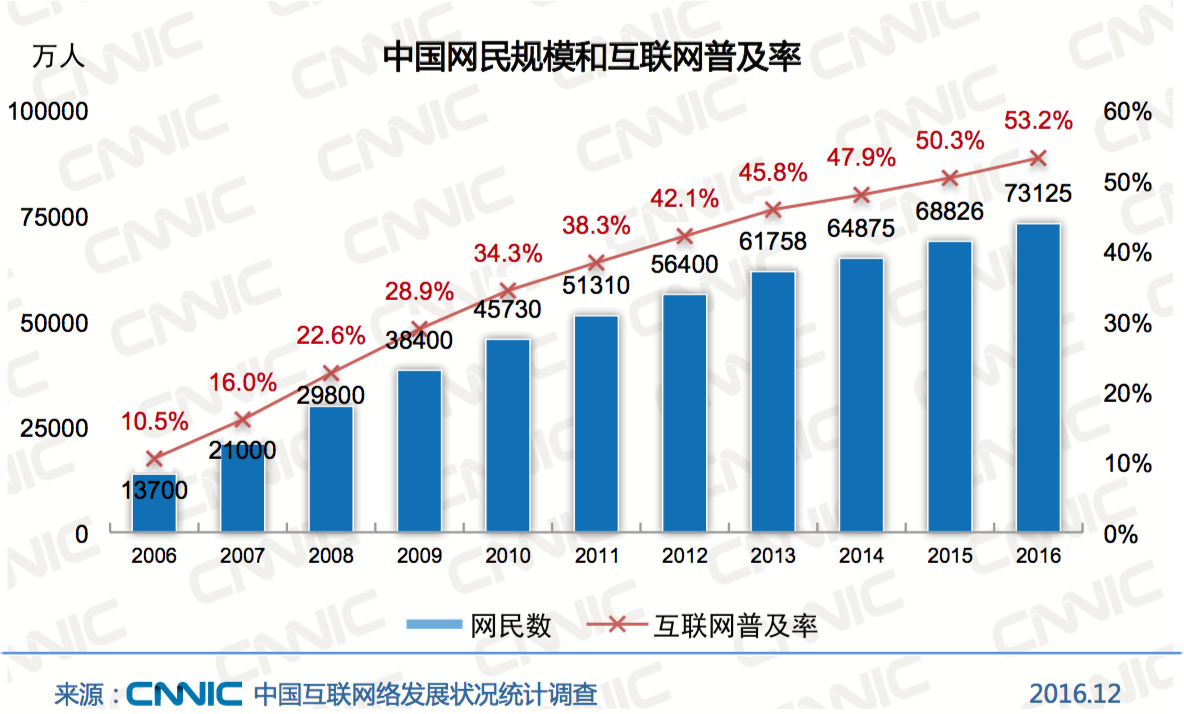
\includegraphics[width=0.7\linewidth]{cnnic-39-netuser}
\caption{中国网民规模和互联网普及率}
\label{fig:cnnic-39-netuser}       % Give a unique label
\end{figure}

社交网络以其快速灵活的方式己经逐渐改变人们交流的方式,用户可以在社交网络上进行沟通、分享、娱乐等活动。
以微博为例,微博是一个拥有庞大的用户基础,月活跃用户数(MAU)达到3亿的社交应用。
相对于传统的社交媒体,微博的时效性更强,影响范围更大,活跃度更高。微博月阅读量超百亿的领域达到了18个。
泛娱乐领域是微博活跃的主力场所;此外,在财经、教育、动漫等领域,微博同样发展迅速,颇受用户关注。
由于微博的流行与普及,微博信息数量呈爆炸式的增长,针对微博数据的处理和应用体现出典型的流式数据处理特征。

\subsection{流式数据与机器学习}
互联网的发展不仅推动了产业革命,同时也促进了机器学习人工智能的发展。人们常说在互联网时代,互联网是基础设施,数据就像原油。
那么机器学习就充当着高效提炼石油的技术。大数据与机器学习人工智能的结合,数据创造价值的关键。
每年Google,Facebook, Microsoft,百度,阿里等等国内外巨头公司都会在这些技术上有巨大的投入。
iResearch预测,2020年,中国人工智能市场将从2015年的12 亿人民币增长至 91 亿人民币。
2015 年,约 14 亿资本(年增长率 $76\%$)流入了中国的人工智能市场。机器学习人工智能俨然已经成为了各大公司的必争之地。

如上面所提及的,社交网络数据带有典型的流式数据特征,类似的场景还有许多。然而在流式数据环境下,传统的批量机器学习方法不再适用。
传统批量机器学习方法在流式数据环境下遇到了如下几个限制:

(1) 有限性

批量机器学习算法为了优化目标函数,会存储有限的训练集。流式数据具有无限性,数据持续的产生和输入,而无法完全存储在内存中。

(2) 迭代性

批量机器学习算法一般需要多轮迭代。在流式场景下,数据具有易失性和实时性,因此对算法的时间效率要求很高。通常数据仅经过简单的计算之后便会被丢弃。
因而,迭代性无法得到保障。

(3) 稳定性

批量机器学习算法都是基于独立同分布假设的。流式环境下,数据的分布可能随时间的推移而变动。因而,独立同分布假设无法得到保证。

(4) 静态性

批量机器学习算法训练得到的模型是静态的。在流式环境下,模型通常需要被实时地更新。使用静态的模型,则模型需要被频繁的替换,从而会造成应用系统的不稳定。

针对这些问题研究者也提出了一些在流式数据上的机器学习算法。
这些算法通常考虑了模型在时间上的延续性,消耗较少的内存,对数据变动具有感知能力。

P.Domingos和G.Hulten\cite{Domingos01catchingup}很好地总结了高效挖掘连续,高速,无尽的数据流学习系统的特性:

(1) 对每个数据样本只需要很少的运算时间

(2) 使用内存大小固定,与处理的样本数据总量无关

(3) 在构建模型的过程中,所有训练数据只会被计算一遍或少数几遍

(4) 随时产生独立于样本顺序的模型

(5) 具有概念迁移能力

\section{研究意义}
主题模型(Topic Model)在机器学习和文本挖掘领域是用来发现一系列文档中潜在语义主题的一种常用统计模型。
作为一个研究方向,主题模型受到了广大计算机科学家的爱戴,许多主题模型的方法被提出并应用于各个领域。
主题模型提供了一种从大规模数据中发现文本潜在语义只是的方法,并且将字词、文档映射到高维的语义空间上。
这种计算对很多语义相关的应用很有帮助,比如信息检索、推荐系统和社交网络等等。
许多公司都有自己的大规模主题模型实现,主要用于广告、推荐和检索等系统中。
不仅如此在生物信息,图像识别以及地理信息等其他学科领域主题模型也有相应的应用。

本文的主要工作是在流式数据环境下实现在线的主题模型。

当谈及流式机器学习的时候,人们往往需要:
(1) 模型具有时效性。比如天气,如果前两天的天气都是晴天40度,那么第三天下雪的可能性就几乎不可能了。
(2) 模型被经常更新。这需要模型对流数据的烟花和结构具有感知。

考虑到流式环境下模型的时效性要求高,模型更新频繁,批量机器学习算法不再适用。
现有的比较具有代表性的对规模主题模型实现包括LightLDA\cite{yuan2015lightlda}和PLDA+\cite{Liu:2011:PPL:1961189.1961198},以及Peacock\cite{Peacock}。
这些算法实现快速高效,扩展性也很好。但是,这些算法实现无一不是为静态数据集设计的。
而在流式数据环境下,算法将面临的是开放无限的数据集,持续增长的词表以及不断演变的数据分布。
显然,现有的算法无法克服上面的问题挑战。

解决这个流式数据上的机器学习的挑战常见的途径是增量学习和在线学习。
区别于批量学习,增量学习和在线学习每次只会适用一小批次的数据(而不是整个数据集),并且数据的信息也可能随着时间的变化而产生变化。
这类方法能够渐进地学习到知识更新演化,并且能修正和加强已有的知识,使得更新后的只是能够适应新的数据,而不必重新对全部数据进行迭代学习。
增量学习和在线学习降低了算法对时间和控件的要求,更适应与流式数据环境。

除此之外,在流式数据环境下主题模型的设计与实现仍然存在一系列挑战:

(1) 流式数据的特点带来的挑战

在流式数据环境下,数据带有实时性和无限性。而经典的主题模型实在静态数据上采用批量学习算法更新模型的,因而无法支持算法的实时性和在线更新。
除此之外,无限的数据意味着动态增长的词表,而词表的大小决定了主题模型的参数个数。根据词汇的幂律分布法则,我们知道随着时间的推移,不断会有新词出现,而绝大多数词汇确实低频词。

(2) 大规模的数据带来的挑战

在社交网络场景下,动辄上亿的数据使得单机机器学习算法无法快速实时地更新模型和作出即使响应。

(3) 主题模型拥有大规模的参数矩阵

主题模型的参数规模,数据词表大小以及主题的维度大小有关。主题模型的参数规模常常超出了一台服务所能存储的容量。不仅如此,在分布式环境下,更多的参数往往意味着更长的网络延迟。

面对如此复杂的算法和应用场景,对主题模型的研究不仅具有现实意义,而且还具有一定的代表性。比如,大规模流式数据上的机器学习模型和大规模参数模型,不仅仅在主题模型这个算法中会出现,同样还会出现在一些其他机器学习算法的应用中。

\section{本文贡献}
如上一节所述,传统的主题模型通常采用批量的机器学习方法训练。
不仅如此,分布式大规模的主题模型通常具有海量的模型参数。
这给模型训练带来了若干个棘手的问题,
a. 海量参数的分布式存储和并行同步;
b. 模型迭代时间随着主题模型规模的增长线性增长;
c. 无法适应持续增长的动态词表。

为了解决分布式流式数据环境下,主题模型实现遇到的挑战。
本文总结并分析了分布式流式数据环境下文本数据的特性,以及主题模型呈现出来的一些特征。
并在分析总结结果的基础之上,提出了分布式流式主题模型设计与实现的具体方案。
总体来说本文的主要贡献在于:

(1) 提出了分布式流式主题模型

大规模的分布式并行主题模型的实现得到了国内外各大公司的重视,在生产环境中得到了广泛的应用,产生了巨大的价值。
尽管这些算法实现具有高效稳定的特性,这些算法实现并不是针对流式数据设计的。
本文针对分布式流式数据提出了两个算法框架,分别是在线流式主题模型和增量流式主题模型。%,实验证明这两个算法是高效,稳定,收敛的。

(2) 采用了高效的Metropolis-Hastings算法

Gibbs采样算法是LDA主题模型参数估计一种主要方法。然而朴素的Gibbs采样算法是一种串行的坐标下降算法,不仅难以实现分布式并行,
而且采样算法的时间与主题维度大小线性相关。这种方法不适用于分布式大规模主题模型。
本文为了实现高效地执行主题模型算法训练过程中的MCMC采样,本文采用的采样算法使用了Alias Table和Metropolis-Hastings算法使得采样复杂度降低到了$O(1)$。
这种采样技术对于分布式流式主题模型的意义重大,不仅提高了采样的效率,同时令采样算法的时间复杂度不再与主题维度大小相关,模型得以训练更大规模的参数。

(3) 提出了稠密和稀疏并存的分布式参数数据结构

在LDA分布式Gibbs采样算法的实现中,参数词汇主题计数$n(w, t)$起到了关键作用。
如何选取和存储参数$n(w, t)$的数据结构,对算法效率的影响巨大。
因为对于超大规模的主题维度,$n(w,t)$中只有少数非零元,也就是说主题模型参数是一个非常稀疏的矩阵。
不仅如此,参数$n(w, t)$是一个与词汇相关的矩阵。在流式环境下,文本数据中不断有新词出现。
这意味着,分布式流式主题模型无法提前预知词汇表的大小,并且直接对主题模型参数进行存取会造成算法存储和时间效率大大降低。
本文提出的稠密和稀疏并存的分布式主题模型参数数据结构,有效地解决了上述两个问题,并大大提升了算法的执行效率。

(4) 优化了分布式流式主题模型的算法实现

本文在实现分布式流式主题模型时,采用了更加紧凑的4字节数据类型(int, float),而非8字节数据类型(long, double),节省了一般的存储空间并提升了网络传输的效率。
除此之外,本文算法还对算法采样顺序进行了优化,使得算法的参数降低了算法的同步代价。在此基础之上实现的参数Pipeline更新充分利用采样过程中的网络带宽。

\section{章节安排}
本文内容一共分为六章,每章内容组织如下:

第一章为引言部分,主要介绍了流式主题模型的相关背景意义和本文的主要贡献。
在本章中,本文首先介绍了流式数据的应用场景和特性,以及流式机器学习的主要难点。
接下来结合主题模型的应用,阐述了主题模型在流式数据上遇到的困难与挑战,
对于这些问题的研究不仅能够拓展主题模型在流式数据上的应用,而且对其他大规模流式机器学习具有参考意义。
最后介绍了本文的主要贡献。

第二章从两个方面介绍了国内外的相关工作以及研究现状。
第一个方面是关于流式学习的研究现状。流式数据挖掘的途径通常有两种一种是基于数据的方案,另外一种是基于任务的方案。
除此之外,本文还介绍了一些相对前沿的流式学习相关技术,主要是在线学习和增量学习技术。
另外一个方面是关于主题模型的研究现状。本文首先介绍了主题模型的发展历史和相关应用背景,之后又介绍了一些主题模型工作的变形。
最后介绍了大规模可扩展主题算法的实现和应用。

第三章介绍了流式主题模型算法设计。
本文首先总结和分析了常见的批量和在线主题模型方案。
本文指出流式主题模型不同于批量主题模型的设计,也不能套用简单的在线主题模型的设计,对于流式主题模型的设计需要考虑到流式数据主要特性。
本文结合了分布式和在线算法的设计思路,提出了两种大规模在线的流式主题模型。

第四章介绍了几种高效采样算法方案。在这一章,本文首先介绍了MCMC算法的应用及其基本理论背景,并介绍了基于MCMC方法的Metropolis-Hastings采样算法。
然后简要介绍了LDA的Gibbs采样算法。之后本文从主题模型的稀疏性出发详细分析和介绍了几种关于LDA的高效采样算法。
这些采样算法对分布式流式主题模型意义重大,它们不仅能够提升算法采样的效率,而且使得模型可以训练更大规模的参数。

第五章介绍了流式主题模型的实现。本章首先介绍了数据并行和模型并行对分布式并行算法的重要意义,以及参数服务器在分布式机器学习算法实现中的重要作用。
然后分析了流式数据环境下,词汇的主要特性和词汇对主题模型参数的影响。在此分析的结果之上,本章提出了稠密和稀疏并存的参数数据结构。
最后在本章提出的参数数据结构的基础之上,本文又介绍了几种优化实现分布式流式主题模型的具体方案。


\chapter{相关工作与国内外研究现状}
\label{chapter:relate}

\section{流式学习研究现状}

数据挖掘是一个跨学科的研究领域,用以从大数据中提取模型和模式\cite{hand1999statistics, hand2001principles, nialladamsadvances}
随着机器学习研究的进展,许多数据挖掘分析问题得到了解决。 
针对数据量持续增大的问题,研究者已经提出一些新的存储、机器学习和统计分析技术来处理可扩展性问题。

随着网络和并行计算技术的发展,新的分布式和并行机器学习数据挖掘算法也得到了发展。 
这些算法的目标是从数据集的不同子集中提取知识,并集成这些生成的知识结构,以获得整个数据集的全局模型。
为了缓解通信开销问题,一些客户/服务器,移动代理和混合模型算法也相应地被提出\cite{park2002distributed}。

近年来互联网技术的发展和应用,使得一些数据源中的数据生成速率比以往更快。
这种快速生成的连续数据息流对计算系统中的存储,计算和通信能力提出了挑战。

海量流式数据所带来的问题,通常可以通过两种途径解决,基于数据和基于任务的解决方案。 
在基于数据的解决方案中,算法仅检查整个数据集的一个子集,或将数据垂直或水平变换为近似较小的数据表示。
另一方面,在基于任务的解决方案中,通常采用计算理论的技术来实现时空效率的解决方案。

\subsection{基于数据的方案}
基于数据的方案通常指通过对整个流入的数据集者选取子集或者进行总结的方式来进行分析。
Sampling(采样), shedding和sketching是三种常见的选取子集的方式。摘要和汇总属于进行总结的方式。

\subsubsection{Sampling}
采样(Sampling)是指按照某中概率分布确定某一样本是否被选取的过程。
采样还可以细分为:领域采样,全局采样,水库采样以及不同采样。
在机器学习中如果使用采样策略,则计算误差的边界是采样率的函数,并使用Hoeffding边界来估计样本采样大小\cite{domingos2001general}。

采样算法的应用常见于如下问题:
\begin{itemize}
\item 在Cash Register数据流中查找不同项目的数量。见\cite{gibbons2001distinct}。
\item 在Cash Register数据流中查找分位数。有关最新的结果,请参见\cite{greenwald2001space}。
\item 在Cash Register数据流中查找频繁的项目。见\cite{manku2002approximate}。
\end{itemize}
 
这些问题都有很好的应用(除了上面引用之外还有很多其他的应用)。
此外,在高速流数据上实施采样也是相当实际的。 
(事实上,在一些监控数据流的系统中 - 特别是IP数据包嗅探器 - 
对流进行采样,只是为了将速率降低到合理的水平,但是一般都会按照某种既定的方式进行,否则有价值的信号可能会丢失。)
另外,保留样本有助于估计许多不同的统计信息。

在流式场景下,使用采样的问题是数据的大小无法提前预知。
因此,需要进行特殊的分析以找到误差边界。采样的另一个问题是,在一些问题场景中数据的异常对任务的影响很大,此时采样可能不是一种好的选择。
采样也不能解决数据速率波动的问题。

\subsubsection{Shedding}
Shedding指的是丢弃一些数据流序列的过程,在查询数据流应用中有比较广泛的应用\cite{babcock2003load, tatbul2003load}。
但是存在和Sampling类似的问题,并且难以应用到数据挖掘算法中。
因为,这种方法丢弃的数据会使得破坏数据的结构性,从而使得算法模型无法得到好的模式。

\subsubsection{Sketching}
Sketching主要依赖于降维,是对样本特征子集进行随机选取的过程,也就是数据流的垂直采样。
这种方法通常适用于Turnstile模型,因此非常普遍。

Indyk\cite{indyk2000stable}基于工作\cite{alon1996space}提出使用稳定分布来生成随机变量,具有不同稳定分布的Sketching相当于估计了数据流上的不同$L_p$范数。
比如使用高斯随机变量的Skeching可以很好地估计数据流的$L_2$范数,使用Cauchy分布可以得到$L_1$范数的良好估计。

Sketching还有许多变形,这些变形一般更为简单。 例如,随机子集\cite{gilbert2001surfing},Counting Sketches\cite{charikar2002finding}
以及Bloom filters\cite{broder2004network}。


从稳定的分布中采样产生一个随机变量序列的强大之处在于,这样一来,可以根据需要快速总结得到给定范围的属性。
而事实上这样的构造方法存在,并且可以快速生成样本并使用小空间。比如\cite{feigenbaum2002approximate}论文中提到的方法,\cite{gilbert2001surfing}中的Reed-Muller构造,
\cite{gilbert2002fast}中的$L_1$和$L_2$ Sketches的一般构造,以及\cite{cormode2003estimating}中$p\rightarrow0$的稳定分布的构造方法。

这种方法的主要缺点在于准确率,在一些场景中主成分分析会比这种方法更有效。

\subsection{基于任务的方案}
基于任务的技术是指那些为了解决流式计算挑战而修改或提出的新技术。近似算法,滑动窗口以及算法输出粒度属于这一类。

\subsubsection{近似算法}

近似算法\cite{muthukrishnan2005data}根源在于算法设计。它涉及计算难题的算法设计。 这些算法可以产生具有误差边界的近似解。
这种思路考虑到受到流式数据特性,在流式数据上的挖掘算法本身就是一个很难的问题。
近似算法作为解决流式数据机器学习和挖掘的解决方案,已经吸引了许多研究人员的兴趣\cite{cormode2005s}。
然而,近似算法并不能解决流式数据的速率的问题。

\subsubsection{滑动窗口}
使用滑动窗口技术的思想很自然,因为通常用户更关注最近数据。MAIDS\cite{dong2003online}系统使用了许多对于最近的数据的分析和总结技术。

\subsubsection{算法输出粒度}
算法的输出粒度(AOG)\cite{gaber2005board, gaber2004cost, gaber2004towards}引入了第一个资源感知的数据分析方法,可以根据存储器和时间约束来处理速率波动非常高的流式数据。
AOG在资源受限设备上执行本地数据分析。AOG有三个主要阶段。前两个阶段分别是适应资源和数据流速率,以及执行挖掘。
第三个阶段是在内存不足时合并生成的知识结构。 AOG已被用于聚类,分类和频率计算等任务中\cite{gaber2005board}。

\subsection{相关的技术}
流式数据被定义为具有超大规模,持续实时的数据。因而通常无法被完整地存储。
由于流式数据持续特性,数据的分布会受到概念迁移的影响\cite{minku2011online}。
执行在线数据流机器学习的主要要求是随着数据到达而同时做出更新学习的能力。
常见的机器学习算法如决策树是基于批量训练的,在进行训练之前需要大批量数据。
如果发生概念迁移,则需要重新训练模型\cite{zliobaite2011moa}。

在线学习是一种机器学习方法,在其学习过程中,数据一序列的顺序地输入,每条数据都会即使反馈并更新现有的模型。
与其相对应的批量学习则是每次没遍历完所有的训练集才会更新一次模型。
咋期限学习在机器学习领域中是一种常用的技术。在计算无法覆盖整个数据或者需要动态更新模型的情况下尤其适用。

在上世纪50年代,Rosenblatt\cite{rosenblatt1958perceptron}就已经提出了使用在线学习方法来实现感知器(perceptron)算法,可以解决线性可分问题。

流式学习和在线学习有着许多关联。可以说流式学习是在线学习的特例,数据都是按照一定步骤持续输入的,同时需要在线地更新模型。
除此之外,流式学习一般会受到资源的限制,而在线学习则没有明确的约束。

批量学习算法使用批量的训练数据来训练模型。然后使用训练出来的静态模型预测测试集上的样本。在线学习算法则初始化一个随机模型,
之后从训练群体中拾取一个观测样本,并重新校准每个输入参数的权重。

\begin{figure}[htb]\centering
  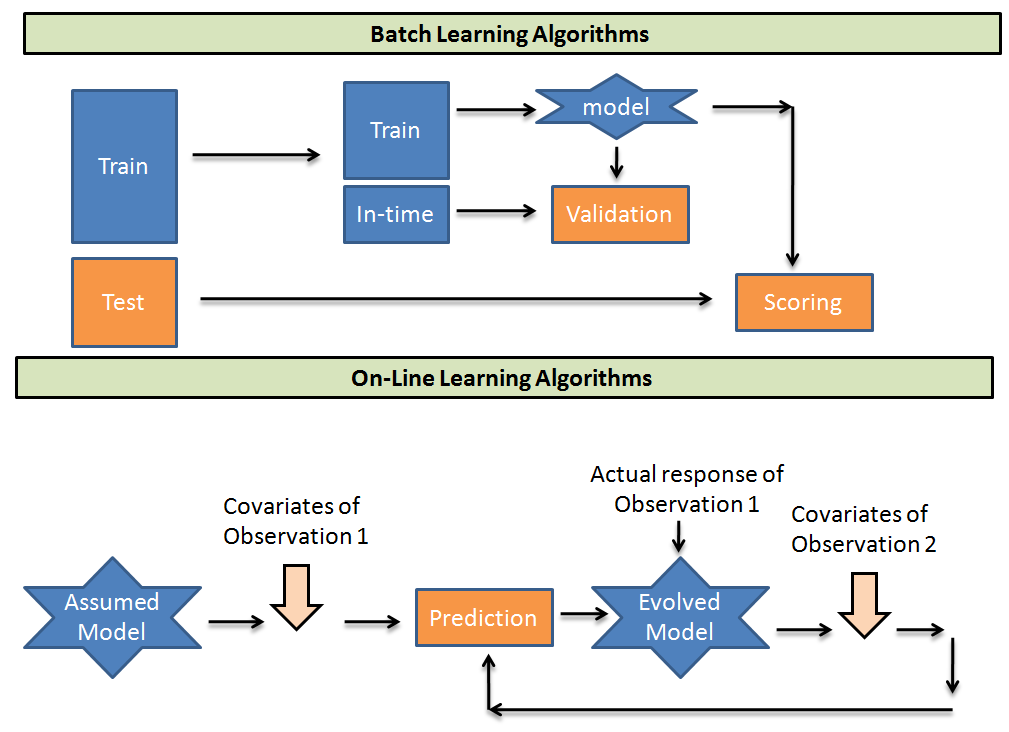
\includegraphics[width=0.7\linewidth]{batch-online}
  \caption{批量学习与在线学习方法对比}
  \label{fig:batch-online}       % Give a unique label
\end{figure}

增量式学习近来受到学术界和行业的日益关注。 从计算情报的角度来看,增量学习至关重要的至少有两个主要原因。
首先,从数据挖掘的角度来看,目前许多数据密集型计算应用需要学习算法能够从大型动态流数据中进行渐进式学习,
并随着时间的推移建立知识库,以使未来的学习和决策受益匪浅 处理。 第二,从机器智能的角度看,生物智能系统能够逐步学习信息。

\section{主题模型研究现状}
主题模型在机器学习和自然语言处理等领域是用来在一系列文档中发现潜在语义的一种统计模型。
其目标是高效第处理大型集合,并找到集合成员的表达,同时保留对基本任务(如分类,异常检测,总结以及相似性和相关性判断)有用的基本统计关系。

信息检索领域的研究人员最早在这类问题\cite{baeza1999modern}取得了重大进展。
IR研究人员为现代互联网搜索引擎成功部署的文本语料库提出的基本方法 - 将语料库中的每个文档表达为实数向量,每个元素都代表某个计量比。 
在流行的tf-idf方案\cite{salton1986introduction}中,研究者选择了基本词汇表,并且计算语料库中的每个文档,每个单词的出现次数。
在适当的归一化之后,将词频乘上逆文档频率(逆文档频率计数测量整个语料库中单词的出现次数)。
最终结果是得到一个词-文档矩阵$X$,其列包含语料库中每个文档的tf-idf向量。因此,tf-idf方案将任意长度的文档减少到固定长度的数字列表。

虽然tf-idf的规约具有一些吸引人的特征,该方法对维度的规约程度较小,并且难以表达文档内外部之间的交互信息。
为了解决这些缺点,IR研究人员还提出了几种其他降维技术,最著名的是潜在语义分析(LSA)\cite{deerwester1990indexing}。
LSA使用矩阵奇异值分解将tf-idf特征空间分解为多个线性子空间,同时保留了矩阵的大部分方差。
这种方法可以在大型集合中实现显著的压缩。 此外,Deerwester等人 认为LSA分解得到的特征是原始tf-idf特征的线性组合,捕捉到了一些基本语言概念,如同义词和多义词。

\begin{figure}[htb]\centering
  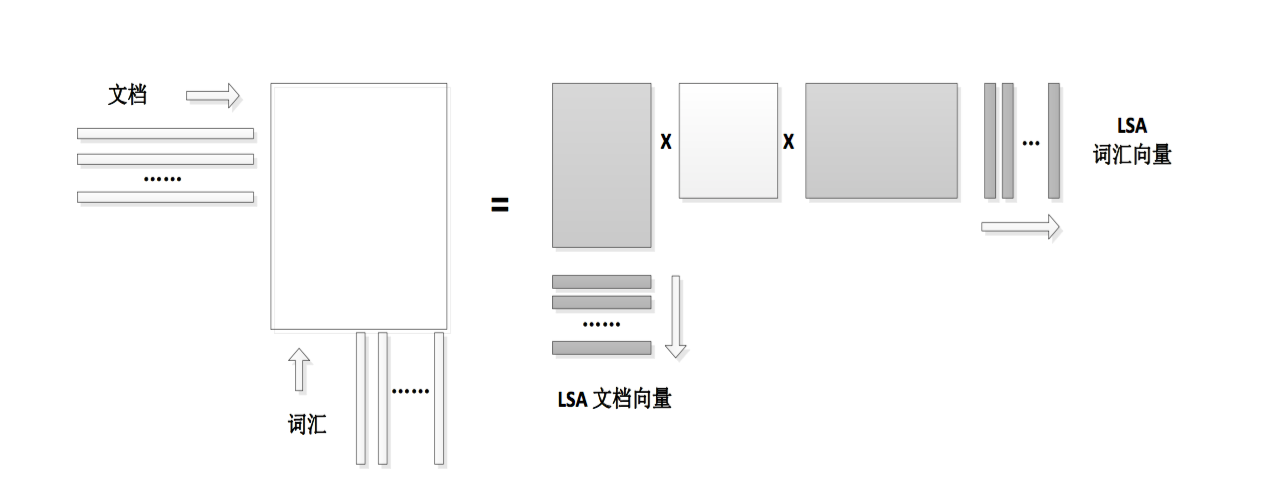
\includegraphics[width=1\linewidth]{LSA}
  \caption{LSA 对词文档矩阵的分解示意}
  \label{fig:LSA}% Give a unique label
\end{figure}

\subsection{主题模型简介}
1999年,Hofmann在论文\cite{hofmann1999probabilistic}中,提出了pLSA模型的重要工作,奠定了主题模型的基础。
PLSA 的出现和上世纪 90 年代兴起的潜在语义分析技术(LSA)有很大的关联,PLSA 可以看作是 LSA 模型在数理统计方面的扩展。
PLSA 简洁的模型让人更加 容易接触,并且使用概率统计知识对模型进行了论证使得模型有了更坚实的理论 基础,
并且 PLSA 模型的算法易于实现,可以适应分布式并行运算,适应了大数 据与分布式计算的时代潮流,最终使得 LSA 得到了强化和推广,大大地推动了 主题模型的研究浪潮。

PLSA方法将文档中的每个单词作为混合模型的样本进行建模,其中混合组件是可以被视为“主题”表示的多元随机变量。
因此,每个单词都是 从单个主题生成,并且可以从不同的主题生成文档中的不同单词。 
每个文档被表示为这些混合组分的混合比例的列表,从而映射到固定的主题集合上的概率分布。这种分布式表达可以用于表达文档特征。

\begin{figure}[htb]\centering
  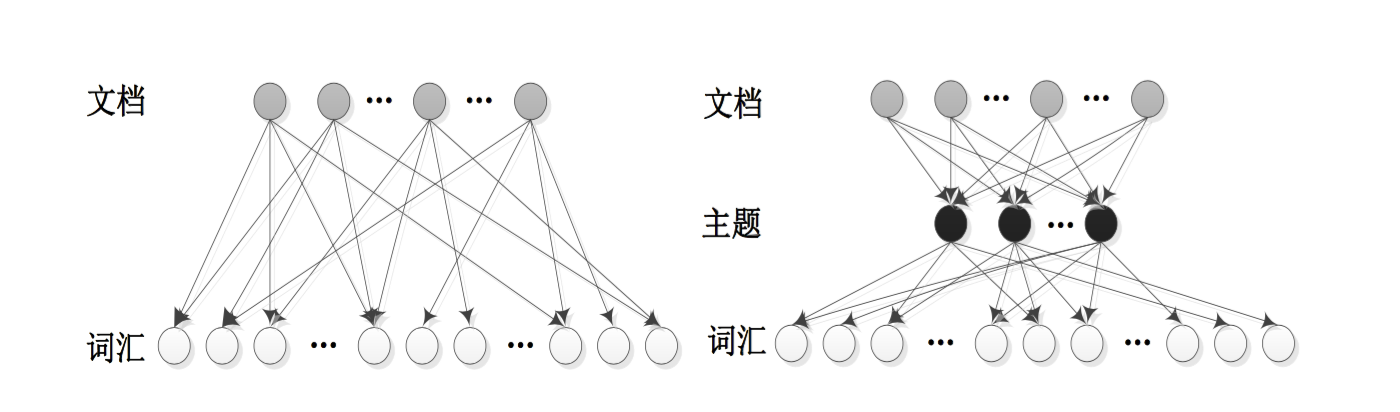
\includegraphics[width=0.9\linewidth]{topic-model}
  \caption{从词文档共现到引入潜在主题的概率模型}
  \label{fig:topic-model}% Give a unique label
\end{figure}

迄今虽然 只有十几年的历史,但是主题模型已经得到了很大的发展,在信息检索、文本分 类和信息抽取等自然语言处理领域得到了很广泛的应用,目前已经延伸至生物信 息学等其他领域。
在PLSA模型中,每个文档被表示成一系列主题概率分布,并且没有针对这些概率的生成模型。
这导致了以下两个主要问题:

(1) 模型的参数会随着训练数据的大小线性增长,不仅参数规模太大,还容易过拟合。

(2) 模型并没有明确给出如何给一个在训练集之外的文档分配概率。

LDA(Latent Dirichlet Allocation Model, LDA)\cite{blei2003latent}是主题模型领域的另外一篇经典之作,最初由David Blei, Andrew Ng, 和 Michael Jordan于2003年提出。
目前在各个领域得到了广泛的应用。不同PLSA的频率学派模型,LDA通过生成式模型克服了上面PLSA模型的主要问题。
该模型假设一篇文档主题分布是由Dirichlet先验分布生成的,同样一个主题下的词汇的分布也是由一个Dirichlet先验分布式生成的。

\begin{figure}[htb]\centering
  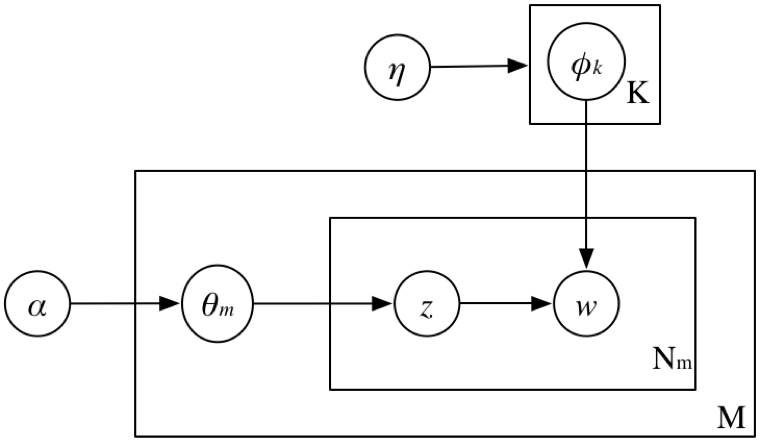
\includegraphics[width=0.7\linewidth]{LDA}
  \caption{LDA概率图模型示意}
  \label{fig:LDA}% Give a unique label
\end{figure}

\subsection{主题模型扩展变形}
在LDA模型提出之后,主题模型再次引起了广泛的关注。研究者又提出了许多LDA模型的变形和改进模型。

Blei等人提出的dDTM(Dynamic Topic Model, dDTM)\cite{blei2006dynamic}可以捕获在序列组织语料上的主题演变过程。
论文\cite{wang2012continuous}提出了cDTM(Continuous Dynamic Topic Model, cDTM)对dDTM进行了改进,使得模型的演变是连续的,而不是对时间进行了离散的分片。
论文\cite{wang2006topics}中也提出了时间上演变的主题模型,该模型显式地将时间建模到模型中去,并且没有做Markov假设。

主题模型通常基于"bag-of-words"假设,在这种假设中词汇之间相互独立,词顺序也相应地被忽略。
这对于那些n-gram模型来说是一个巨大的缺陷。
Wallach的工作\cite{wallach2006topic}提出了一个层次概率生成模型,该模型结合了2-gram的词组和unigram的主题模型,使得模型具有多元词组层次结构。

BTM(Biterm Topic Model, BTM) \cite{yan2013biterm}是主题模型的一种扩展,该模型考虑到了普通的主题模型比较适用于长文档,而对于短文本容易出现文档词共现稀疏的问题。
这种情况在Twitter和微博等场景中尤其常见。因而,模型参考了主题模型的思想在语料集合上构建二元词对集合,这种模型利用直接使用了词共现信息比LDA等模型得到词表达更能够反应词相关性。

在应用方面,主题模型同样有着非常多的变形。其中一些就是情感分析,用于分析文本语义的情感倾向性。
情感主题模型(Topic Setiment Model, TSM)\cite{mei2007topic}以及JSM(Joint Sentiment/Topic Model, JSM)\cite{lin2009joint}都提出了情感和主题混合的模型。
Titov和McDonald\cite{titov2008modeling, titov2008joint}采用了有监督信息并结合情感主题使得模型能够总结情感信息和文本。
除此之外,还有许多主题模型在情感分析领域的应用\cite{lu2011multi, jo2011aspect, li2010sentiment, si2013exploiting}。
在命名实体\cite{han2012entity, newman2006statistical, shu2009latent, kim2012etm}和学术作者识别\cite{rosen2004author}等工作中,主题模型一样得到了很好的应用。带有
带网络结构的主题模型(Topic Model with Network Sturcture, TMN)\cite{mei2008topic}是一种带有网络结构信息的文本主题模型。这种模型从用户角度考虑到互联网文本信息通常带有网络并对此建模。

不仅在文本类型的数据中,主题模型在其他类型的数据上也得到了应用,比如Fei-Fei Li等人将主题模型应用于图像分析\cite{fei2005bayesian, sivic2005discovering}, 
Pritchard\cite{pritchard2000inference}和Erosheva\cite{erosheva2002grade}将主题模型应用于人口调查。
据此,许多研究者都提出了类似的工作,加入上下文信息\cite{mei2006mixture}、时间\cite{wang2006topics}、地理位置和作者信息等等。

\subsection{大规模可扩展的算法应用}
上面的绝大多数数主题模型的工作都是在LDA模型的基础之上提出的。

最初LDA\cite{blei2003latent}提出的模型求解方法是变分推理(Variational Bayesian Inference, VB)\cite{jordan1999an},
这种方法引入了变分参数并利用Jensen不等式使得LDA模型变得更容易求解。
Griffiths\cite{griffiths2004finding}的CGBS(Collapsed Gibbs Sampling, CGBS)方法采用Gibbs采样的方法来求解模型参数。
Blei等人最初提出的VB方法相比,Griffiths的方法中采样空间是一个折叠的空间(通过积分消除了模型参数)使得模型的求解更适合于大数据的应用。
Teh\cite{teh2006a}等人参考了CGBS的工作提出了CVB方法(Collapsed Variational Bayesian Inference, CVB),这种方法不仅使得模型求解更加简便,
同时得到了比Blei等人的VB方法更好的误差下界,因而CVB方法拥有比VB方法更少的假设和约束。

FCGBS(Fast Collapsed Gibbs Sampling, FCGBS)\cite{porteous2008fast}针对CGBS优化方法采样效率较低(每次采样均的时间复杂度为O(K))的问题,提出了更快的算法。
类似的对采样进行加速的方法还有SparseLDA\cite{yao2009efficient}和AliasLDA\cite{li2014reducing}。

互联网海量规模的语料相对于精心设计的,清洗过的小数据来说要复杂得多。
在很多场景中,我们需要维持很大的词汇表和主题个数。因为小模型容易造成一些长尾低频词语义的丢失。
为了适应海量规模的数据和超大规模的参数,通常可以使用分布式并行策略来实现LDA模型(将数据分割存储在不同的机器结点上然后执行并行算法)。
这种方案可以在数千台机器数十亿篇文档上训练拥有上亿参数规模的模型\cite{Liu:2011:PPL:1961189.1961198, Peacock, ahmed2012scalable, li2014scaling, yuan2015lightlda}。 

YahooLDA\cite{ahmed2012scalable}和其它一些参数服务器分布式并行LDA实现\cite{li2014scaling},将词-主题共现计数作为全局共享的参数存储在参数服务器上。
而实际上这些参数会被存储在不同的机器上,从而使得参数规模可以达到更大。
另外,在分布式实现中数据被分成若干个子集存在不同机器结点上,每个子集上的词汇子集相比于全局的词汇表要小很多,因而在请求参数时模型只需要数据所需的部分参数即可。

LightLDA\cite{yuan2015lightlda}采用稀疏和稠密混合的参数服务器设计提高了内存和CPU效率,并且使用Word Proposal和Doc Proposal交替的方式使得采用时间效率达到了O(1)。

\section{本章小结}

本章主要介绍了流式学习和主题模型的相关工作与研究现状。

近年来,一些数据源的数据生成速率比以往更加快速,海量流式数据的机器学习和数据挖掘成为了许多研究者的研究热点。
针对流式数据的机器学习和数据挖掘主要分为基于数据的方案和基于任务的方案。
其中基于数据的方案主要包括采样,Shedding和Sketching等技术;基于任务的方案主要包括近似算法,滑动窗口和算法输出粒度等。
除此之外还介绍了在线学习和流式学习的关系和应用。

主题模型在信息检索和其它许多领域有着广泛的应用。针对不同的任务应用主题模型有许多响应的改进和扩展。
目前最为流行和应用最广的主题模型当属LDA模型。
在互联网海量数据的背景下,简单的LDA求解方式如CVB何CGBS方法效率和扩展性都太低。
研究者相应地提出了高效率,扩展性强的算法,如YahooLDA, PLDA+, Peacock以及LightLDA。这些工作实现了超大规模的LDA模型训练。

\chapter{流式主题模型算法设计}
\label{chapter:design}
大规模数据上的主题模型在国内外各大公司都得到了实现与应用,产生了重要的影响和价值。
流式数据环境下,主题模型的实现能够学习到主题的演化,并且动态地更新模型。
本章介绍了主题模型主要技术,并且提出了流式主题模型的设计。

\section{数学符号和术语}
本文通篇会使用到“词汇”,“文档”,“语料”,“主题”等术语。
比如,我们有时也会使用“隐变量”来表示用于标记抽象“主题”的变量。
为了避免这种歧义以及其他可能的问题,规范使用这些术语能够帮助描述和理解模型的设计。

如下,我们形式化地定义了一些术语与符号标记:
\begin{itemize}
\item 词汇:表示数据的基本单位,定义存在于一个词汇表中的元素。
\item 文档:表示为一个长度为$N$的词汇序列,$\mathbf{w}=(w_1, w_2, ..., w_N)$,其中$w_n$表示序列中的第$n$个词汇。
\item 语料:表示为一个大小为$M$的文档集合,$\mathbf{C=(w_1, w_2, ..., w_M)}$。
\item 主题:表示在文本预料集合$C$中语义内聚的多项式隐变量$z$。主题变量$z$的个数是一个有用户定义的常数$K$。
\item $\alpha, \eta$:表示Dirichlet模型的先验参数。
\item $\Theta, B$:表示LDA主题模型的后验参数。$\Theta=\mathbf{\{\theta_1, \theta_2, ...,\theta_M\}}$,
其中$\mathbf{\theta_m}$表示文档$\mathbf{w_m}$得到的主题分布。$B = \mathbf{ \{\beta_1, \beta_2, ...,\beta_K\}}$,
其中$\mathbf{\beta_k}$表示主题变量$z = k$的词汇分布。
\end{itemize}

\section{Latent Dirichlet Allocation(LDA)}
LDA的基本思路是将文档表示成主题随机变量的混合模型,每个主题表示为在词汇上的概率分布。
LDA提出的语料$C$文档生成过程描述如下:

0. 初始化参数$B$,$\{\beta_k \sim Dir(\eta_k)~ |~k \in [1, ... K]\}$

1. 从泊松分布中抽样第m篇文档的长度$N_m$,$N_m \sim Poisson(\xi)$

2. 从Dirichlet先验分布中抽样$\mathbf{\theta_m}$, $\mathbf{\theta_m} \sim Dir(\alpha_m)$

3. 抽样文档中的所有$N_m$个词项$w_n$:

~~~(a) 从多项式分布中抽样词项主题分配$z_n$,$z_n \sim Multinomial(\mathbf{\theta_m})$
   
~~~(b) 抽样一个词汇$w_n$,$w_n \sim p(w_n|\beta_{z_n})$

4. 对所有语料$C$中剩余的文档执行1 $\sim $ 3。\\
在上面的生成过程中,隐含着若干个假设:

(1) 给定主题模型的个数为$K$;

(2) 词生成概率矩阵$B$是一个$K \times V$的矩阵,$V$表示词汇表的大小;

(3) 每个文档的主题分布$\theta$都是$K$维的向量;

(4) 使用泊松分布作为文档长度的分布并不是决定的,如果有可以使用更好的分布;

(5) 文档长度$N$和其它主题模型的参数变量$\Theta, B, z$是相互独立的。\\
对于一个$K$维的Dirichlet变量$\mathbf{v}$落在一个$(K-1)$维的单纯形中(如果一个向量中的每个元素都不小于0,且总和为1,则落在$(K-1)$维的单存形中),
并且拥有如下概率密度:
\begin{equation}
Dir(\mathbf{v }| \mathbf{a} ) = \dfrac{\Gamma(\sum_{i=1}^K{a_i})}{\prod_{i=1}^K{\Gamma(a_i)}} 
v_1^{a_1-1} v_k^{a_k-1}
\end{equation}
其中,$\mathbf{a}$是一个$K$维的向量,且所有元素都大于0;$\Gamma(x)$表示Gamma函数。

Dirichlet函数对于单纯形来说是个简单的分布,它属于指数分布族,有有限的充分统计量。
Dirichlet还有一个重要的特性,这个特性便是和多项式分布式共轭。在许多应用中都会使用Dirichlet作为多项式分布的生成模型。

给定参数$\alpha, \eta$,参数$\Theta, B$,主题$\mathbf{z}$,数据$\mathbf{C}$的完全概率为:
\begin{equation}
p(\Theta, B, \mathbf{z, C} | \alpha, \eta) = \prod_{k=1}^K{Dir(\beta_k|\eta)}
\prod_{m=1}^M{\prod_{n=1}^N{Dir(\theta_m|\alpha)p(z_{mn}|\theta_m)p(w_{mn}|\beta_{z_{mn}})}}
\end{equation}
其中$p(z_{mn}|\theta_m)$表示主题取值为$z_mn$时的概率。通过积分,从上式可以得到数据集的概率:
\begin{equation}
p(\mathbf{C} | \alpha, \eta) = \prod_{k}^K{\prod_{m=1}^M{\int{Dir(\beta_k|\eta)} 
\int{Dir(\theta_m|\alpha)\prod_{n=1}^N{\sum_{z_{mn}}{p(z_{mn}|\theta_m)p(w_{mn}|\beta_{z_{mn}})}}}} d\theta_m }d\beta_k
\end{equation}

图\ref{fig:LDA}展示了LDA的概率图模型表示。图中$\theta_d$表示文档主题分布参数,$\beta_k$表示主题$z=k$的生成词概率分布。
$\alpha, \eta$分别表示LDA模型中文档主题分布$\theta_d$和主题生成词概率分布$\beta_k$的Dirichlet先验参数。
$z, w$表示每个文档中被采样生成的主题和词汇。

\begin{figure}[htb]\centering
  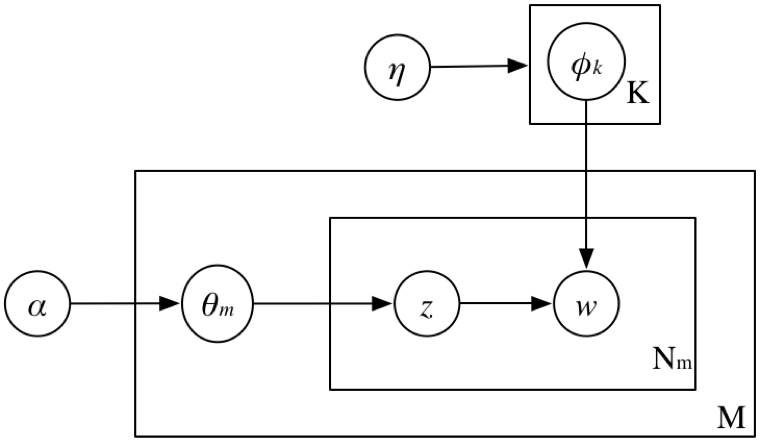
\includegraphics[width=0.5\linewidth]{LDA}
  \caption{LDA图模型表示}
  \label{fig:LDA}       % Give a unique label
\end{figure}

\subsection{批量LDA参数估计}
现有的LDA参数估计方法大多属于批量求解方法,主要包括两类算法,即变分方法和Gibbs采样。
前者的代表是Blei等人的VB方法\cite{blei2003latent}以及Teh等人的CVB\cite{teh2006a};
后者主要是Griffiths等人的CGBS\cite{griffiths2004finding}以及它的一些改进和扩展\cite{porteous2008fast, yao2009efficient, li2014reducing}。

在变分方法中,算法并非去直接估计真实的后验分布,而是借助另外一个更为简单的分布$q(z,\theta, \beta)$渐进地逼近正式的后验。
这些参数的最优值是通过最大化如下ELBO(Evidence Lower BOund, ELBO)得到的:
\begin{equation}
\log p(\mathbf{w} | \alpha, \eta) \ge L(\mathbf{w, \phi, \gamma, \lambda}) \triangleq 
\mathbb{E}_q{[\log p(\mathbf{w, z, \theta, \beta} | \alpha, \eta)]} - 
\mathbb{E}_q{[\log q(\mathbf{z, \theta, \beta})]}.
\end{equation}
其中$\phi, \gamma, \lambda$是变分方法引入变分参数,$\gamma$和$\lambda$分别是变分方法中$\theta$和$\beta$的Dirichlet先验。
值得强调的是,这里最大化ELBO等价于最小化分布$q(\mathbf{z, \theta, \beta})$和后验分布$p(\mathbf{z, \theta, \beta} | \mathbf{w}, \alpha, \eta)$之间的KL距离。

\begin{algorithm}[htb]  
\caption{ Batch Variational Bayes for LDA} 
\label{alg:bvb} 
\begin{algorithmic}[1] 
\Require Corpus $\mathbf{C = \{w_1, w_2, ..., w_M\}}$
\State Random initialize parameter $\lambda$
\While {relative improvement in $L(\mathbf{w, \phi, \gamma, \lambda}) > 0.00001$}
\State E step:
\For { m = 1 to M }
\State Set $\gamma_{mk} = 1$
\Repeat
\State Update $\phi_{mwk}, \gamma_{mk} $
\Until{ change in $\gamma_{mk} $ is relative small}
\EndFor
\State M step:
\State Update $\lambda_{kw}$
\EndWhile
\end{algorithmic}  
\end{algorithm}  

根据VB方法,可以得到上面的批量变分参数优化算法。

Gibbs采样算法是另一种主要LDA参数估计方法,并且更易于实现,因而在许多算法实现中得到了应用\cite{Liu:2011:PPL:1961189.1961198, Peacock, li2014scaling}。 

Gibbs采样算法(GiBbs Sampling)是马可夫蒙特卡洛(Markov-chain Monte Carlo, MCMC)算法的一种特例\cite{mackay2002information, hesterberg2012monte}。
MCMC算法的主要思路是构造一个非周期马氏链,并按照某一个转移概率反复地对马氏链的各个状态进行抽样,最终马氏链的状态分布会收敛于一个稳定的分布$\pi$。
虽然,我们无法直接获知$\pi$的具体值,但是我们仍然能够从分布中得到样本。
按照这种定义,只需要从分布中获取得到足够多的样本便可以很快地计算出稳定分布的近似估计$\hat{\pi}$。

\begin{figure}[htb]\centering
  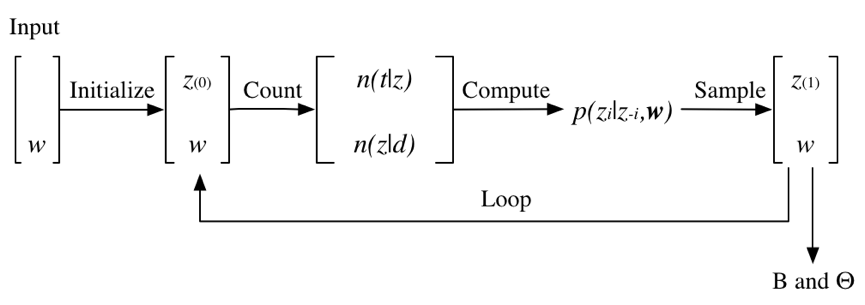
\includegraphics[width=0.8\linewidth]{Gibbs_Sampling}
  \caption{使用Gibbs采样算法学习LDA过程}
  \label{fig:Gibbs_Sampling}       % Give a unique label
\end{figure}

CGBS算法中提出的Gibbs采样算法通过积分消除了模型参数$\theta, \beta$,使得算法相比于直接的GBS算法能够更快地收敛:
\begin{equation}
\label{eq:pzw}
\begin{aligned}
p(\mathbf{z , w | \alpha, \eta}) &= p(\mathbf{w | z , \alpha, \eta}) p(\mathbf{z| \alpha, \eta}) \\
p(\mathbf{w | z, \alpha, \eta})                &= \left( \dfrac{\Gamma(V\eta)}{\Gamma(\eta)^V} \right)^K
\prod_{k=1}^K{\dfrac{ \prod_w^V \Gamma( n_{k,w} + \eta )}{\Gamma( n_{k, \cdot}+ V \eta)}} \\
p(\mathbf{z | \alpha, \eta})                    &=\left( \dfrac{\Gamma(K\alpha)}{\Gamma(\alpha)^K} \right)^M
\prod_{m=1}^M{\dfrac{ \prod_k^K \Gamma( n_{k,m} + \alpha)}{\Gamma( n_{\cdot, m}+ K \alpha)}} \\
\end{aligned}
\end{equation}
其中,$n_{k,w}$表示语料中词汇$w$的主题分配为$z=k$的计数,$n_{k, m}$表示文档中主题分配为$z=k$的词项的计数。
$n_{k, \cdot} = \sum_w^V{n_{k, w}} , n_{\bullet, m} = \sum_k^K{ n_{k, m}}$。

\begin{algorithm}[htb]
\caption{ Batch Collapsed Gibbs Sampling for LDA} 
\label{alg:bcgbs}
\begin{algorithmic}[1] 
\Require Corpus $\mathbf{C = \{w_1, w_2, ..., w_M\}}$
\State Random assign topic to each word in $\mathbf{C}$
\State Collect and summary $n_{k, w}$ and $n_{k, m}$
\While {Not converged or iter > MAX\_ITERATION}
\For { m = 1 to $M$ }
\For { n = 1 to $N_m$}
\State Sample $z_{mn} \sim p(z_{mn} | \mathbf{z}_{\neg (mn)}, \mathbf{w}) $
\State Update  $n_{k, w}$ and $n_{k, m}$ according to $z_{mn}$
\EndFor
\EndFor
\EndWhile
\end{algorithmic}  
\end{algorithm}  

借助式子\ref{eq:pzw},可以得到下面的抽样分布的定义:
\begin{equation}
\begin{aligned}
p( z_i = k | \mathbf{z}_{\neg i},  \mathbf{w}) 
&\propto p( z_i = k , w_i = t | \mathbf{z}_{\neg i}, \mathbf{w}_{\neg i}) \\
& = \dfrac{p(\mathbf{w |z}) p(\mathbf{z})}{p(\mathbf{w}_{\neg i} | \mathbf{z}_{\neg i})p(\mathbf{z}_{\neg i})} \\
& = \dfrac{ n_{k, w_i}^{\neg i,j} + \eta }{ n_{k, \cdot}^{\neg i,j} + V\eta}
\dfrac{n_{k, m}^{\neg i,j} + \alpha}{n_{\cdot, m}^{\neg i,j} + K \alpha}
\end{aligned} 
\end{equation}
其中$n^{\neg i,j}$表示不包括$z_i$的计数。这个抽样分布的式子很直观,
左边其实主题生成词概率的Dirichlet后验估计,右边则是文档主题分布的Dirichlet后验估计,正好反映了LDA模型先抽样主题,然后再抽样根据主题抽样词汇的生成过程。

算法\ref{alg:bcgbs}展示了批量CGBS的算法学习过程。
算法首先随机为语料中的每个词项分配一个主题,并统计$n_{k, w}$和$n_{k, m}$的值。
之后算法按照类似坐标轴下降的方法,顺序地抽样语料中的每个词汇的主题。
每个迭代将会遍历语料中所有的文档的所有词项。若干次迭代之后算法,最终会收敛。
值得注意的是,这边坐标轴下降方法中并不一定需要顺序地抽样语料中的每个词汇,实际上词汇之间先后的抽样顺序并不相关,可以按照任意顺序进行抽样。

批量的算法是LDA模型求解算法的主流算法,在语料大小可以完全被加载时,这种算法具有实现简单更加精确的优点。然而在数据量太大,数据分布不稳定的情况下,在线算法往往体现出来更好的性能。

\subsection{在线LDA参数估计}
\begin{algorithm}[htb]
\caption{Online Variational Bayes for LDA} 
\label{alg:olda}
\begin{algorithmic}[1] 
\State Define $\rho_t \triangleq (\tau_0 + t)^{-\kappa}$
\State Random initialize parameter $\lambda$
\For{ t = 0 to $\infty$}
\State E step:
\State Set $\gamma_{tk} = 1$
\Repeat
\State Update $\phi_{twk}, \gamma_{tk} $
\Until{ change in $\gamma_{tk} $ is relative small}
\State M step:
\State Update $\tilde{\lambda}_{kw}$
\State Set $\mathbf{\lambda}=(1- \rho_t) \mathbf{\lambda} + \rho_t \tilde{\mathbf{\lambda}}$
\EndFor
\end{algorithmic}  
\end{algorithm}  

在标准批量学习方法中,算法每一轮迭代都需要遍历整个数据集,这种计算方法带来的资源消耗非常高。
特别在主题模型应用中,这种现象更为常见——主题模型往往需要借助大规模的数据集上训练,
来挖掘人为无法标记的主题。虽然,使用分布式并行也能解决这种数据规模大的问题,但是这并不妨碍人们提出LDA参数估计的在线模型。

OLDA(Online Latent Dirichlet Allocation, OLDA)\cite{hoffman2010online}提出的在线VB方法将主题模型看作概率矩阵分解,并参考在线矩阵分解的技术\cite{mairal2010online},提出了如下在线算法\ref{alg:olda}。

算法\ref{alg:olda}中,语料集视为无穷大,并且按照时间分片一次一小批次地输入,所有词汇$w$来自于固定的词汇集$V$。
在整个算法执行过程中,$\lambda$起到了重要的作用,在这里$\lambda$参数表示LDA模型$\beta$的变分Dirichlet后验参数。随着时间的推移,$t$时刻之前的$\lambda$并没有被丢弃,而是通过一种衰减的方式保留下来。

衰减的权重设计为$\rho_t \triangleq (\tau_0 + t ) ^{-\kappa}$,这个式子中$\kappa \in (0.5, 1], \tau \ge 0$。
这么做的好处就是不断会有新的后验知识加入进来,并且旧的先验知识和后验知识的比例关系得到协调(时间越靠前的权重越小),使得模型在对全局的知识都有很好的掌握,,并很快地收敛。

On-Line LDA\cite{alsumait2008on-line}算法则从Gibbs采样算法的角度出发设计了在线LDA算法。

\begin{algorithm}[htb]
\caption{Online Gibbs Sampling for LDA} 
\label{alg:on-linelda}
\begin{algorithmic}[1]
\Require $ a, b, \omega^{\sigma}, S^t, t \in [1, +\infty)$
\For{ t = 1 to $\infty$}
\If{t == 1}
\State $\eta_k^t = b, k \in \{1, ..., K\}$
\Else
\State $\eta_k^t = B_k^{t-1} \omega^{\sigma}, k \in \{1, ..., K\}$
\EndIf
\State Random assign topic to each word in $S^t$
\For{ each word $w$ in $S^t$ }
\State GibbsSampling($S^t, \eta^{t - 1}, \alpha$)
\EndFor
\State Collect and summary $n_{k,w}^{(t)}$和$n_{k}^{(t)}$
\State Set $\beta_{k,w}^{(t)} = n_{k,w}^{(t)}$
\State Set $B_k^t = B_k^{t - 1} \cup \beta_k^{(t)}$
\EndFor
\end{algorithmic}  
\end{algorithm}  

算法\ref{alg:on-linelda}中,$\omega$是一个维度为$\sigma \time 1 $的向量,表示了时刻$t$之前的$\sigma$时刻内的$\beta$在先验中所占的权重。$\beta_k^t$是在$t$时刻词汇与主题$k$共现计数,是一个维度为$V^t \times 1$的向量。
$B_k^t$是一个$V^t \times \sigma$的演变矩阵。

通过这种窗口化的机制,算法不仅能够快速收敛,还能使得模型更聚焦于最近的数据。
对于那些时间太久远的潜在语义则有可能被遗忘,因而能够更精确地捕获主题在时间轴上的演变。
On-Line LDA借此将主题模型很好地应用于主题检测与跟踪。

\section{流式主题模型算法} 
流式数据带有显著的特性:无限性、无序性、突发性、易失性和实时性。
互联网社交网络和自媒体的广泛应用和发展,使得文本数据的增长速度越来越快。
并且网络上热议的话题经常因为各种现实世界的环境或者突发因素而改变(比如季节、社会事件等等),并且带有强烈的话题时效性。
\begin{figure}[htb]\centering
  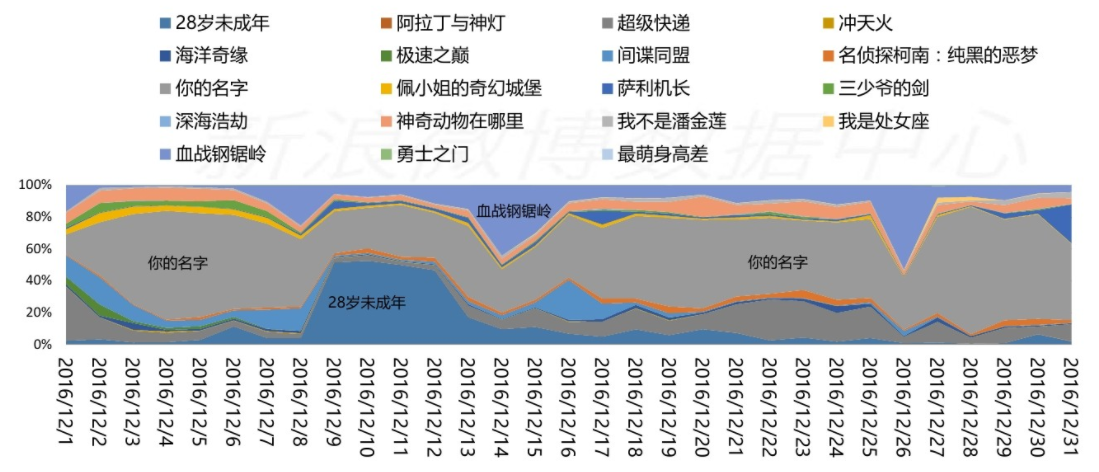
\includegraphics[width=1\linewidth]{movie-hot}
  \caption{2016年12月在映电影微博热议度变化趋势}
  \label{fig:LDA}       % Give a unique label
\end{figure}

对于此类数据,不仅内容演变快,同一时刻到达的数据量也非常可观。
大多数据公司都会采用分布式流式处理引擎来保证高吞吐率,高速率的数据处理。
常见的分布式流式计算引擎包括Storm,Spark Streaming和Samza。

可见海量的数据,频繁演变的主题趋势是一个很现实的问题。
如果仍然使用批量的算法来训练主题模型,那么在应用中不得不频繁地重新训练模型。
显然这种方法代价高昂,并且未必能够很好地利用所有的数据以及捕获主题的演变。
在线算法可以对主题演变进行良好的建模,但是目前的算法并没有提出大规模的分布式流式数据上的在线主题模型算法。

考虑到P.Domingos和G.Hulten\cite{Domingos01catchingup}提出
的数据流算法应该具有的特性:

(1) 对每个数据样本只需要很少的运算时间

(2) 使用内存大小固定,与处理的样本数据总量无关

(3) 在构建模型的过程中,所有训练数据只会被计算一遍或少数几遍

(4) 随时产生独立于样本顺序的模型

(5) 具有概念迁移能力。

在线流式主题模型的提出主要是受到了OLDA\cite{hoffman2010online}和On-Line LDA\cite{alsumait2008on-line}以及DTM\cite{blei2006dynamic, wang2012continuous}等论文的启发。

\begin{equation}
\label{eq:dir-gonge}
Dir(\mathbf{p} | \eta + \beta ) = Dir(\mathbf{p} | \eta ) + MultiCount( \beta )
\end{equation}

根据Dirichlet-Multinomial共轭\ref{eq:dir-gonge},$Dir(\mathbf{p} | \eta )$表示数据的先验分布,
$MultiCount(\beta)$表示观测到数据多项式统计,$Dir(\mathbf{p} | \eta)$表示给定先验分布与观测数据得到的相应后验分布。

\begin{figure}[htb]\centering
  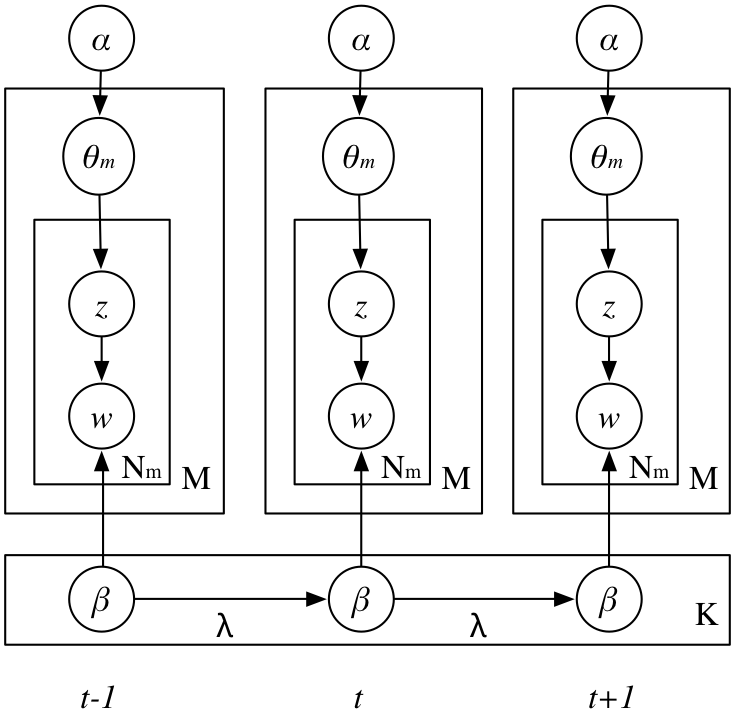
\includegraphics[width=0.5\linewidth]{graph-ostm}
  \caption{在线流式主题模型图模型表示}
  \label{fig:OSTM}       % Give a unique label
\end{figure}

如图\ref{fig:OSTM},该模型以流式计算为背景,将流式数据按照批次分割成不同的时间片。
仅有相邻的时间片模型之间产生关联。
图中$\beta$对应于$MultiCount(\beta)$多项式统计;图展示的是$t$时刻之后,算法将会得到一个后验的模型后验分布$Dir(\mathbf{p} | \eta + \beta_t)$。
为了使得$t$时刻训练得到的模型对$t+1$时刻的模型产生影响,本文的算法将$t$时刻的后验分布$Dir(\mathbf{p} | \eta + \beta_t )$作为
$t+1$时刻模型的先验分布。为了使得模型具有迁移演化能力,我们引入了$\lambda \in (0, 1)$表示衰减权重,应用于上一个时刻的观测数据之上。
最终在$t+1$时刻的模型先验分布可以表示为$Dir(\mathbf{p} | \eta + \lambda \beta_t )$。

本文的方法虽然与以往的一些工作有相似之处,但是存在明显的区别。
其中最重要的区别便是本文模型针对流式数据而提出,最终目标是方便实现大规模在线分布式并行采样算法的实现。
而DTM, OLDA以及On-Line LDA等模型并非针对流式数据的模型,因而无法适应在流式数据上的进行模型训练。

除此之外,DTM与OLDA均采用变分推理的方法来训练模型,而本文的方法使用了采样的方法,更有利于分布式并行实现。
DTM虽然对时间进行了建模,当时DTM是一个批量的学习算法,无法适应流式数据场景。
OLDA虽然采用了在线的学习算法,但是该算法并没有对模型的动态演变能力进行建模。

On-Line LDA与本文的模型一样都具有演变能力,同时也是基于采样算法实现。
但是On-Line LDA的模型先验分布表示为$Dir(\mathbf{p} | \eta + \sum_{i=1}^{win}{\beta_{t-i}} )$,
需要保存窗口$win$以内的所有历史数据,不仅对于拥有海量参数的大规模模型是无法容忍的,还会造成参数维护困难。
另外,本文提出的分布式MH采样算法效率要远远高于On-Line LDA采用的单机串行Gibbs采样算法。

\begin{algorithm}[]
\caption{Online Stream Topic Model}
\label{alg:onlineStreamLDA}
\textbf{\underline{Task Scheduler:}}
\begin{algorithmic}[1]
\Function{UPDATE\_VOCAB\&PARAMS}{$t$}
\State Collect and summary vocabulary $V^t$ at $S^t$
\State Add unkown words to $V_g$, $V_g = V_g \cup V^t$
\State Set $\beta^t(w, k) = \eta$, push $\beta^t(w, k)$, for $w \in (V_g - V^t)$, and update $\beta^t(k)$ accordingly.
\State Synchronize and pull parameter set $\beta^t(k), \beta^t(w, k)$ from servers
\State Set $\bigtriangleup \beta^t(k) = \lambda_t \beta^t(k), \bigtriangleup \beta^t(w, k) = \lambda_t \beta^t(w, k)$
\State Push $\bigtriangleup \beta^t(k), \bigtriangleup \beta^t(w, k)$  to servers and synchronize.
\EndFunction
\State Create a global vocabulary $V_g$
\For{ t = 1 to $\infty$}
\State Issue UPDATE\_VOCAB\&PARAMS(t)
\State Issue WORKER\_SAMPLE($t$) to all workers
\EndFor
\end{algorithmic}
\textbf{\underline{Workers $r = 1, ..., R$:}}
\begin{algorithmic}[1]
\Function{ LOAD\_DATA}{$t$}
\State Load a part of training data of $S^t$ as $C^t$
\State Pull the parameter set $\beta^t(k)$ and $\beta^t(w, k)$ from servers
\EndFunction
\Function{ WORKER\_SAMPLE}{$t$}
\State Issue LOAD\_DATA($t$)
\State Initialize topic assignment to each word in $C^t$ with prior knowledge.
\For{ each word $w$ in $C^t$ }
\State DO\_SAMPLING($C^t, \beta^t(k), \beta^t(w, k), \alpha$)
\EndFor
\State Collect and summary $n_{k,w}^{(t)}$ and $n_{k}^{(t)}$
\State Set $\bigtriangleup \beta^t(k) = n_{k}^{(t)}, \bigtriangleup \beta^t(w, k) = n_{k,w}^{(t)}$ and push $\bigtriangleup \beta^t(k), \bigtriangleup \beta^t(w, k)$ to servers
\EndFunction
\end{algorithmic}  
\textbf{\underline{Servers:}}
\begin{algorithmic}[1]
\Function{SERVER\_ITERATE}{$t$}
\State Aggregate $\bigtriangleup \beta^t(k) = \sum_r^R{\bigtriangleup \beta^t_r(k)}, \bigtriangleup \beta^t(w, k) = \sum_r^R{\bigtriangleup \beta^t_r(w, k)}$
\State $\beta^{(t+1)}(k) =\beta^t(k) +  \bigtriangleup \beta^t(k), \beta^{(t+1)}(w, k) = \beta^t(w, k) + \bigtriangleup \beta^t(w, k)$
\EndFunction
\end{algorithmic}
\end{algorithm}  

论文\cite{smola2010an}中提出了一种分布式并行Gibbs采样算法。在该分布式算法中,数据被均衡地分布式存储在不同的位置,
因而并行算法可以通过数据并行的方式实现。考虑到:
\begin{equation}
p( z_i = k | \mathbf{z}_{\neg i},  \mathbf{w}) 
 \propto \dfrac{ n_{k, w_i}^{\neg i,j} + \eta }{ n_{k, \cdot}^{\neg i,j} + V\eta}
(n_{k, m}^{\neg i,j} + \alpha)
\label{eq:sample-prob}
\end{equation}
主题抽样的概率只会依赖于$n_{k, w_i}^{\neg i,j}, n_{k, \cdot}^{\neg i,j}, n_{k, m}^{\neg i,j}$,因而与其他文档的主题计数无关。
主题模型并行采样算法的核心思想便是少数文档的采样并不会对全局主题分布$n(k)$和词汇-主题表$n(w, k)$造成很大的影响。
这意味着并行算法可以放松对$n(k)$和$n(w, k)$的同步(严格的同步极大的降低分布式算法的效率),从而可以加大算法的并行度同时保证算法收敛。
这种分布式模型并行思路被许多高效的主题模型分布式并行实现所采纳。

在本文的算法实现中我们延续了论文\cite{smola2010an}的思想,设置$n(k)$和$n(w, k)$为全局参数,
并假设在某些时刻这两个参数会得到同步(比如,以时间片为粒度)。

算法\ref{alg:onlineStreamLDA}总共分为三个部分Task Scheduler, Workers, Servers。
其中Task Scheduler是一个单机的算法调度模块,Workers是分布式并行的主要进程,Servers表示参数服务器。
$\lambda_t \in (0, 1)$表示衰减权重,可以有不同的定义。
这么做使得$\beta^t(k)$和$\beta^t(w, k)$拥有衰减的历史后验信息。
根据Dirichlet和多项式分布共轭的属性,我们将已观测到$\beta^t(w, k)$信息作为主题生成词多项式分布的Dirichlet先验。

流式主题模型算法迭代以时间为单位,在每个Worker的采样算法开始之前,各个Worker得到的模型参数是同步的。
而在每个时间片内部,所有的Worker之间是完全异步的,Worker进程之间的采样过程不需要互相等待。
另外在流式环境下,不断会有新词出现,模型必须能够动态的维护新词,本文将在后面的章节中讨论如何维护动态词表。

\section{实验分析}

\subsection{实验设置}
本文所有实验均采用如下设置,

\em{数据源:} 本文的实验数据均来自于某未公开动态实时数据,该数据中包含财经,体育,娱乐等多种类型内容;

\em{计算引擎:} 在本文的所有实验中,均采用了Spark Streaming作为流式计算引擎,拥有3台计算节点和1个参数服务器节点;

\em{节点信息:} Centos 6.6, 128G内存, 24 Intel(R) Xeon(R) CPU E5-2620 0 @ 2.00GHz。

\subsection{效果分析}
\begin{figure}[htb]\centering
  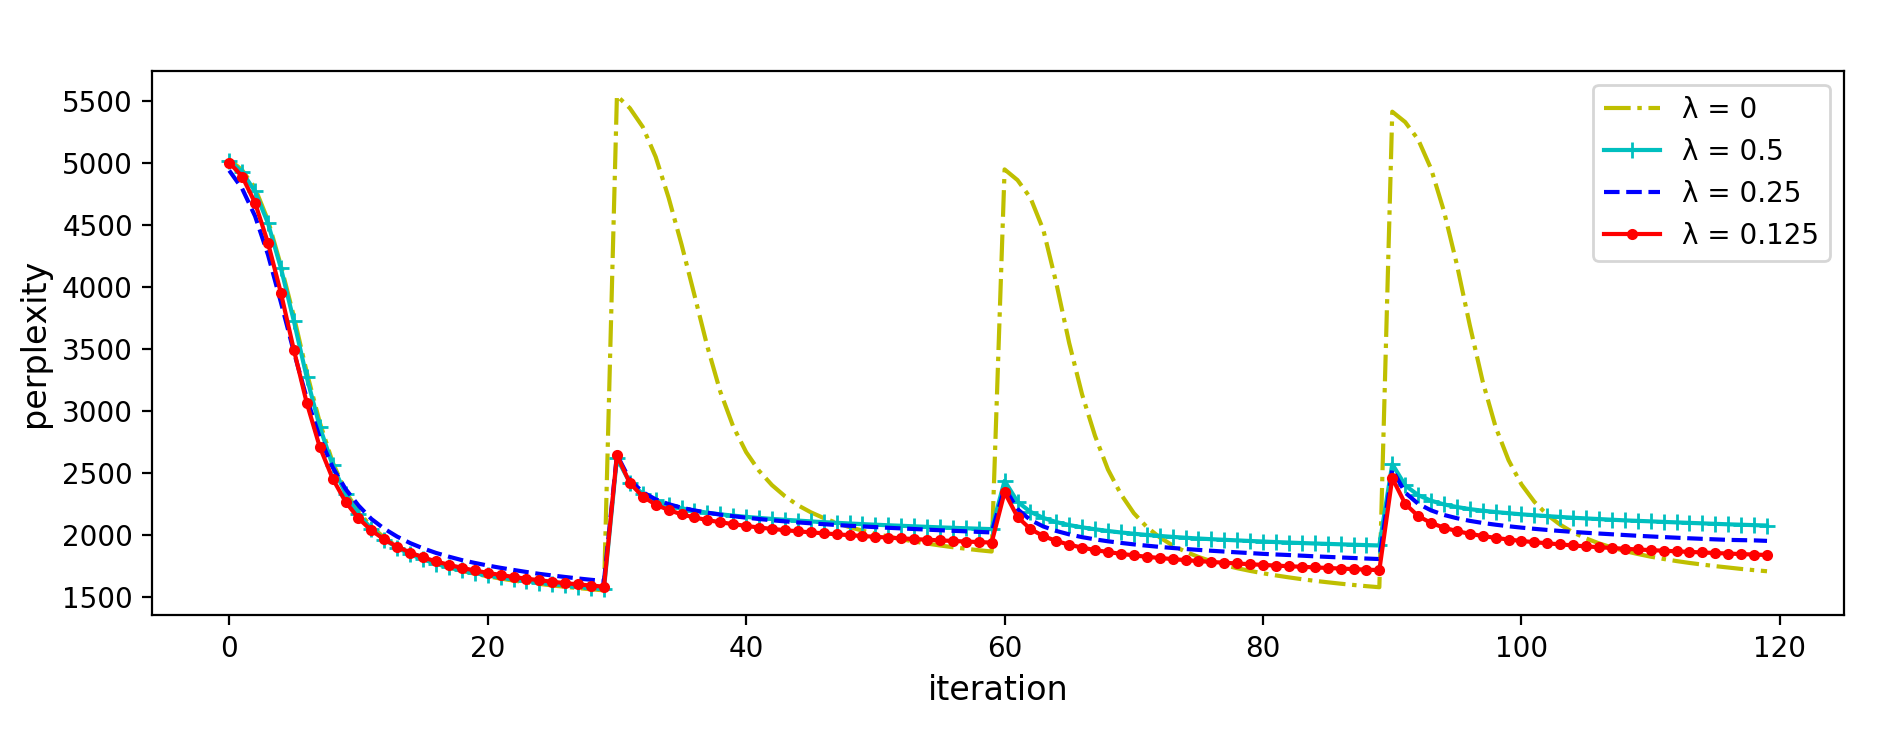
\includegraphics[width=1\linewidth]{exp-stream-perplexity}
  \caption{在线流式主题模型运行效果图}
  \label{fig:exp-stream-perplexity}       % Give a unique label
\end{figure}

上图\ref{fig:exp-stream-perplexity}展示的是在线流式主题模型在某一数据上的运行效果图。
图中评价指标为每个时间片数据上的Perplexity。
实验中我们设置了衰减权重主题模型个数$K = 100$,每个时间片10000个文档,每个时间片算法迭代30轮。
实验中我们共有4组实验,分别设置了$\lambda = 0, 0.5, 0.25, 0.125$。
不难发现,每个时间片上的主题模型训练都呈现出收敛的趋势,且衰减权重的设置对在线流式主题模型的效果影响重大。

当$\lambda = 0$时,也就是不考虑历史数据的影响,在线流式主题模型相当于重新训练主题模型;
当$\lambda \ne 0 $时,模型将历史数据作为先验,并且$\lambda$值越大模型受到先验的影响越大,收敛越快,但是Perplexity相对较大。
实际上,在许多机器学习的研究中都提到过先验知识能够提升模型的泛化能力。
先验知识太强也有可能使得模型在训练集上的效果变差。本文的实验正好符合这个现象。
在许多应用中,先验参数的选择是一个经验问题。特别在本文的在线应用场景中,我们很难确定什么参数最合适。
但这并不意味着我们无法选择一个合适的参数。比如,我们可以将在线实时的反馈结果作为选择参数的依据。

尽管我们并不知道最合适的参数是多少,但是我们发现本文的算法在不同的时间片上都具有收敛的态势。
只要参数设置合理,对于一批新数据模型能够迅速地收敛到一个比较好的位置,说明本文的算法具有适应新数据的能力。

\section{本章小结}
本章主要介绍了大规模流式主题模型的设计。首先介绍了LDA模型的基本理论背景,包括LDA模型的介绍,以及常见LDA参数估计方法。
从算法框架角度看,又有多种不同的批量估计方法和在估计方法。
在流式数据环境下,数据呈现出海量、高速、实时等特性。这些特性使得批量算法和简单的在线算法无法被直接应用。
因此,本文提出了一种大规模流式主题模型的设计方案。
该模型不同以往的主题模型,它是针对流式数据特性而设计的,便于高效的分布式采样算法的实现。
在后续的章节中,本文将更加详细地介绍如何高效地实现这种流式主题模型算法。

\chapter{流式主题模型的参数结构}
\label{chapter:parameter}
参数服务器的出现,使得分布式并行算法的实现更加简便高效。
目前已知的大规模高效主题模型算法的实现都采用了参数服务器\cite{li2014scaling}, 
比如YahooLDA\cite{ahmed2012scalable}, LightLDA\cite{yuan2015lightlda}, 以及Peacock\cite{li2014scaling}(只实现了模型并行服务,还未抽象出来参数服务器)。
本章将介绍使用参数服务器来构建的流式主题参数数据结构,以及在此基础上的一些具体算法优化方案和参数备份和恢复机制。

\section{参数服务器简介}
\subsection{数据并行}
数据并行指的是将数据进行分割,并分配给不同的计算节点并行地执行计算任务。
提及数据并行,我们往往能够想到Hadoop MapReduce和Spark等系统。

MapReduce通过简单的Mapper和Reducer的抽象提供的编程模型,可以在一个由几十到上百台的廉价机器集群上并发地,分布式地处理海量数据集,同时具有高可用性。
Spark则是一种内存的MapReduce扩展,Spark的核心数据结构是RDD(Resilient Distributed Dataset, RDD),该数据结构可以将数据持久化在内存中,从而避免了MapReduce不同阶段之间数据需要反复落盘的缺点。

这些系统允许一些严格同步的通信和迭代。借助这些大数据并行计算框架,有人开发了一些基于数据并行的机器学习库,比如Mahout\cite{mahout}, MLI\cite{sparks2013mli}。
这些算法库在小规模算法上效果尚可,一旦集群规模变大或者算法模型参数变多,算法执行过程中的需要大量的网络通信以及参数同步,网络的延迟和漫长的同步等待,会逐渐影响算法执行速度。

\subsection{模型并行}
模型并行指的是将大规模参数模型分布式地存储在不同机器节点上,并行地利用所有数据训练算法。
在算法训练过程中,每个分区会得到一部分参数子集的更新,在最终更新到模型之前通常会对各个分区的结果进行合并。
这种方法常用于具有大规模参数的模型同时数据分区不是很多的场景。
这种时候算法执行过程中不会频繁地进行网络通信,同时算法的每个分区只会使用和更新一小部分参数子集。
这种方法的优点是,算法同步的效率高,网络通信开销和延迟小。但是该方法通常需要每个工作分区完全加载所有的数据样本, 这在数据规模太大时是无法做到的。

\subsection{参数服务器}
上面提及的数据并行与模型并行方案都是单独使用的。
在现实业务场景中,机器学习算法的数据量和参数都可能非常之多,这使得单机无法完全加载训练数据或者无法加载存储所有参数。
此时结合数据并行与模型并行两种方案,是一种行之有效的方法。
但是同时应用这种两种方案往往使得程序的实现更加复杂,并且引入其他不稳定因素。

参数服务器很好地解决了数据并行和模型并行同时应用的难的问题。
参数服务器使得数据并行过程中,算法可以在不同分区访问和更新全局参数(模型并行)。
参数服务器的出现主要解决如下挑战:

(1) 访问参数会消耗大量的网络带宽。

(2) 许多机器学习算法在并行过程中的许多步骤需要同步,这种同步很可能造成巨大的延迟。

(3) 当机器学习算法规模大时,系统越来越容易出错。


\begin{figure}[htb]\centering
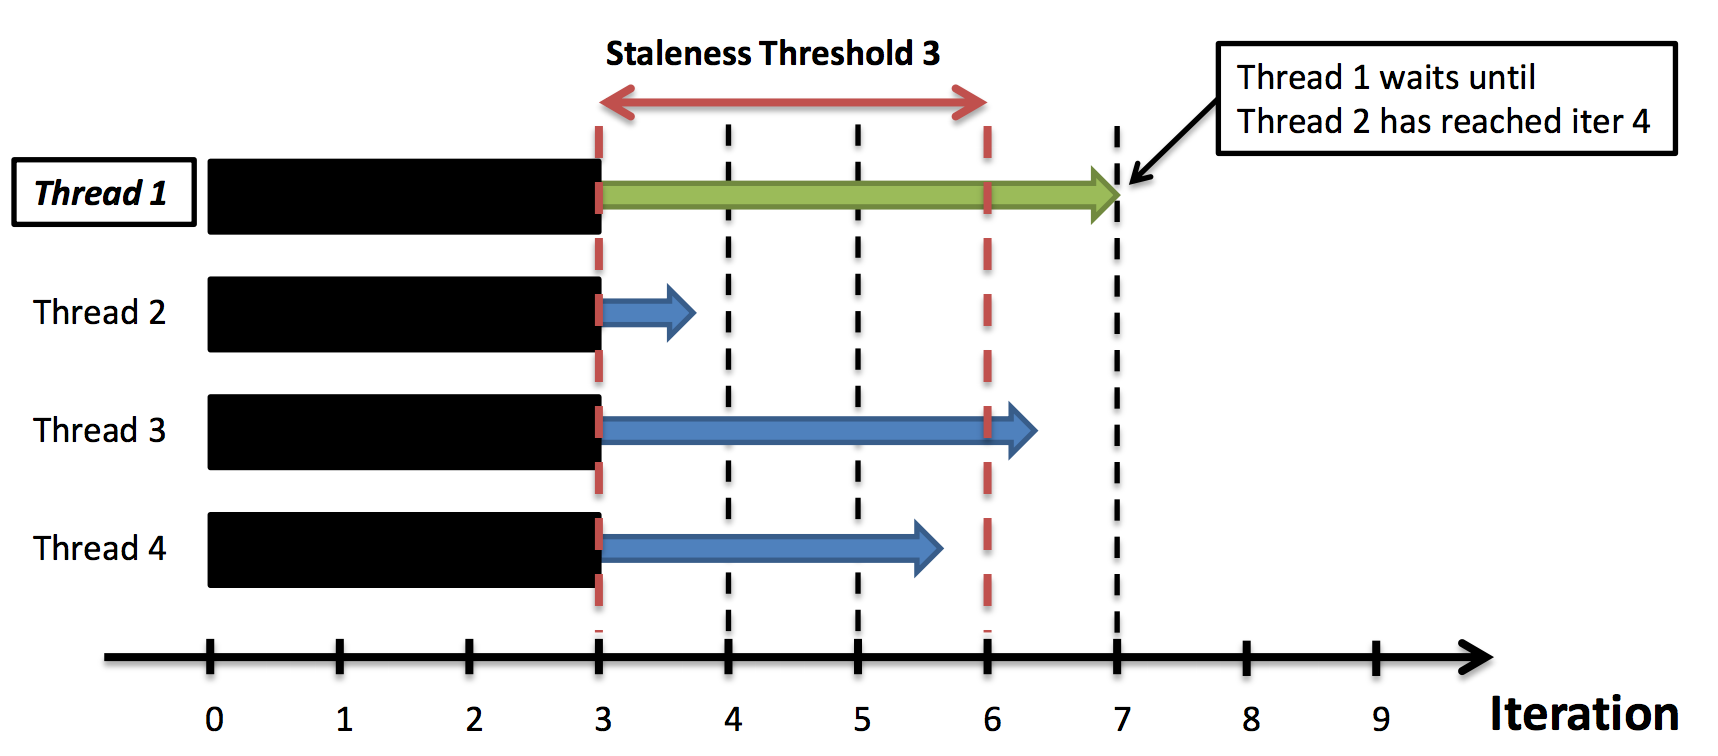
\includegraphics[width=0.8\linewidth]{SSP}
\caption{Stale Synchronous Parallel}
\label{fig:SSP}       % Give a unique label
\end{figure}

尽管如此,参数服务器作为一个通用性很强的中间,并不能解决所有的机器学习问题。
我们仍然可以从两个方向着手缓解上述的挑战,第一个方向是通过更好的参数服务器实现和设计来提供更高效的服务;
另外一个方向是从算法应用的角度出发,通过更好的算法设计和参数服务器使用,来减少网络通讯和延迟。
前者的主要方式有压缩传输,Pipeline, SSP(Stale Synchronous Parallel, SSP)等等。
后者的主要方式包括从应用的角度减少参数的访问,使用更小更紧凑的参数类型,更稀疏的参数表示等等。为此,接下来本章将主要介绍如何设计分布式流式主题模型的参数存储和使用。


\section{混合参数结构的设计}
在互联网环境下,流式数据没有尽头,人们无法提前预知数据的分布,因而数据流上不断会有未登录词出现。
我们知道词汇的分布服从幂率分布,也就说大语料中绝大多数出现的词汇属于低频词,并且在流式数据中呈现出线性增长的趋势,如图\ref{fig:power-law}, \ref{fig:noFreq2-5VsWords}。

\begin{figure}[htb]\centering
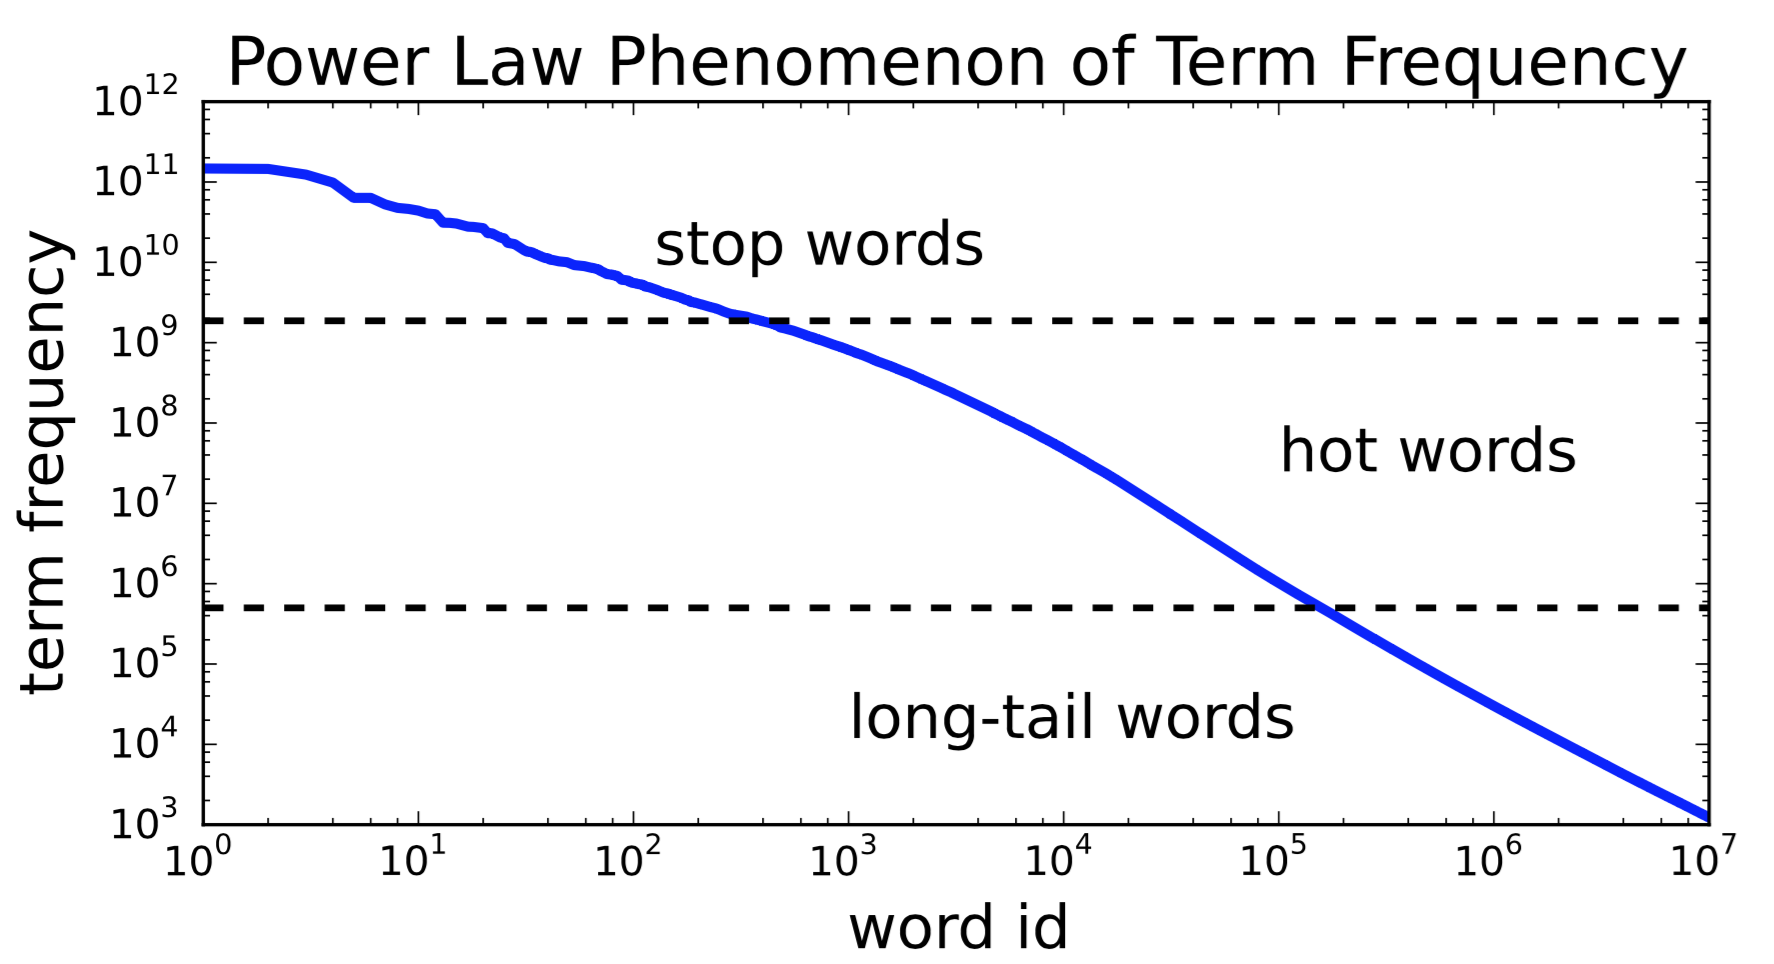
\includegraphics[width=0.5\linewidth]{power-law}
\caption{词频的幂率分布现象}
\label{fig:power-law}       % Give a unique label
\end{figure}

图\ref{fig:power-law}来自于论文\cite{yuan2015lightlda}, 是分析150亿个网页得到的结果,显示除了少量的静态词之外(几百上千),中间大约有几万-几十万个常用词,其他的词汇属于低频词。
论文\cite{yuan2015lightlda}还提到静态词和常用词大约只占所有词汇的$10\%$,而低频词却占了$90\%$。然而,静态词和常用词大约覆盖了$95\%$的语料,而低频词仅仅占了$5\%$。

\begin{figure}[htb]\centering
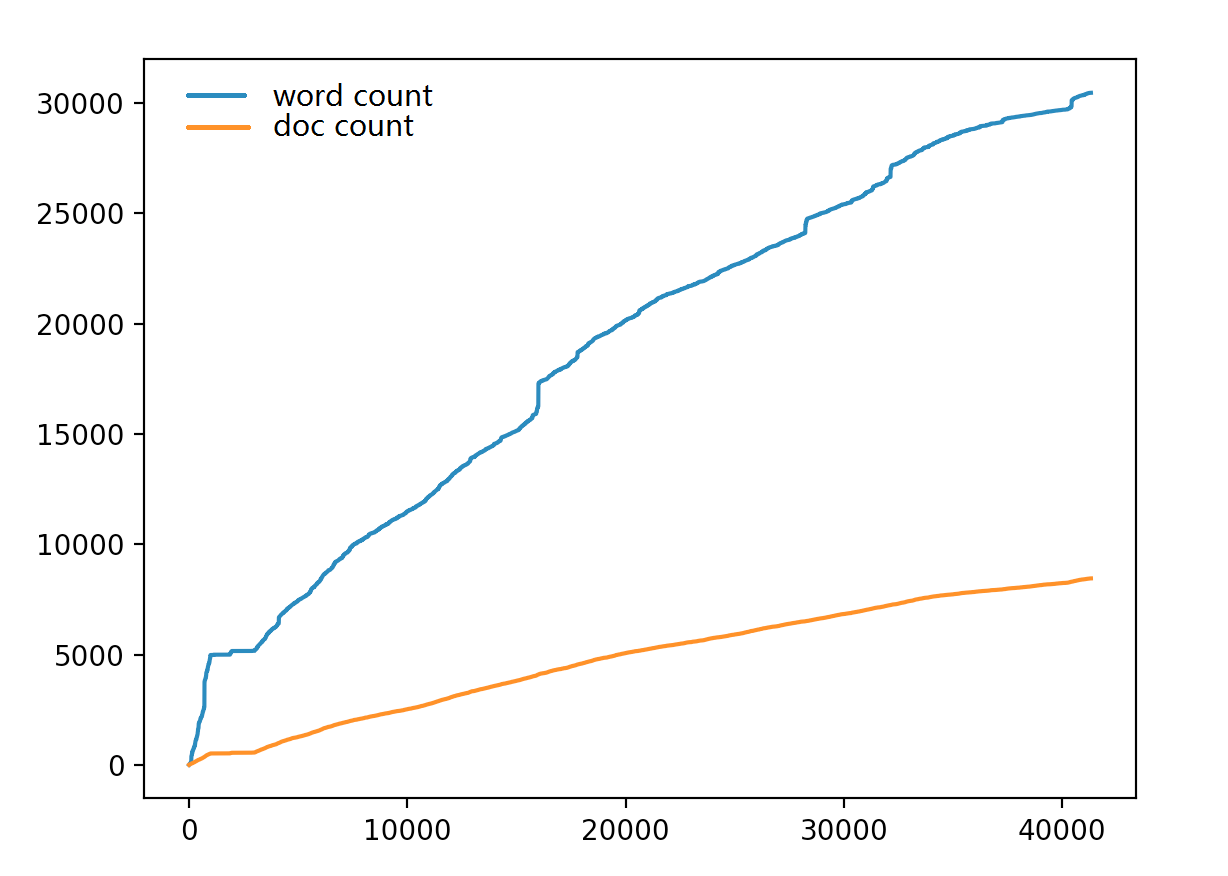
\includegraphics[width=0.5\linewidth]{noFreq2-5VsWords}
\caption{文档与低频词关系图}
\label{fig:noFreq2-5VsWords}       % Give a unique label
\end{figure}

图\ref{fig:noFreq2-5VsWords}中上方蓝色的线表示词频2-5的低频词随着文档数的增长趋势。下方的橙色线则表示包含这个区间内低频词的文档增长趋势。容易发现低频词的呈线性增长趋势。

通过前面章节的介绍,分布式主题模型的参数通常是一张词汇-主题计数表TAB(V, Z),表中的每一行对应着一个词汇的主题分布情况。
在流式环境下,由于词表是动态增长的,意味着如果想要保留新增的词汇,那么就必须维护一个动态词表。
在主题模型中,算法需要做到计数表TAB(V, Z)与词汇表表保持一致,
因而维护一个动态词表的同时也要维护计数表TAB(V, Z)。
最简单的方式便是当词表中新增一个词汇时,相应地创建一个新的主题计数向量。
同理如果删除一个词汇也要相应地删除这个主题的计数向量。

上面提及的简单的动态词表维护策略,显然在实际应用中是行不通的。
这种做法将会遇到如下问题:

(1) 词表表超大,当主题个数超多时参数规模将会巨大无比。

(2) 维护动态词表需要频繁的增删动态词表和词汇-主题计数表TAB(V, Z),这种维护代价将造成频繁的内存创建和回收,使得算法变得低效而无法被容忍,同时还会影响算法的稳定性。

解决和两个问题最为简单且行之有效的方法是使用先验知识提前设计一个静态的词表,
这个词表里面只包含最经常被使用的一小部分最高频的静态词汇(根据前面的分析,仅需要涉及数十万个词汇即可)。
这种方法,避免了动态词表的维护,并且大大减少了参数规模,在许多主题模型的实现中都得到了应用。

\begin{figure}[htb]\centering
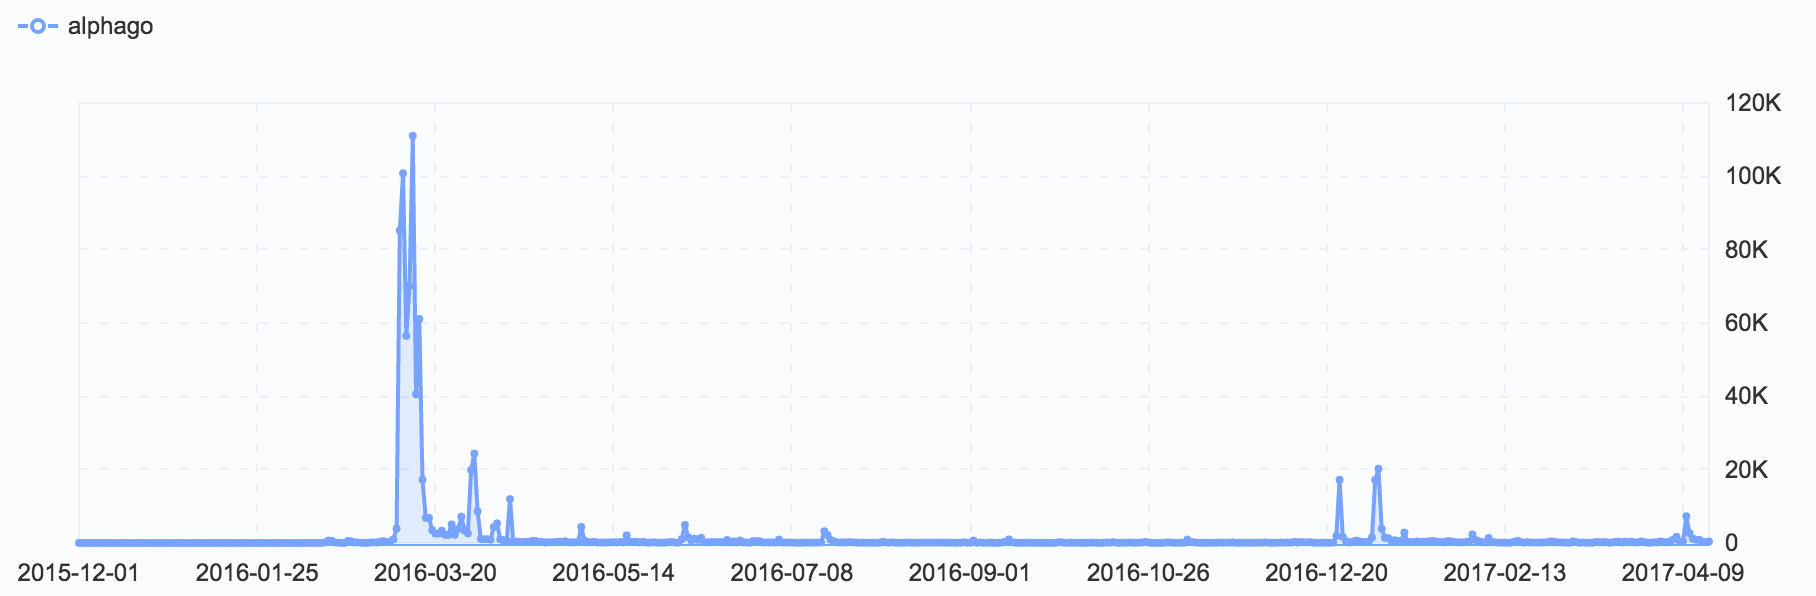
\includegraphics[height=0.23\linewidth,width=0.7\linewidth]{word-trend-alphago}
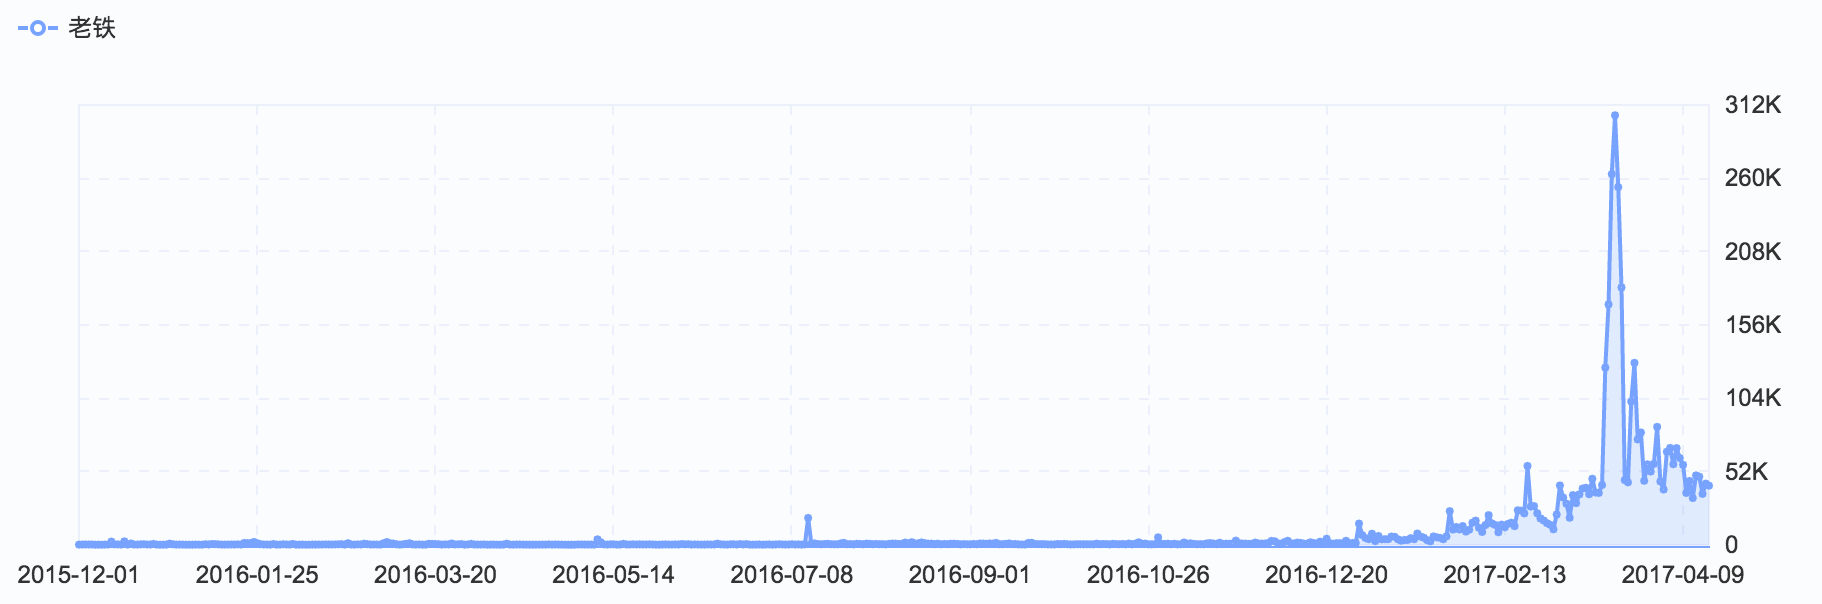
\includegraphics[height=0.23\linewidth,width=0.7\linewidth]{word-trend-laotie}
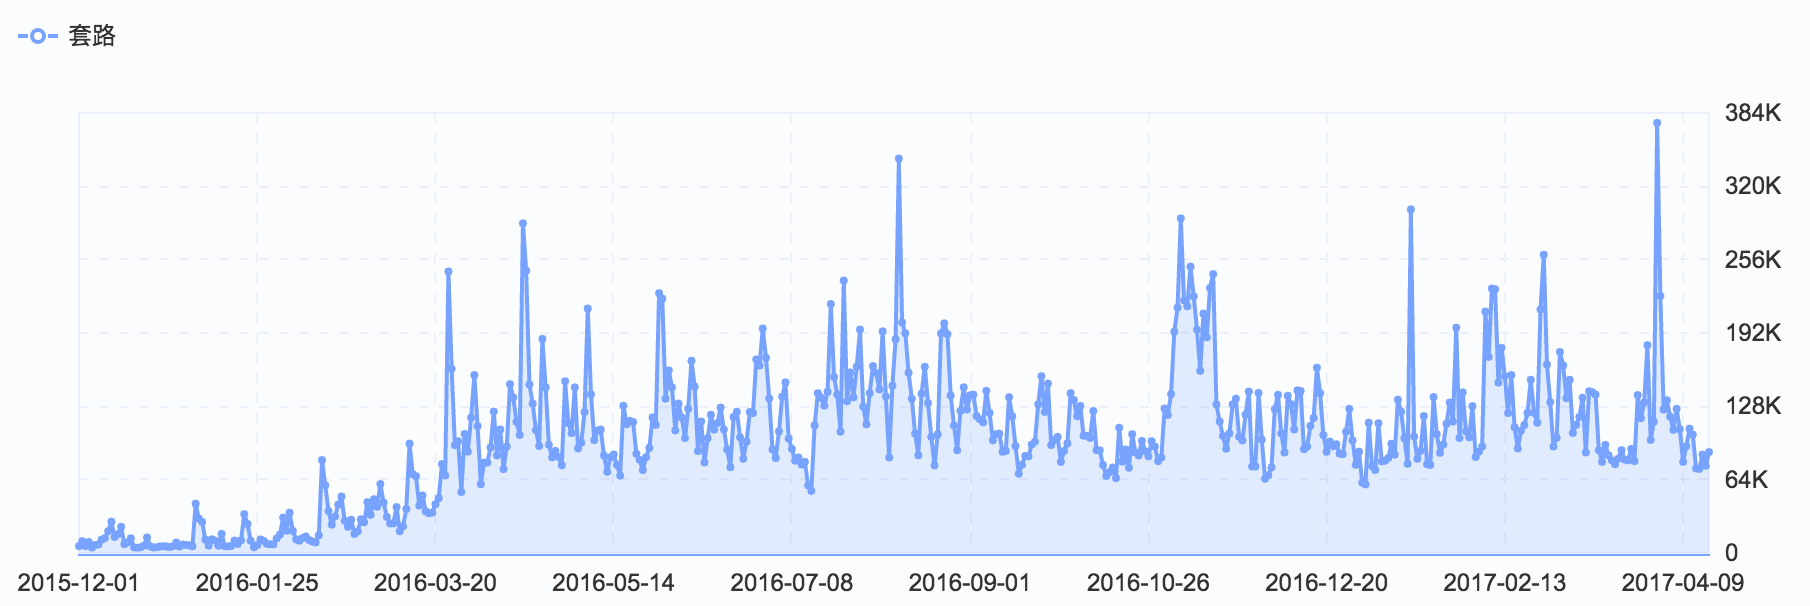
\includegraphics[height=0.23\linewidth,width=0.7\linewidth]{word-trend-taolu}
\caption{微博新词被提及的整体趋势}
\label{fig:new-word-trend}       % Give a unique label
\end{figure}

然而这种方法词表的规模很难确定,在不同的应用中主题模型可能需要不同阈值。
另外,固定大小的词汇表会使得许多有意义的词汇被忽略。
如图\ref{fig:new-word-trend}所示,“alphago”, “老铁”和“套路”均为近两年内新兴的词汇,并且被广泛使用。
这些词汇收到了广大网民的喜爱,具有鲜明的个性特征,对文本的语义具有决定性的作用,类似的词汇还有许多。
然而,这类新兴词汇也具有很强的时效性,在短暂的时间内被提及的数量会暴增,随着用户热情的退却又逐渐会退出舞台。
在筛选静态词表时,通常不具有被选到优势,因而有很大的概率会被忽略,这显然是一个重大的损失。

除此之外在具体的工业场景应用中,人们发现当数据量足够大且模型的主题个数足够多时,主题模型的效果会得到显著的提升。
这其中一个重要的原因是当数据量大时,许多覆盖低频词的主题语义被保留下来了\cite{Peacock}。
图\ref{fig:ntopics-pmi}显示了主题PMI分值,显然当主题个数越多时,PMI分值显著地提高了。

\begin{figure}[htb]\centering
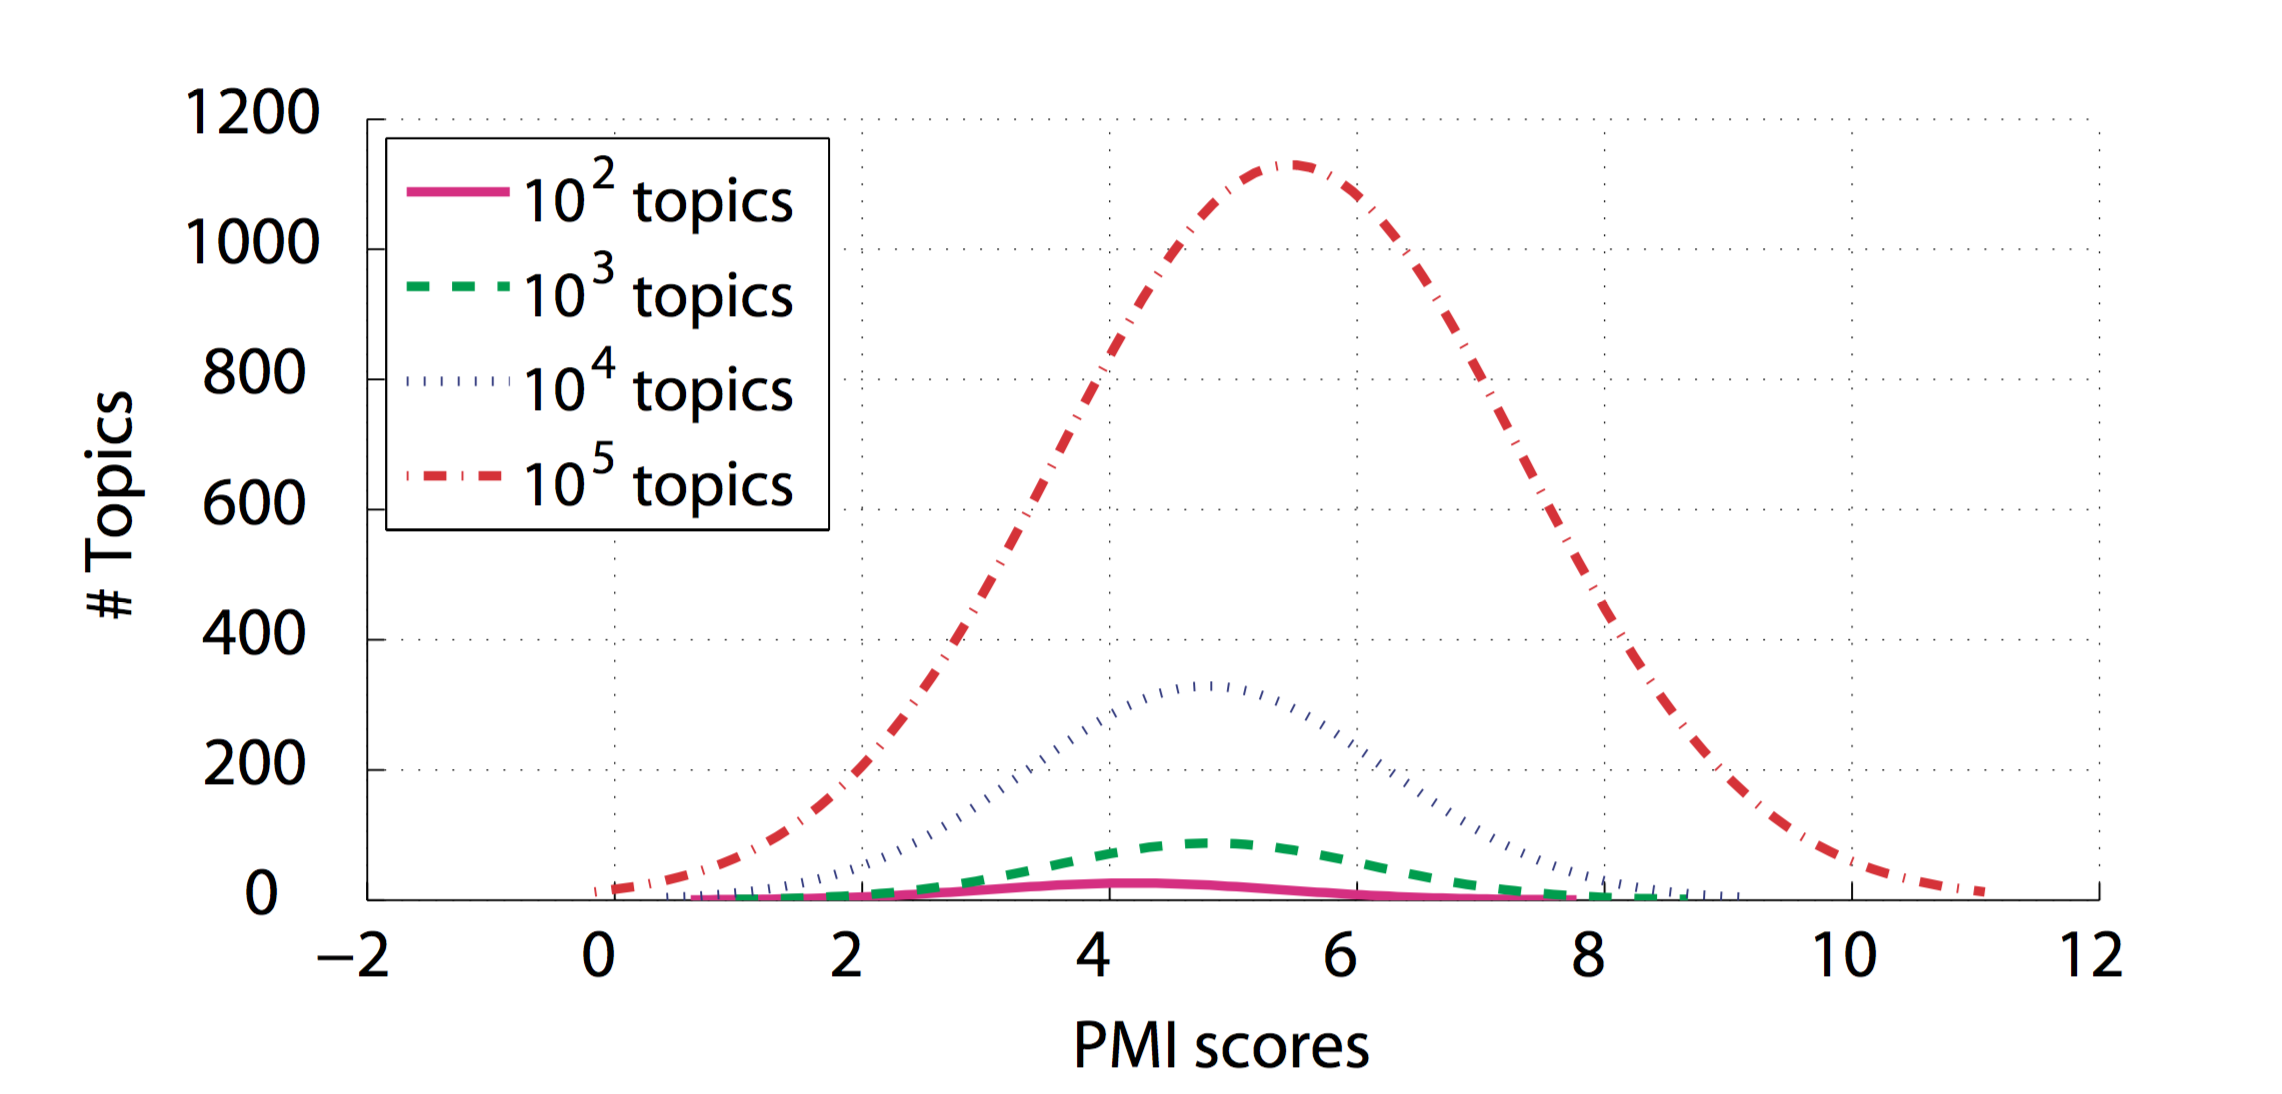
\includegraphics[width=0.7\linewidth]{ntopics-pmi}
\caption{LDA主题个数与PMI关系}
\label{fig:ntopics-pmi}       % Give a unique label
\end{figure}

这说明低频词在文本语义中并不是没有贡献的,恰恰相反低频词对模型效果的影响是显著的。
这些分析都说明在流式数据上维护一个动态词表具有重要的意义。

实际上许多地方都提到了主题模型的词汇-主题表TAB(V, Z)是一个特别稀疏的矩阵,对于大部分词汇来说,其语义是高度集中的,特别是低频词。
因而,如果采用稀疏表达的形式,比如哈希表,词汇-主题表的规模将大大减小。
然而完全使用稀疏表达也存在两个问题:

(1) 稀疏表达的矩阵或向量的随机访问效率不如稠密矩阵的高

(2) 当矩阵或向量相对稠密时,使用稀疏表达需要数倍于稠密的表达的空间消耗

上述的两个问题都会影响到主题模型算法的效率,其中第二个主要体现于在参数更新和访问过程中需要更多的网络传输。


\begin{figure}[htb]\centering
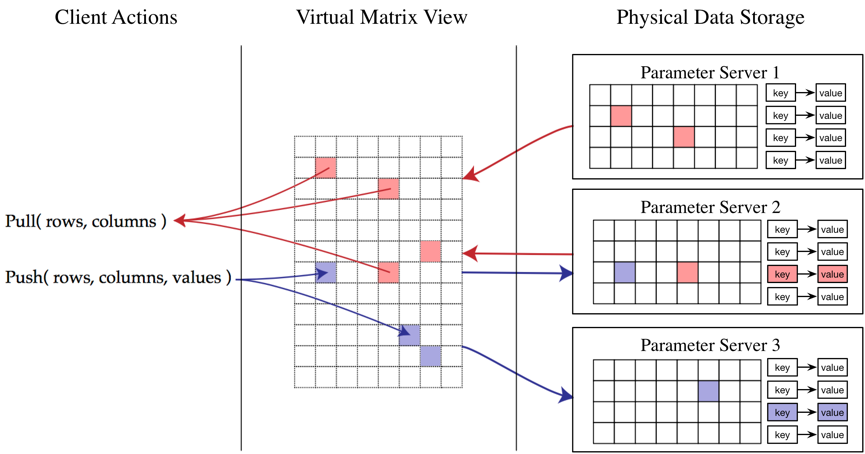
\includegraphics[width=0.8\linewidth]{hybrid-ps}
\caption{混合参数数据结构}
\label{fig:hybrid-ps}       % Give a unique label
\end{figure}

因而本文提出的解决方法是一种混合的参数数据结构。
这种混合数据结构既包含了稠密的表达,同时又包含了稀疏的表达。
混合参数数据结构的设计基于如下事实:

(1) 词汇表动态增长,无法提前预知词汇表大小

(2) 不到$10\%$的高频词,覆盖了$95\%$的语料

(3) 采用静态词表将会舍弃大量有意义的词汇(常见做法)

(4) 参数表$n(w,t)$是一个高度稀疏的表


在构建词汇表过程中,我们首先选取一个足够大的静态词汇表。
主要做法是选取一个相对较大的阈值筛选出了一部分高频词,针对这些词汇采用静态的词汇集表示。
剩余的词汇则采用动态的词汇表表示,由于数据流中不对会有新词出现,同时算法存在对过时的词汇的删除策略,因而动态词汇表时刻会产生变化。
针对静态词汇表,相应的主题模型参数采用了稠密的矩阵表示,并使用词汇ID索引。
针对动的态词汇表,相应的主题模型参数采用了稀疏的Hash存储,并使用词汇本身索引。
通过上面的设计方案,我们既高效地维护了一个动态词表,同时又使得绝大多数参数访问和修改发生在了稠密矩阵上。

如图\ref{fig:hybrid-ps},词汇-主题表所对应的参数结构按照词汇表的设计被划分成为了两个部分,
其中一部分是静态的稠密矩阵Dense(V, Z)表示,另外一部分则是使用<key, value>的形式进行稀疏表Sparse(V, Z)表示。

\section{参数数据结构的实现}
根据上面的参数数据结构的设计,在实现过程中我们还要考虑诸多因素。
在本文的实现中,我们使用了开源的glint\cite{glint}作为稠密参数的存储,使用了redis\cite{redis}内存键值缓存系统作为稀疏存储。
除此之外,在实现过程中我们还需要考虑到数值类型的选择,稀疏存储Sparse(V, Z)的稀疏性维护,参数系统的备份和恢复。

\subsection{使用int和float基本类型}
除了上面通过优化参数数据结构的方案来提高算法的参数服务器的使用性能之外,
一些具体的实现技巧也能大大提高算法的效率,这种思路在许多高效的算法实现中都能看到。

在基本类型中,最经常使用的整型int和浮点型float都只占用4个字节,而long和double类型通常占用8个字节。
这些类型的值域分别是:

int $\sim [-2147483648, 2147483647]$,

float $\sim [-3.4E(+/-)38, 3.4E(+/-)38]$, 

long $\sim [-9223372036854775808, 9223372036854775807]$,
	 
double $\sim [-1.7E(+/-)308, 1.7E(+/-)308]$。

int和float所能表示的范围和精度有限,当数据太大时可能造成溢出。
然而当参数规模足够大时,使用4字节类型和使用8字节类型之间将会有成倍的存储效率差距。

但是根据图\ref{fig:power-law}显示,除了静态词很少会有词汇超过int所能表达的值域。
l而在主题模型中静态词通常会在训练之前被遭到过滤。所以使用long和double类型意味着很大的浪费。

在本文的实现中,我们选择了4字节基本类型作为参数类型。

\subsection{稀疏存储Sparse(V, Z)的维护}
在本文主题模型参数数据结构的设计中,低频词-主题分布表Sparse(V, Z)的稀疏性起到了至关重要的作用。
但是如果没有得到维护,也会显现出一些问题。本节主要介绍流式环境下如何维护Sparse(V, Z)稀疏矩阵。

在上一章,本文介绍了在线流式主题模型\ref{alg:onlineStreamLDA}。

实际上在线流式主题模型中,参数$\beta^{(t)}(w, k) = (1 - \rho_t) \beta^{(t-1)}(w, k) + \rho_t n_{k, w}^{(t)}$是一个加权平均值。
其中$\rho_t \in (0, 1)$,说明几轮迭代之后,$\beta^{(t)}(w, k)$将会出现很多小数值。
假设$\beta^{(t-\sigma)}(w, k) = 1$,并且在其后的$\sigma$轮迭代中都有$n_{k,w} = 0$,
那么$\beta^{(t)}(w, k) = (1 - \rho_t)^{\sigma} > 0 $。
我们发现$\beta^{(t)}(w, k)$将会变得较小,但是不会变为0。
换句话说,$\beta^{(t)}$矩阵中将会出现大量的非零元,Sparse(V, Z)的稀疏性会大大降低,带来的是存储空间的消耗和更多的网络传输。

然而$\beta^{(t)}$中的绝大多数非零元对LDA Gibbs采样概率分布的影响微乎其微。
为了保证$\beta^{(t)}$的稀疏性,本文提出了两种做法:

(1) 设置阈值,对较小的小数进行截断。比如,如果$\beta^{(t)}(w, k) < 0.05$,删除该非零元。

(2) 采用int类型存储$\beta^{(t)}$,在每轮迭代的执行加权平均时使用四舍五入的方法转为整型。


\subsection{参数的备份和恢复}

对于一个长时间运行的系统,任务失败是一个很常见的事情。
\begin{table}\label{tab:jobs_failed} 
\center
\caption{某数据中心3个月机器学习任务统计}
\begin{tabular}{|r|r|r|}
\hline
$\approx$ \#machine $\times$ time & \# of jobs& failure rate \\
\hline
100 hours & 13,187 & $7.8\%$ \\
1,000 hours & 1366 & $13.7\%$ \\
10,000 hours & 77 & $24.7\%$ \\
\hline
\end{tabular}
\end{table}

论文\cite{li2014scaling}中统计了某数据中心3个月机器学习任务信息,表格显示随着算法规模的变大,任务出错的可能性也越大。

造成这些错误的原因多种多样,在流式主题模型中主要的原因可能有:
(a) 程序内部的BUG;(b) 算法运行超时;(c) 网络拥塞造成节点通信失败。

现有的分布式并行处理框架都有设计并提供容灾机制。
比如Spark中,如果一个Task失败之后,任务调度器还会尝试重启运行改Task。
本文的流式主题模型就是在Spark Streaming的计算框架下实现的。

然而Spark所提供的容灾机制并不能解决本文所提出的流式主题模型失败的问题。
主要原因在于,在流式主题模型运行采样过程中,算法会频繁地更新参数服务器上的参数。
虽然我们引入了许多优化方法,降低了模型参数的同步要求提高了并行度,但是在算法执行过程中参数服务骑上的参数始终维持一致性。
当错误出现时,部分参数将会丢失,系统会抛出任务失败信息,但是我们无法定位失败时程序执行的位置。
也就是说,参数服务器上的参数一致性受到了破坏。
在这种情况下,即使我们重启了Task,仍然无法恢复参数的一致性,因而继续执行算法仍然会持续失败。

为了提升算法系统的可用性,本文设计了参数的备份和恢复机制,如图\ref{fig:recovery}。
\begin{figure}[htb]\centering
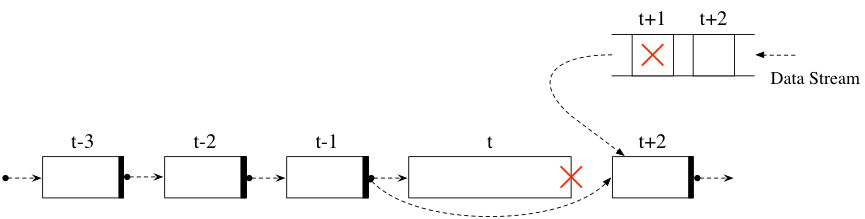
\includegraphics[width=1\linewidth]{recovery}
\caption{备份和恢复机制示意}
\label{fig:recovery}% Give a unique label
\end{figure}

\subsubsection{备份机制}
在本文的算法设计中,算法的参数在某些时刻是维持同步的,这些时刻包括每轮迭代之前和迭代完成之后的时刻。
虽然这些时刻都可以作为合理的参数被份节点,但是本文的算法实现中我们选择了流式数据每个时间片开始执行之前的时间节点作为参数备份节点。

我们知道,参数的备份是一个耗时耗空间的操作,并且在备份期间算法无法算法必须停止运行。
但是,为了维护系统的稳定性保证在失败时能够正确地重启算法,备份机制是必要的。
考虑到这些因素,流式数据的自然时间切片是一个较好的备份时间间隔。
在图\ref{fig:recovery}中每个时间片执行完成之后便会启动备份,虚线箭头左端的黑色区域表示备份阶段。
下一个时间片的算法之前参数需要与备份的参数保持一致。
这么做我们不仅能够更好地维持流式数据的动态变化模型,而且使得算法系统花在备份的时间空间相对较少。

\subsubsection{恢复机制}
根据前面的叙述,算法运行超时是算法执行失败的一个重要因素。
在真是应用场景中,由于流式数据的突发性特点,每个时间片的每个分区的算法运行时间很难得到有效的控制。
所以,超时是一个时常发生的事情。尽管如此,也并不是所有的超时都会引起失败。
那些引起失败的时间任务势必严重超时了。

在算法失败之后,为了保证系统继续运行,必须引入算法的恢复机制。
然而恢复机制的选择对系统的稳定性也有较大的影响。
一方面恢复是一个耗废资源的操作,并且在此期间算法也要停止运行;
另外一方面,即使正常恢复了算法运行,不同的恢复机制也对算法继续运行的鲁棒性有影响。

在前面提到的超时失败的问题中,如果算法直接从失败的位置恢复并继续运行,那么势必延长该时间片任务的执行时间。
那么,在严重超时的情况下,后续的时间片仍然需要等待当前时间片任务运行完成。
这是一个阻塞的过程,这种恢复机制只会造成算法稳定性的持续下降,并不是一个好的方式。

在本文提出的恢复机制中,我们秉持的调度原则是,当时间片到达时应该被第一时间处理。
如图\ref{fig:recovery}
当某一时间片的任务失败之后,那么该时间片将会被抛弃,同样被抛弃的时间片还会有其后续的未处理的时间片,最终只保留等待队列中的最后一个时间片并启动运行它。
这种方法使得算法消除了超时的负面影响,大大提高了算法的稳定性。
考虑到被丢失的数据,只会占整个数据流的很小的一部分,因而不会对算法模型的效果造成什么影响。

\section{实验分析}

\subsection{静态词表实验分析}
\begin{figure}[htb]\centering
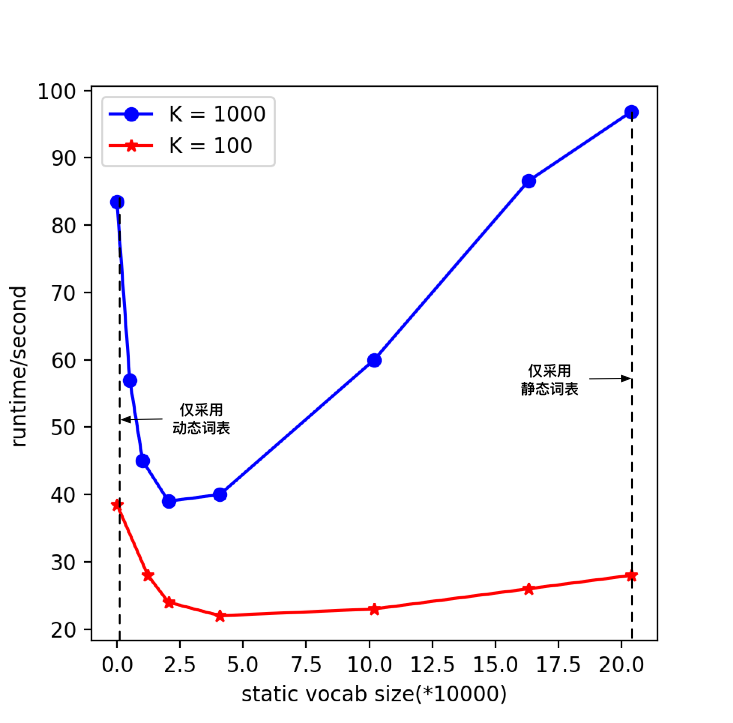
\includegraphics[height=0.41\linewidth]{static-vocab-vs-runtime}
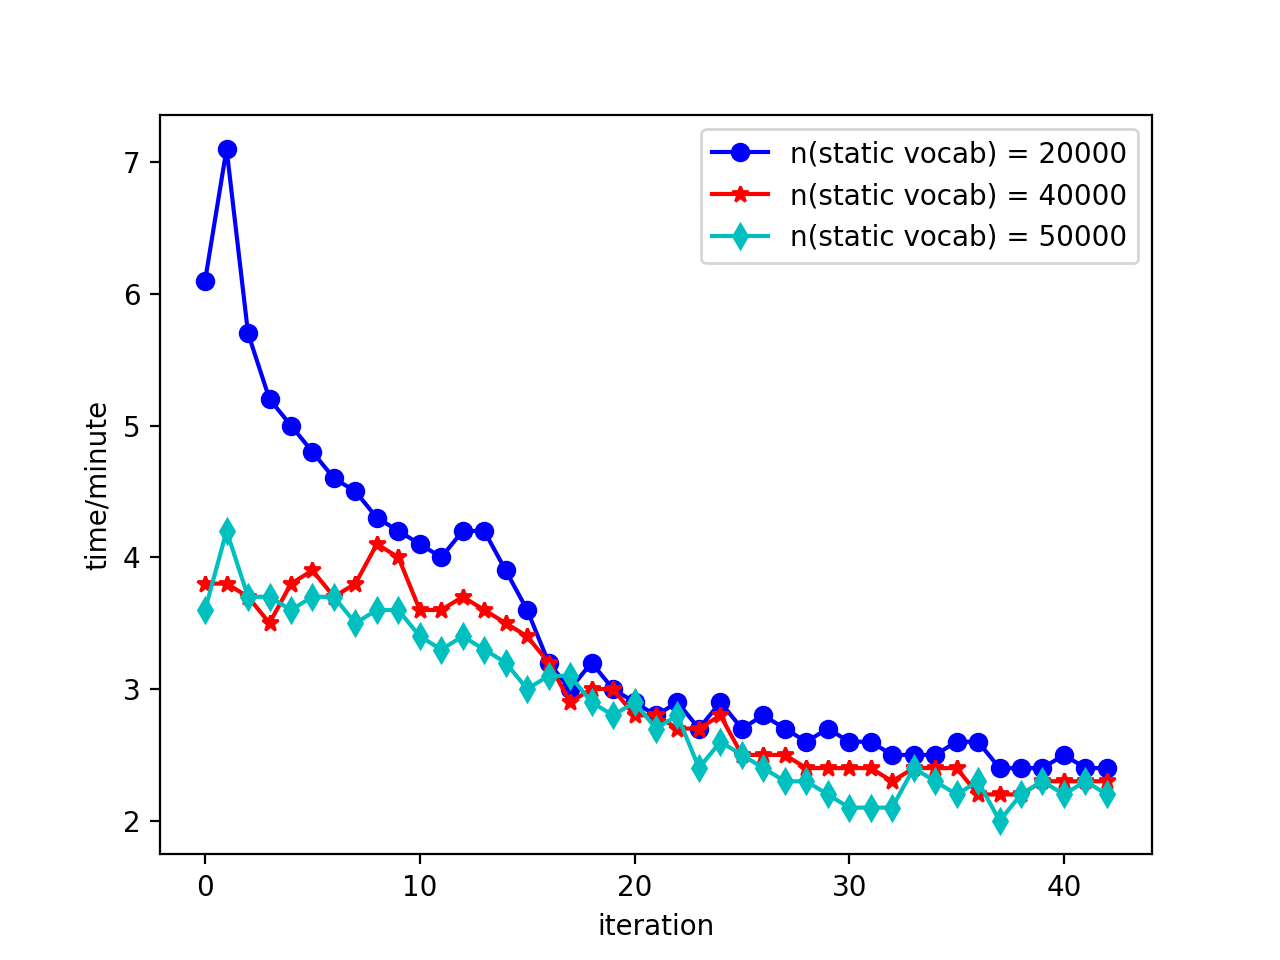
\includegraphics[height=0.41\linewidth]{static-vocab-runtime-iteration}
\caption{静态词表大小与运行时间关系示意}
\label{fig:static-vocab-runtime}       % Give a unique label
\end{figure}

图\ref{fig:static-vocab-runtime}所显示的是静态词表大小与算法运行时间之间的关系。

在左子图中,实验中每轮迭代遍历41310个文档,语料中出现的词汇总量为203891。
左子图中显示的纵坐标运行时间为算法采样10轮的时间平均值(单位为秒),横坐标表示的静态词汇表的大小(*10000)。
本文分别统计了主题维度为100和1000两种情况下,算法运行时间与静态词汇表大小之间的关系。
如图所示,我们不难发现曲线呈对钩形状。在这个实验中静态词汇表的带下设置为50000左右比较合适。
静态词汇表太大,低频词会逐渐增多,意味着混合参数中的Dense(V,Z)表会变得越来越稀疏,因而会大大降低算法的性能。
另外一方面静态词汇表也不能太小,语料中高频词的覆盖率占了绝大多数,小的静态词汇表无法充分地覆盖语料,使得许多参数访问被转向Sparse(V,Z),从而也会降低算法的性能。

在右子图中,实验中每轮迭代遍历808301个文档,语料中出现的词汇总量为982101。
纵坐标表示每轮迭代的运行时间(单位为分钟),横坐标表示算法的迭代轮数。
如果所示,本文分别设置了三组静态词表大小(20000,40000,50000),主题模型的维度都为1000。
不管静态词表的大小如何,随着迭代轮数的增长,运行时间都表现出下降的趋势。
起初三组实验算法运行时间存在明显的差异,其中静态词汇表大小为20000的实验显示运行时间远大于另外两组。
但是随着时间的推移,运行时间逐渐降低并且逼近另外两组。这是因为Sparse(V, Z)随着算法迭代轮数的增加越来越稀疏,带来了网络传输量的急剧下降。

\subsection{算法的可用性实验}
\begin{figure}[htb]\centering
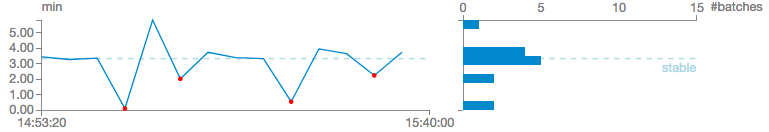
\includegraphics[width=1\linewidth]{stream-process-time}
\caption{Spark Streaming下流式主题模型的失败恢复实验}
\label{fig:stream-process-time}       % Give a unique label
\end{figure}
如上图所示,左子图为流式主题模型算法各批次运行时间图,右子图为运行时间的柱状图统计。
图\ref{fig:stream-process-time}中的虚线显示每个批次限定的合理运行时间为20000秒(3.3分钟)。
红色的点表示故障发生的时刻。可见故障发生后,算法重启具有一定的时延,但是都能够继续正常的运行。
通过左子图,我们还能够判断,除了少数超时和故障发生的情况,大部分时候算法维持稳定运行状态。
这得益于本文良好的算法设计。

\begin{figure}[htb]\centering
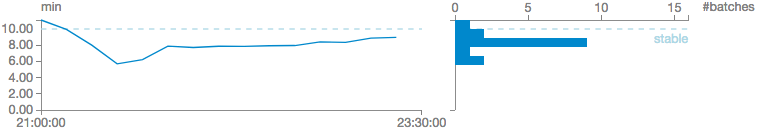
\includegraphics[width=1\linewidth]{stable-process}
\caption{流式主题模型运行状况示例}
\label{fig:stable-process}       % Give a unique label
\end{figure}

如图\ref{fig:stable-process}上图显示的是算法各个批次的运行时间,以及柱状统计图。
在参数设置合理的情况下,本文算能够持续鲁棒地运行。
在这个例子中,我们每个批次共输入50000篇文档,迭代15轮,主题个数为100,每个批次时间间隔10分钟。
我们发现除了算法开始执行的前几个批次算法运行时间超时外,其他批次的处理基本上不会超时。
并且,随着时间的推移每个批次的运行时间呈下降趋势,并最终稳定在8分钟左右。
这是因为在算法持续运行过程中,主题模型的参数逐渐变得稀疏,使得算法的运行效率有所提高。
并且当运行足够长时间之后,算法的稀疏性不会再有太大的变化。

\section{本章小结}
本章主要介绍了流式主题模型的参数结构设计。
在分布式并行算法实现中,人们通常会提及数据并行和模型并行两种并行方式。
参数服务器的出现,使得这两种并行方式能够更好地结合在一起。
在本文的算法实现中,我们应用了参数服务器作为分布式并行流式主题模型的主要组件。

在本章我们着重分析了流式数据环境下,动态增长的词汇表对主题模型实现所造成的影响。
并根据分析得到的结论提出了稠密和稀疏并存的参数数据结构。这种设计方案不仅有效地降低了参数存储的空间消耗,
还能够降低算法采样过程中的同步和更新所带来的网络消耗。

除了参数数据结构的设计,在本章中我们还介绍了,我们如何选择参数的数值类型和如何维护参数系数表Sparse(V, Z)的稀疏性。
在章节的最后,我们还指出了在流式环境下,算法系统因为多种原因所造成的失败。
为了保证算法系统的稳定性,本文提出了针对分布式流式主题模型的参数备份和恢复方案。
实验证明,本章提出的参数数据结构和容错机制能够保证算法高效和稳定运行。

\chapter{流式主题模型的采样算法}
\label{chapter:sample}
Gibbs采样算法是LDA模型估计参数的一种主要方法。
但是朴素的Gibbs采样算法复杂度偏高,会随着LDA主题维度线性增长。
流式数据环境对算法的实时性要求很高。对于一批数据的处理,如果时间过长,有可能造成超时,数据堆积等等不稳定因素,
严重时会造成系统奔溃。
因而,本文采用了Metropolis-Hasting算法与Alias Table结合的方法将每次采样的复杂度降低到了$O(1)$。
不仅如此,本文还在此基础上进一步对采样算法的采样顺序进行了调整,使得采样过程中的网络使用率进一步得到了提升。

\section{Metropolis-Hastings采样}
统计采样是个很常见的问题,通常在进行采样之前,我们都需要知道采样的来自的具体分布。但是,也有很多时候采样的分布的概率形式非常复杂,或者很难计算得到。
因而通过计算概率分布之后再进行统计采样的的方法也会遇到困难。
MCMC(Markov Chain Monte Carlo, MCMC)方法是解决这种问题的常见途径。

\begin{theorem}[马氏链收敛定理]
如果一个非周期马氏链具有转移概率矩阵$P$, 且任何状态是连通的,那么有:

1. $\lim_{n\rightarrow \infty} P_{ij}^n = \pi(j)$

2. $\pi(j) = \sum_{i = 0}^{\infty}{\pi(i)P_{ij}}$

3. $\pi$是方程$\pi P = \pi$的唯一非负解

4. $\sum_{i=0}^{\infty}{\pi_i} =  1$

称分布$\pi$为马氏链的平稳分布。

\end{theorem}

从任何初始概率分布$\pi_0$出发,我们在马氏链上做状态转移,记$X_i$的概率分布为$\pi_i$,则有:
\begin{align*}
X_0 \sim \pi_0(x) \\
X_1 \sim \pi_1(x) \\
... \\
X_n \sim \pi_n(x) = \pi(x) \\
X_{n+1} \sim \pi(x) \\
X_{n+2} \sim \pi(x) \\
\end{align*}

由马氏链收敛定理,概率分布$\pi_i(x)$将收敛到平稳分布$\pi(x)$。假设到第$n$步的时候马氏链收敛,我们得到$X_n, X_{n+1}, X_{n+2}, ... \sim \pi(x)$是服从于同一个分布的随机变量。
那么如果从一个具体的初始状态$x_0$开始,沿着马氏链按照概率转移矩阵做跳转,
那么我们得到一个转移序列$x_0, x_1, x_2, ..., x_n , x_{n+1}, ...$,由于马氏链的收敛行为,我们知道$x_n, x_{n+1}, ...$都是来自于平稳分布$\pi(x)$的观测值。
使用这个绝妙的方法,我们便得到了一组来自于$\pi(x)$分布的样本。

根据上面的介绍,我们知道了在马氏链收敛定理中一个很关键的因素便是转移矩阵$P$,所以MCMC的一个关键问题便是如何定义和构造转移矩阵$P$,使得我们能够得到平稳的分布$\pi(x)$。

\begin{theorem}[细致平稳条件]
如果非周期马氏链的转移矩阵$P$和分布$\pi(x)$满足
\begin{equation}
\pi(i) P_{ij} = \pi(j) P_{ji}\mbox{  for all }i,j
\end{equation}
\end{theorem}

显然根据上面的细致平稳条件,我们很容易得出:
\begin{align*}
\sum_{i=1}^{\infty}{\pi(i) P_{ij}} = \sum_{i=1}^{\infty}{\pi(j) P_{ji}}= \pi(j) \Rightarrow \pi P = \pi
\end{align*}

给定非周期马氏链以及概率分布$p(x)$,现在假设已经得到了一个转移矩阵$Q$,用$q(i \rightarrow j)$表示从状态$i$转移到状态$j$的概率,
通常细致平稳条件并不成立:
\begin{align*}
p(i)q(i\rightarrow j) \neq p(j) q(j \rightarrow i)
\end{align*}

为了得到快速得到一个满足细致平稳条件的马氏链,我们对原来的马氏链做一些修改。
比如,引入接受概率$\alpha(i -> j)$使得
\begin{equation}
\label{eq:accept}
p(i) \underbrace{q(i \rightarrow j) \alpha(i \rightarrow j)}_{q^{\prime}(i \rightarrow j)}= p(j) \underbrace{q( j \rightarrow i ) \alpha(j \rightarrow i)}_{q^{\prime}(j \rightarrow i)}
\end{equation}
为了使得式\ref{eq:accept}成立,最简单的方式便是令
\begin{align*}
\alpha(i \rightarrow j ) = p(j)q(j \rightarrow i), \alpha(j \rightarrow i) = p(i) q(i \rightarrow j)
\end{align*}

通过上面改造,我们顺利得到了一个满足细致平稳条件的新的非周期马氏链,令其转移矩阵为$Q^{\prime}$。因此马氏链$Q^{\prime}$的平稳分布便是$p(x)$。
这个过程可以通俗地理解为在原来的马氏链$Q$上,从状态$i$以概率$q(i \rightarrow j)$转移到状态$j$需要通过接受概率$\alpha(i \rightarrow j)$。
因而,$q(i \rightarrow j)$也被称为提议分布。

尽管如此,我们发现目前接受概率被定义为两个概率的乘积,可想而知得到的接受概率$\alpha(i \rightarrow j)$会是一个比较小的小数,那么有很大的概率会转移失败。
如果失败太多次的话,会严重影响收敛到平稳分布的速度。

为此我们可以同比放大两边的接受概率而不破坏细致平稳条件,令:
\begin{equation}
\alpha(i \rightarrow j) = \min\left\{ \dfrac{p(j)q(j \rightarrow i)}{p(i)q(i \rightarrow j)},1 \right\}
\end{equation}

于是经过上面的改造,我们得到一个接受概率较大的又满足细致平稳条件的马氏链。
这种做法被称为Metropolis-Hastings采样算法\ref{alg:metropolis-hasting}
\begin{algorithm}[htb]  
\caption{Metropolis-Hastings Sampling} 
\label{alg:metropolis-hasting} 
\begin{algorithmic}[1] 
\State Set initial state of markov chain $X_0 = x_0$
\For{t = 0, 1, 2, ...}
\State Sample $y \sim q(x_t \rightarrow y)$
\State Sample $u \sim Uniform[0,1]$
\State Set $\alpha( x_t \rightarrow y) = \min \left\{ \dfrac{p(x_t)q(y \rightarrow x_t)}{p(y)q(x_t \rightarrow y)}, 1\right\}$
\If{$u < \alpha(x_t \rightarrow y)$}
\State Accept $x_t \rightarrow y$
\Else
\State Reject $x_t \rightarrow y$
\EndIf
\EndFor
\end{algorithmic}  
\end{algorithm}  

\section{Alias Table}

Alias Table\cite{vose1991a}是一项生成随机数的技术。给定一个概率分布$p(X)$,Alias Table能够按照概率分布$p(X)$以$O(1)$的时间复杂度生成一个随机数$x$。
不妨令$p(X) = \{p_0, p_1, ..., p_n\}$表示在变量$X=\{X_0, X_1, ..., X_n\}$上的分布,其中$\sum_i^n {p_i} = 1, p_i \ge 0$。
那么Alias Table技术等价于一次$O(n)$复杂度的初始化操作和任意次$O(1)$复杂的随机数生成操作。

算法\ref{alg:alias-table}中prob和alias是在Init步骤构建好的两个大小为$n$的表。

\begin{algorithm}[htb]  
\caption{Alias Table} 
\label{alg:alias-table}
\textbf{\underline{Rand:}}
\begin{algorithmic}[1] 
\State $u = Uniform(n)$
\State $j = \lfloor u \rfloor$
\If { $(u - j) \le \mbox{prob}[j]$ }
\Return $j$
\Else
~~\Return $\mbox{alias}[j]$
\EndIf
\end{algorithmic}  
\textbf{\underline{Init:}}
\begin{algorithmic}[1] 
\State l = 0; s = 0
\For{ $j = 0\mbox{ to } n - 1$}
\If{ $p_j > \frac{1}{n}$}
$\mbox{large}[l] = j; l = l + 1$
\Else
~~$\mbox{small}[s] = j; s = s + 1$
\EndIf
\EndFor
\While{ $s\ne 0\mbox{ and }l \ne 0$}
\State $s = s - 1; j = \mbox{small}[s]$
\State $l = l - 1; k = \mbox{large}[l]$
\State $\mbox{prob}[j] = n \times p_j$
\State $\mbox{alias}[j] = k$
\State $p_k = p_k + (p_j - \frac{1}{n})$
\If{ $p_k > \frac{1}{n}$}
$\mbox{large}[l] = k; l = l + 1$
\Else
~~$\mbox{small}[s] = k; s = s + 1$
\EndIf
\EndWhile
\While{ $s > 0$}
$s = s - 1; \mbox{prob}[\mbox{small}[s]] = 1$
\EndWhile
\While{ $l > 0$}
$l = l - 1; \mbox{prob}[\mbox{large}[l]] = 1$ \EndWhile
\end{algorithmic}  
\end{algorithm}  

Init算法实际上是对一个面积为1的区域进行填空的过程。
这种填空方法的思路主要来自于,如果把概率看做长度,变量的宽都为1,
对于均匀分布有所有变量的长度都为$\frac{1}{n}$,刚好组成一个面积为1的矩形区域。
相当于将面积1等分为$n$个区间,此时随机选取一个$(0, 1)$之间的值,便能立即确定其属于哪个区间。
但这只是特例,大多数时候有一部分变量的概率不到$\frac{1}{n}$,而另外一部分概率超过了$\frac{1}{n}$,
为了构造上面提到的矩形,Alias Table的算法采取优先填满每个等分区间(每个区间最多被两个随机数占用)的方式,用长板补短板,逐一填空。

\begin{figure}[htb]\centering
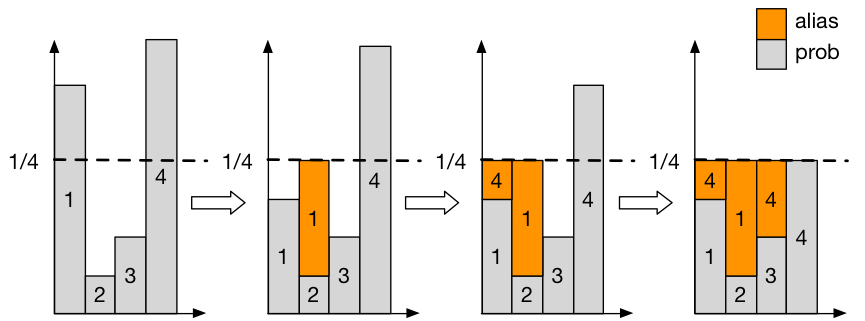
\includegraphics[width=0.8\linewidth]{alias-table}
\caption{Alias Table构建过程示意}
\label{fig:alias-table}       % Give a unique label
\end{figure}

如图\ref{fig:alias-table}, 实际上算法\ref{alg:alias-table}的Init步骤等价于在填写一个面积为1的矩形区域。

(1) 该矩形被等分为$n$份,每一份的面积等于$\frac{1}{n}$。

(2) 等分的$n$个子区域又各自分为prob和alias两部分,也就是$\mbox{len}(\mbox{prob}[i]) +\mbox{len}( \mbox{alias}[i]) = \frac{1}{n}$对于任意$i$都成立。

(3) 对于每个变量$X_i$,面积占比为$\mbox{area}[i] = \mbox{len}(\mbox{prob}[i]) + \sum_{j, alias[j]=i}{\mbox{len}(\mbox{alias[j]})}$。

(4) 对所有变量$X_i$,有$\mbox{area}[i] = p_i$。

\section{主题模型采样算法}
前面的章节已经简略地介绍了主题模型的Gibbs采样参数估计方法,Gibbs采样算法是Metropolis-Hastings算法接受概率为1的一个特例。
在LDA模型中我们会关心主题变量$z$在语料上的分布,然而我们事先并不知道$p\mathbf{ (z, w)}$的具体情况。
我们已经知道了通过MCMC方法可以收敛得到一些来自于某一稳定分布的样本。
为了应用MCMC来对LDA模型中的主题变量进行抽样,关键问题在于如何构建非周期性马氏链。
\begin{equation}
\label{eq:stable-cond}
p(z_i = x , \mathbf{z}_{\neg i}, \mathbf{w}) p( z_i = y | \mathbf{z}_{\neg i},  \mathbf{w})  =  
p(z_i = y , \mathbf{z}_{\neg i}, \mathbf{w}) p( z_i = x | \mathbf{z}_{\neg i},  \mathbf{w}) 
\end{equation}

根据公式\ref{eq:stable-cond},令$p( z_i = k | \mathbf{z}_{\neg i},  \mathbf{w})$为第$i$维的变量状态之间的转移概率,
那么在这个维度上各个状态之间的转换满足细致平稳条件。
现假设,LDA模型某一轮迭代的输入语料中有$M$个文档,文档的平均长度为$\bar{L}$,主题模型设定的主题变量个数为$K$。
那么Gibbs采样算法迭代一轮的时间复杂度为$O(M\times \bar{L} \times K)$,其中一次采样的复杂度为$O(K)$。
也就是说,随着主题模型变量个数的增大,模型的时间消耗随着线性增长。这种采样复杂度的效率较低,尤其在实时性要求高的环境中很难被应用。

\subsection{高效的提议分布}
实际上,造成Gibbs采样算法低效的主要原因是采样概率的计算比较复杂,并且需要被频繁地更新(每次采样之后都会得到更新)。
针对Gibbs采样算法效率低的问题,Sparse LDA利用了参数的稀疏性,将每次采样的算法复杂度降低到了$O(K_w)$。
Alias LDA算法同样利用了参数的稀疏性,但是引入了Metropolis-Hastings和Alias Table技术,将算法复杂度降低到了$O(K_d)$。
Light LDA同样应用了Metropolis-Hastings和Alias Table技术,将每次采样的算法复杂度降低到了$O(1)$,
但是这种方法需要交替地应用两种不同的提议分布,
以达到更好的收敛效果。
受到这些技术的启发,本文也提出了一种高效的采样算法。

我们发现,Metropolis-Hastings算法并不要求接受概率必须为1,并且对提议分布$Q$的定义也没有严格的要求。
提议分布$q(\cdot)$的选择对算法快速收敛到真实后验分布$p(\cdot)$具有重要的意义,
挑选得好的分布能够从两个方面提升采样效率:

(1) 从提议分布$q(\cdot)$中采样的效率要远远高于原分布$p(\cdot)$

(2) 非周期马氏链会迅速收敛到平稳状态

事实上,提议分布$q(\cdot)$的选择也是一个权衡利弊的过程。提议分布$q(\cdot)$和真实分布$p(\cdot)$越接近,则非周期马氏链收敛越快,
但是这么一来从$q(\cdot)$中采样可能和直接从$p(\cdot)$中抽样同样复杂。
反过来,如果选择一个不那么相似的提议分布$q(\cdot)$可以使得从$q(\cdot)$分布中采样效率非常高,但是马氏链收敛的速度可能会变极慢。

%本文中的采样算法采用了LightLDA中提及的Metropolis-Hastings方法。
%LightLDA拥有两个提议分布,并且交替地作为高效率的采样分布。

%在公式\ref{eq:sample-prob}中,第一项与文档主题计数$n_{k,d}$有关而与词汇主题计数$n_{k,w}$无关,
%另外一项则只和词汇主题计数$n_{k,w}$相关而与文档主题计数$n_{k,d}$无关。
%不难推理出,该采样公式中概率密度主要集中在那些词汇主题计数$n_{k,w}$和文档主题计数$n_{k,d}$都比较大的主题。
%因此,公式\ref{eq:sample-prob}两项均可以作为较好的主题采样分布的提议分布。

在公式\ref{eq:sample-prob}中,Gibbs采样分布与文档主题计数$n_{k,d}$和词汇主题计数$n_{k,w}$密切相关。
前面已经提到,造成Gibbs采样算法低效的一个重要原因是采样分布需要被频繁地更新。
然而,许多研究发现在短时间内主题的计数并不会发生巨大的改变。
尤其在流式数据环境下,本文提出的在线和增量流式主题模型方法中,受到主题分配词汇概率的Dirichlet先验,
每个时间片上的数据变动,对整体模型的影响进一步得到了约束。

本文提出的采样算法充分利用了上面提到的主题模型的特性。

\textbf{提议分布:}
\begin{equation}
 p_c(k) \propto p_w(k) p_d(k)
\end{equation}
其中:
\begin{equation}
\begin{aligned}
& p_w(z = k) \propto \dfrac{n_{k,w} +\eta}{n_{k, \cdot} + V \eta} \\
& p_d(z = k) \propto (n_{k,d} +\alpha) 
\end{aligned}
\end{equation}

\textbf{从状态$s$转移到$t$的接受率为:}
\begin{equation}
\begin{aligned}
& \alpha_c(z=k) = \min \left\{\dfrac{p(t) p_c(s)}{p(s)p_c(t)}, 1\right\} \\
& \dfrac{p(t) p_c(s)}{p(s)p_c(t)}= \dfrac{ (n_{t,d}^{\neg di} + \alpha)(n_{t,w}^{\neg di} + \eta) (n_{s,\cdot}^{\neg di} + V \eta) p_c(s)}
{ (n_{s,d}^{\neg di} + \alpha)(n_{s,w}^{\neg di} + \eta) (n_{t,\cdot}^{\neg di} + V \eta)p_c(t)}
\end{aligned}
\end{equation}

在上面的式子中,$n_{k,w}, n_{k, d}, n_{k, \cdot}$表示某一时刻主题模型参数中的相应值。
根据前面的分析假设,这些值在短时间内不会发生大的变化。
因而,分布$p_c(k)$与原采样分布$p(k)$比较相似,可以作为一个很好的提议分布。

本文设计的算法在每轮迭代中只会计算一次$p_w(k)$,对于每个文档只会计算一次$p_c(k)$。
然后执行预处理得到Alias Table,借助这项技术算法需要$O(K)$时间复杂度的预处理,但是每次采样只需要$O(1)$时间。
不仅如此,我们接受概率$\alpha_c(k)$的复杂度为$O(1)$,计算代价很低。
通过分析,不难发现算法执行一轮迭代的时间复杂度为$O(M \times \bar{L} + M \times K + W \times K)$,相比于原先的$O(M \times \bar{L} \times K)$。
不仅如此,我们发现$p_w(k)$和$p_d(k)$其实是两个高度稀疏的向量,借助这个特性,我们可以将采样的复杂度进一步降低到$O(M \times \bar{L} + M \times K_d + W \times K_w)$。


\subsection{优化算法采样顺序}

\begin{algorithm}[htb]
\caption{Sample in Natural Order}
\label{alg:natural-order}
\begin{algorithmic}[1] 
\Require TAB(V, Z), $\mathbf{k} = [1, 2, ..., K], \mathbf{w}$
\For { m = 1 to $M$ }
\For { n = 1 to $N_m$}
\State \textbf{Require} parameter $n(w_{mn}, \mathbf{k}) \sim$ TAB(V, Z)
\State SAMPLE($z_{mn}, n(w_{mn}, \mathbf{k})$)
\EndFor
\EndFor
\end{algorithmic}  
\end{algorithm}  
常见的主题模型Gibbs采样算法是坐标轴下降方法,交替轮换坐标轴逐一地采样更新。
在一般情形中,对语料采样通常是语料中词汇出现的自然顺序,先后地对出现的词汇执行采样,如算法\ref{alg:natural-order}。

\begin{algorithm}[htb]
\caption{Sample in Vocabulary Order} 
\label{alg:vocab-order}
\begin{algorithmic}[1]
\Require TAB(V, Z) = \textbf{\{Dense(V, Z), Sparse(V, Z)\}}, $\mathbf{k} = [1, 2, ..., K], \mathbf{w_d, w_s}$
\Function{DO\_SAMPLING}{$\mathbf{n(v_b, k), w}$}
\For { each $(m , n)$ where $w_{mn } \in \mathbf{v_b}$}
\State SAMPLE($z_{mn}, n(w_{mn}, \mathbf{k}), \mathbf{w}$)
\EndFor
\EndFunction
\For { each block $\mathbf{n(v_b, k)}$ in \textbf{Dense(V, Z)} }
\State Issue DO\_SAMPLING($\mathbf{n(v_b, k), w_d}$)
\EndFor
\State Set $\mathbf{v_s}$ as the low-frequent vocabulary local
\State Pull all $\mathbf{n(v_s, k)} \sim $ \textbf{Sparse(V, Z)}
\State Issue DO\_SAMPLING($\mathbf{n(v_s, k), w_s}$)
\end{algorithmic}  
\end{algorithm}  

根据LDA模型Gibbs采样的概率分布公式,词汇采样过程中将会使用到与词汇关联的词汇主题分布$n(w, \mathbf{k})$。
但是自然顺序,词汇在语料中的分布式散乱的,前后被采样的词汇基本上是不相同的,相当于每次采样都随机地访问了词汇-主题表TAB(V, Z)中的一行。

这种情况下词汇主题分布向量$n(w, \mathbf{k})$难以被复用(做到这点必须完全加载整张表,而前面分析提到这张表有可能超过单机内存的容量)。
另外一方面,如果不复用$n(w, \mathbf{k})$,则需要频繁地对参数服务器发起pull请求,这显然会增加网络请求的次数,
不仅产生了更多网络延迟同时也更容易造成参数服务器的响应瓶颈,更严重的情况可能造成参数服务器崩溃或者网络通信失败。
显然,这种访问效率是极其低效的。

实际上,Gibbs采样算法并没有严格要求采样的顺序。
根据主题模型参数数据结构的设计,令TAB(V, Z) = \{Dense(V, Z), Sparse(V, Z)\},
其中Dense(V, Z)表示稠密的参数矩阵,Sparse(V, Z)表示稀疏的<Key, Value>参数矩阵。

Dense(V, Z)所对应的词汇子集都是高频词,这些词汇在所有语料子集上都有很大的概率会出现。
根据这些特性,按块读取稠密矩阵Dense(V, Z),虽然有可能会下载一些无用的参数,但是将会大大提高网络传输的效率。

Sparse(V, Z)所对应的词汇子集含有大量的低频词,大部分词汇不大可能出现在所有的语料子集上。因而每个子集上的低频词词汇表只是全局低频词词汇表的一个较小的子集
。因为这部分参数高度稀疏,所以实际中可以完整下载本地所有需要的参数。

根据以上的参数数据结构特性,本文算法\ref{alg:vocab-order}实现中将文档分为高频词和低频词两部分。
之后对高频词部分按照词汇表顺序排序汇总。
同时对静态稠密的Dense(V, Z)参数矩阵进行分块。

当采样算法开始时,算法实现按照块读取的方式读取Dense(V, Z)参数稠密矩阵的一部分,并在语料文档中的稠密部分执行相应词汇的重采样。
执行完改步骤之后,从Sparse(V, Z)中pull将本地所有本地需要的低频词参数,并执行文档低频词部分的重采样。

\subsection{Pipeline参数更新}
当Gibbs采样是按照文本语料中词汇的自然顺序采样时,参数不得不等待所有语料中词汇都被采样之后在同步更新。
这种做法在采样过程中网络处于空闲状态,而在参数更新时又很容易出现网络使用高峰。

在按照上一小节的方式优化Gibbs采样顺序之后,我们发现每个词汇的主题分布向量无需互相等待,因而在一个词汇所有出现位置都经过采样之后便可以执行参数的增量更新。
这种方法称之为Pipeline,它将参数在时间维度上异步均摊地执行网络更新,不仅在采样过程中利用了网络,还有效地解决了网络高峰的问题。

\begin{figure}[htb]\centering
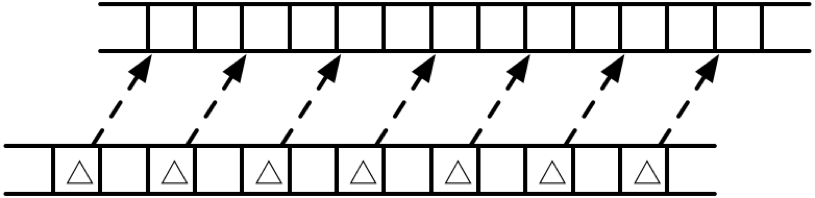
\includegraphics[width=0.7\linewidth]{pipeline}
\caption{Pipeline异步地进行网络传输}
\label{fig:pipeline}       % Give a unique label
\end{figure}


\begin{algorithm}[htb]
\caption{Pipeline Parameters Update} 
\label{alg:pipeline}
\begin{algorithmic}[1]
\Require TAB(V, Z) = \textbf{\{Dense(V, Z), Sparse(V, Z)\}}, $\mathbf{k} = [1, 2, ..., K], \mathbf{w_d, w_s}$
\Function{DO\_SAMPLING}{$\mathbf{n(v_b, k), w}$}
\For { each $(m , n)$ where $w_{mn } \in \mathbf{v_b}$}
\State GibbsSampling($z_{mn}, n(w_{mn}, \mathbf{k}), \mathbf{w}$)
\State Calculate update $\Delta \beta(w, \mathbf{k})$
\EndFor
\State Push $\Delta \beta(\mathbf{v_b}, \mathbf{k})$ to parameter
\EndFunction
\For { each block $\mathbf{n(v_b, k)}$ in \textbf{Dense(V, Z)} }
\State Issue DO\_SAMPLING($\mathbf{n(v_b, k), w_d}$)
\EndFor
\State Set $\mathbf{v_s}$ as the low-frequent vocabulary local
\State Pull all $\mathbf{n(v_s, k)} \sim $ \textbf{Sparse(V, Z)}
\State Issue DO\_SAMPLING($\mathbf{n(v_s, k), w_s}$)
\end{algorithmic}  
\end{algorithm}  

\section{实验分析}
\subsection{采样算法效率分析}

本节首先对本文提出的Metropolis-Hastings采样方法的效率进行实验设置。
\begin{figure}[htb]\centering
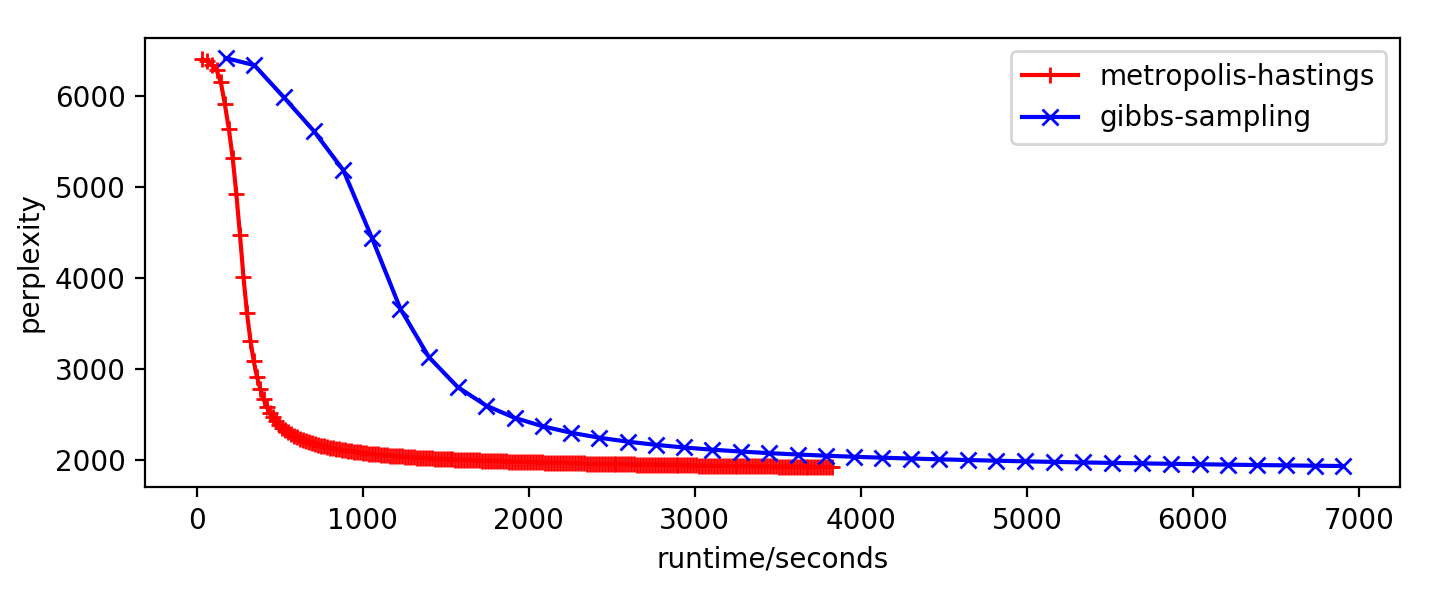
\includegraphics[width=1\linewidth]{exp-mh-vs-gibbs-perplexity-runtime}
\caption{本文Metropolis-Hastings方法与Gibbs采样算法效率对比}
\label{fig:mh-vs-gibbs}       % Give a unique label
\end{figure}

如图\ref{fig:mh-vs-gibbs},在实验中本文选取的Gibbs采样实现为GibbsLDA++\cite{gibbsLda++}。
为了更好地进行采样算法的效率对比,本文选取的主题模型训练法方式是在静态数据集上的批量学习方法。
在这个实验中,本文选取的语料中共有119301篇文档,53893799个词项;
主题模型的参数设置分别为$\alpha = 0.5, \eta = 0.01, K = 100$;
选取的评价指标为Perplexity。图中每个标记点均为一次迭代得到的Perplexity评估值。

通过对比,我们不难发现,Gibbs采样算法仅需要更少的迭代次数便能接近收敛,
但是本文提出的Metropolis-Hastings算法比Gibbs采样的收敛要更快。
这主要体现在Metropolis-Hastings算法采样的效率更高,迭代速度更快。
在实验过程中,我们发现Gibbs采样算法每轮迭代的平均时间消耗为180秒左右。
而本文的采样算法每轮迭代仅需要20秒。
事实上,如果我们将主题模型的主题个数$K$增大,这种差距会更加明显。

\subsection{算法网络效率分析}

本节实验主要从网络效率的角度分析本文采样算法的效率。
\begin{figure}[htb]\centering
\begin{subfigure}{1\textwidth}
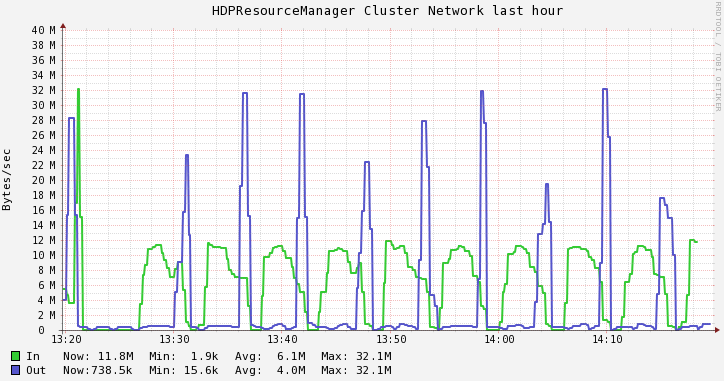
\includegraphics[width=0.75\linewidth]{exp-pipeline-hsq-network-1}
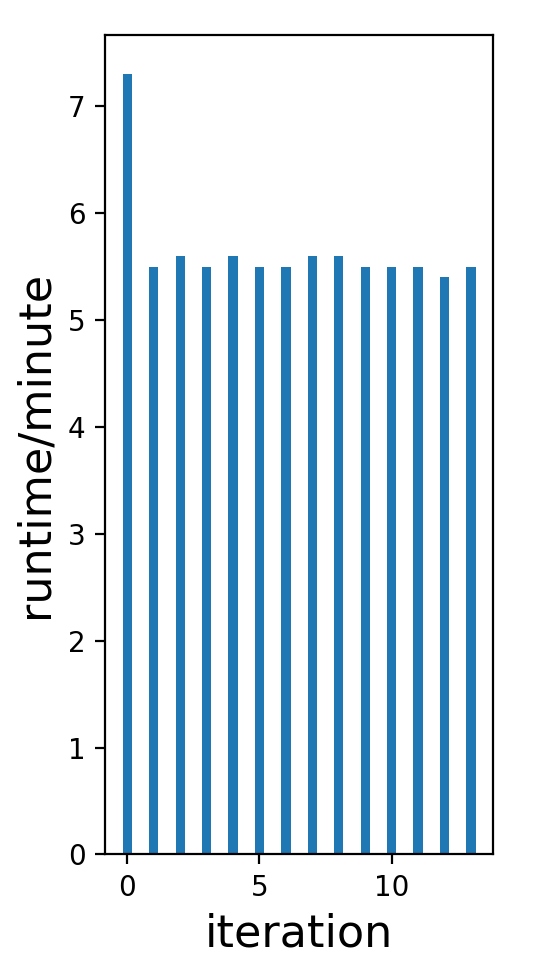
\includegraphics[width=0.23\linewidth]{exp-pipeline-hsq-runtime-1}
\caption{算法运行过程中未使用采样优化}
\end{subfigure}
\begin{subfigure}{1\textwidth}
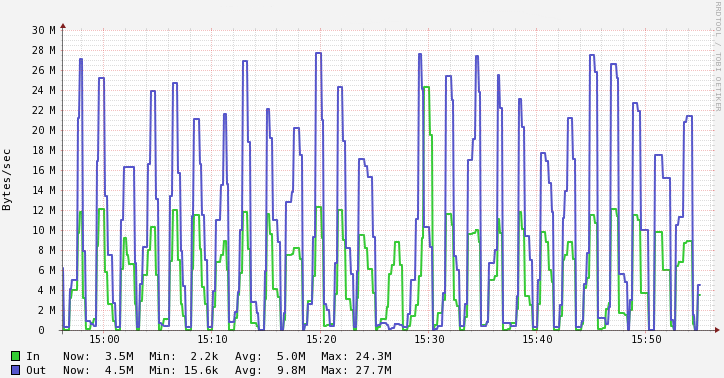
\includegraphics[width=0.75\linewidth]{exp-pipeline-hsq-network-2}
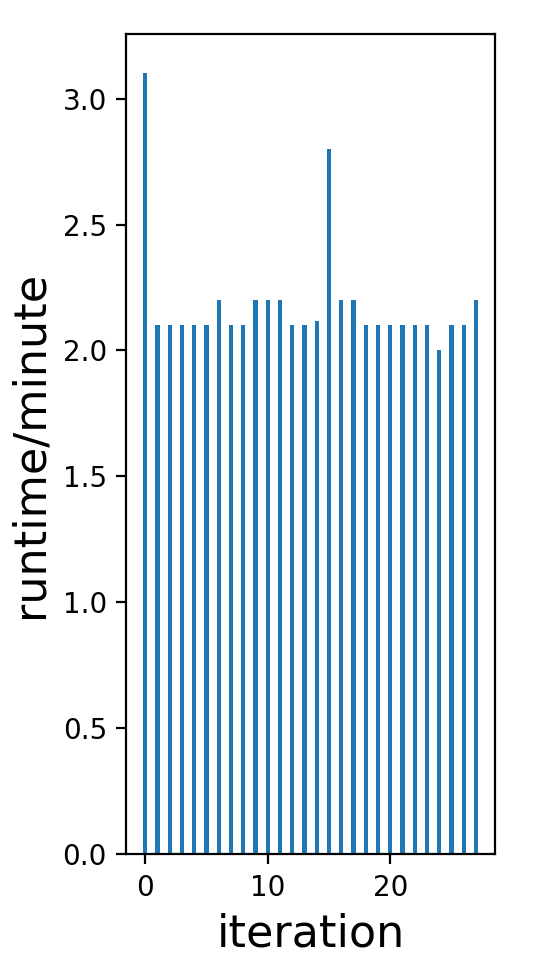
\includegraphics[width=0.23\linewidth]{exp-pipeline-hsq-runtime-2}
\caption{算法运行过程中使用了采样优化}
\end{subfigure}
\caption{采样算法的网络效率分析}
\label{fig:exp-pipeline}       % Give a unique label
\end{figure}

如图\ref{fig:exp-pipeline},在这两组实验中我们分别选择了是否进行采样优化,包括优化采样顺序和Pipeline更新。
两组实验中,左图为算法的网络流量图,右图为算法的迭代执行效率图。
网络流量图中,本文收集了算法迭代运行过程中的实时输入和输出网络流量,其中浅绿色峰值较小的是输入流量,深蓝色峰值较高的为输出流量。
造成输出流量波峰较高的原因主要是,输入流采样块读取机制,输出流采用随机索引更新的方式,造成了输出流的网络利用率更低。

通过对比两组实验,我们不难发现(a)组实验中输入流和输出流的的波峰明显是相互错开的,而(b)组实验中波峰是重叠在一起的。
事实上每个波峰对应着一次迭代,说明了(a)组实验的网络效率更低并且有巨大的延迟。
我们还发现,(b)组实验中几乎所有时刻网络都不存在空闲,平均网络的负载更大,但是网络峰值较低。
通过右图中的算法的执行迭代效率的对比也不难发现,两组实验的算法运行效率有着成倍的差异。
这个实验足以证明本文提出的采样算法优化不仅使得网络的利用更加充分、均衡,而且大幅提升了采样算法的效率和性能。

\section{本章小结}
Sparse LDA利用了主题模型参数的稀疏性来降低了采样的复杂度,
提出了一种Metropolis-Hastings和Alias Table相结合的新采样算法进一步提升了采样的效率。
这类加速技术对主题模型采样的效率具有非常大的意义,
因为原先朴素的采样方法的时间复杂度为$O(K)$,时间效率受到了主题变量维度大小的严重限制,
导致了许多时候无法使用高维的特征表达。

不仅如此,本文还提出了对算法采样顺序的优化以及Pipeline网络更新参数,大幅地提升了算法采样效率和性能。
在流式主题模型这种对时间效率要求极高的环境下,这种高效的采样方案为本文实时地进行大规模主题参数的采样的提供了可靠的保障。


\chapter{总结与展望}
\label{chapter:summary}
\section{本文总结}

主题模型是一种用以表达文本语义的常用模型,其在社交网络和信息检索,广告推荐等各个相关领域都有重要的应用。
主题模型具有参数规模大,训练数据规模大等特性,当训练语料和参数规模足够大时,主题模型能够很好地表达文本的语义,
因为大规模主题模型训练受到了国内外许多互联网科技公司的青睐。

随着计算机互联网技术的应用和发展,现今的数据生长趋势越来越迅猛,特别是社交网络应用中。
类似于微博,twitter等应用是文本数据产生的主要阵地。研究报告表明,这类社交网络中每天会有上亿条数据产生,并且呈逐年增长的趋势。
这些高速,海量实时的流式数据带来了新的技术难题,特别是在此类数据上的机器学习应用。
流式数据是一个新的应用场景,在流式数据上训练主题模型具有重要意义,比如社交网络上用户感兴趣的话题通常会随时间发生演变。

流式数据挖掘的作为一个研究课题被研究者常年关注。
根据研究者对流式数据的经验总结,流式数据具有无限,实时,易失,无序,突发等特性。
不仅如此,在社交网络中数据的分布随着时间的推移会发生迁移和演变。
许多研究都说明流式学习系统应该具有的特性包括:
(1) 对每个数据样本只需要很少的运算时间;
(2) 算法那使用的内存大小固定,不随处理数据增长而增长;
(4) 模型能够被实时动态地更新;
(5) 模型具有演变和概念迁移能力。
传统批量学习算法显然不符合流式学习系统的特殊要求。

但是流式数据环境下主题模型的训练存在一系列挑战:
(1) 来自于海量参数的分布式存储和并行更新同步的挑战;
(2) 来自于流式学习对于算法实时性要求高的挑战;
(3) 来自于流式数据环境下动态增长的词表的挑战。

为了应对上述的挑战,本文主要工作在于设计与实现高效的流式主题模型。
本文从三个角度出发,解决了流式主题模型的主要难题。
首先,本文提出了一种高效实时的具有演化能力的在线流式主题模型。
它能够有效地克服流式数据的无限性,不仅算法能够动态地更新模型,而且具有概念迁移的能力。
其次,本文从算法实现的角度出发设计了稠密和稀疏并存的混合参数数据结构,并在此基础上设计了参数的备份与恢复机制,保证了算法高可用性。
最后,本文又采用了Metropolis-Hastings和Alias Table技术,使得每次采样的复杂度降低到了$O(1)$,满足了流式学习对算法实时性的要求。


\section{下一步工作}
本文的工作主要集中在对流式主题模型的设计与实现。
虽然本文提出的算法设计与实现能够有效地应对流式数据环境下的一系列挑战,
但是在实现和实验过程中我们仍然发现了一些其他的问题和待提升空间,以及一些其它相关的研究内容。

(1) 在线模型的深入研究与改进 

本毕业设计的工作内容主要集中在如何高效地实现稳定高可用的分布式流式主题模型。
	虽然在本工作中提出在线流式主题模型的设计,但是本文中并没有深入对在线流式主题模型进行更深层次的研究。
	实际上,模型的设计也是一个具有重要意义的工作,相信还有比本文更好的模型,期待后期能够继续改进。

(2) 参数数据结构可以进一步稀疏化 

在实验过程中,我们发现随着主题模型的训练和演变,词汇主题分布会不断地发生变化并且逐渐稀疏化,这不仅会出现在 Sparse(V, Z) 参数表中还会出现在 Dense(V, Z) 表 中。因此利用 Dense(V, Z) 的稀疏特性,有望进一步提升算法的运行效率。 

(3) 其他流式机器学习算法的研究 

本文研究工作遇到的挑战,不仅出现主题模型中,同样还会出现其他 nlp,信息检 索以及其他领域的其他算法中。将本文的研究成果迁移到其他算法的应用之中也是一个 值得尝试的工作。

(1) 算法系统容错和恢复

虽然本文设计考虑了很多算法效率和系统稳定性方面的因素,有效地提高了算法系统的性能,降低了算法系统故障的可能性。
但是,在分布式流式数据环境下系统失败仍然是一件不可避免的事,造成失败的原因可能会有很多种。
为了使得算法系统更加健壮,合理的容错和恢复机制应当被引入,以确保算法在遇到失败是仍然能够继续运行下去或者快速地恢复。

(2) 参数数据结构可以进一步稀疏化

在实验过程中,我们发现随着主题模型的训练和演变,词汇主题分布会不断地发生变化并且逐渐稀疏化,这不仅会出现在Sparse(V, Z)参数表中还会出现在Dense(V, Z)表中。
因此利用Dense(V, Z)的稀疏特性,有望进一步提升算法的运行效率。


(3) 其他流式机器学习算法的研究

本文研究工作遇到的挑战,不仅出现主题模型中,同样还会出现其他nlp,信息检索以及其他领域的其他算法中。
将本文的研究成果迁移到其他算法的应用之中也是一个值得尝试的工作。



% 参考文献
%\bibliographystyle{GBT7714-2005NLang-UTF8}
%\bibliographystyle{abbrv}
\bibliographystyle{unsrt}

\bibliography{reference/reference}

%% 附录
%\begin{appendix}
%%%% Local Variables: 
%%% mode: latex
%%% TeX-master: "../main"
%%% End: 

\chapter{外文资料原文}
\label{cha:engorg}
As one of the most widely used techniques in operations research, {\em
  mathematical programming} is defined as a means of maximizing a quantity known
as {\em objective function}, subject to a set of constraints represented by
equations and inequalities. Some known subtopics of mathematical programming are
linear programming, nonlinear programming, multiobjective programming, goal
programming, dynamic programming, and multilevel programming$^{[1]}$.

It is impossible to cover in a single chapter every concept of mathematical
programming. This chapter introduces only the basic concepts and techniques of
mathematical programming such that readers gain an understanding of them
throughout the book$^{[2,3]}$.


\section{Single-Objective Programming}
The general form of single-objective programming (SOP) is written
as follows,
\begin{equation}\tag*{(123)} % 如果附录中的公式不想让它出现在公式索引中,那就请
                             % 用 \tag*{xxxx}
\left\{\begin{array}{l}
\max \,\,f(x)\\[0.1 cm]
\mbox{subject to:} \\ [0.1 cm]
\qquad g_j(x)\le 0,\quad j=1,2,\cdots,p
\end{array}\right.
\end{equation}
which maximizes a real-valued function $f$ of
$x=(x_1,x_2,\cdots,x_n)$ subject to a set of constraints.

\newtheorem{mpdef}{Definition}[chapter]
\begin{mpdef}
In SOP, we call $x$ a decision vector, and
$x_1,x_2,\cdots,x_n$ decision variables. The function
$f$ is called the objective function. The set
\begin{equation}\tag*{(456)} % 这里同理,其它不再一一指定。
S=\left\{x\in\Re^n\bigm|g_j(x)\le 0,\,j=1,2,\cdots,p\right\}
\end{equation}
is called the feasible set. An element $x$ in $S$ is called a
feasible solution.
\end{mpdef}

\newtheorem{mpdefop}[mpdef]{Definition}
\begin{mpdefop}
A feasible solution $x^*$ is called the optimal
solution of SOP if and only if
\begin{equation}
f(x^*)\ge f(x)
\end{equation}
for any feasible solution $x$.
\end{mpdefop}

One of the outstanding contributions to mathematical programming was known as
the Kuhn-Tucker conditions\ref{eq:ktc}. In order to introduce them, let us give
some definitions. An inequality constraint $g_j(x)\le 0$ is said to be active at
a point $x^*$ if $g_j(x^*)=0$. A point $x^*$ satisfying $g_j(x^*)\le 0$ is said
to be regular if the gradient vectors $\nabla g_j(x)$ of all active constraints
are linearly independent.

Let $x^*$ be a regular point of the constraints of SOP and assume that all the
functions $f(x)$ and $g_j(x),j=1,2,\cdots,p$ are differentiable. If $x^*$ is a
local optimal solution, then there exist Lagrange multipliers
$\lambda_j,j=1,2,\cdots,p$ such that the following Kuhn-Tucker conditions hold,
\begin{equation}
\label{eq:ktc}
\left\{\begin{array}{l}
    \nabla f(x^*)-\sum\limits_{j=1}^p\lambda_j\nabla g_j(x^*)=0\\[0.3cm]
    \lambda_jg_j(x^*)=0,\quad j=1,2,\cdots,p\\[0.2cm]
    \lambda_j\ge 0,\quad j=1,2,\cdots,p.
\end{array}\right.
\end{equation}
If all the functions $f(x)$ and $g_j(x),j=1,2,\cdots,p$ are convex and
differentiable, and the point $x^*$ satisfies the Kuhn-Tucker conditions
(\ref{eq:ktc}), then it has been proved that the point $x^*$ is a global optimal
solution of SOP.

\subsection{Linear Programming} 
\label{sec:lp}

If the functions $f(x),g_j(x),j=1,2,\cdots,p$ are all linear, then SOP is called
a {\em linear programming}.

The feasible set of linear is always convex. A point $x$ is called an extreme
point of convex set $S$ if $x\in S$ and $x$ cannot be expressed as a convex
combination of two points in $S$. It has been shown that the optimal solution to
linear programming corresponds to an extreme point of its feasible set provided
that the feasible set $S$ is bounded. This fact is the basis of the {\em simplex
  algorithm} which was developed by Dantzig as a very efficient method for
solving linear programming.
\begin{table}[ht]
\centering
  \centering
  \caption*{Table~1\hskip1em This is an example for manually numbered table, which
    would not appear in the list of tables}
  \label{tab:badtabular2}
  \begin{tabular}[c]{|c|m{0.8in}|c|c|c|c|c|}\hline
    \multicolumn{2}{|c|}{Network Topology} & \# of nodes & 
    \multicolumn{3}{c|}{\# of clients} & Server \\\hline
    GT-ITM & Waxman Transit-Stub & 600 &
    \multirow{2}{2em}{2\%}& 
    \multirow{2}{2em}{10\%}& 
    \multirow{2}{2em}{50\%}& 
    \multirow{2}{1.2in}{Max. Connectivity}\\\cline{1-3}
    \multicolumn{2}{|c|}{Inet-2.1} & 6000 & & & &\\\hline
    \multirow{2}{1in}{Xue} & Rui  & Ni &\multicolumn{4}{c|}{\multirow{2}*{\ucasthesis}}\\\cline{2-3}
    & \multicolumn{2}{c|}{ABCDEF} &\multicolumn{4}{c|}{} \\\hline
\end{tabular}  
\end{table}

Roughly speaking, the simplex algorithm examines only the extreme points of the
feasible set, rather than all feasible points. At first, the simplex algorithm
selects an extreme point as the initial point. The successive extreme point is
selected so as to improve the objective function value. The procedure is
repeated until no improvement in objective function value can be made. The last
extreme point is the optimal solution.

\subsection{Nonlinear Programming}

If at least one of the functions $f(x),g_j(x),j=1,2,\cdots,p$ is nonlinear, then
SOP is called a {\em nonlinear programming}.

A large number of classical optimization methods have been developed to treat
special-structural nonlinear programming based on the mathematical theory
concerned with analyzing the structure of problems.
\begin{figure}[h]
  \centering
  \includegraphics[clip]{thu-lib-logo}
  \caption*{Figure~1\hskip1em This is an example for manually numbered figure,
    which would not appear in the list of figures}
  \label{tab:badfigure2}    
\end{figure}

Now we consider a nonlinear programming which is confronted solely with
maximizing a real-valued function with domain $\Re^n$.  Whether derivatives are
available or not, the usual strategy is first to select a point in $\Re^n$ which
is thought to be the most likely place where the maximum exists. If there is no
information available on which to base such a selection, a point is chosen at
random. From this first point an attempt is made to construct a sequence of
points, each of which yields an improved objective function value over its
predecessor. The next point to be added to the sequence is chosen by analyzing
the behavior of the function at the previous points. This construction continues
until some termination criterion is met. Methods based upon this strategy are
called {\em ascent methods}, which can be classified as {\em direct methods},
{\em gradient methods}, and {\em Hessian methods} according to the information
about the behavior of objective function $f$. Direct methods require only that
the function can be evaluated at each point. Gradient methods require the
evaluation of first derivatives of $f$. Hessian methods require the evaluation
of second derivatives. In fact, there is no superior method for all
problems. The efficiency of a method is very much dependent upon the objective
function.

\subsection{Integer Programming}

{\em Integer programming} is a special mathematical programming in which all of
the variables are assumed to be only integer values. When there are not only
integer variables but also conventional continuous variables, we call it {\em
  mixed integer programming}. If all the variables are assumed either 0 or 1,
then the problem is termed a {\em zero-one programming}. Although integer
programming can be solved by an {\em exhaustive enumeration} theoretically, it
is impractical to solve realistically sized integer programming problems. The
most successful algorithm so far found to solve integer programming is called
the {\em branch-and-bound enumeration} developed by Balas (1965) and Dakin
(1965). The other technique to integer programming is the {\em cutting plane
  method} developed by Gomory (1959).

\hfill\textit{Uncertain Programming\/}\quad(\textsl{BaoDing Liu, 2006.2})

\section*{References}
\noindent{\itshape NOTE: these references are only for demonstration, they are
  not real citations in the original text.}

\begin{enumerate}[{$[$}1{$]$}]
\item Donald E. Knuth. The \TeX book. Addison-Wesley, 1984. ISBN: 0-201-13448-9
\item Paul W. Abrahams, Karl Berry and Kathryn A. Hargreaves. \TeX\ for the
  Impatient. Addison-Wesley, 1990. ISBN: 0-201-51375-7
\item David Salomon. The advanced \TeX book.  New York : Springer, 1995. ISBN:0-387-94556-3
\end{enumerate}

\chapter{外文资料的调研阅读报告或书面翻译}
\section{单目标规划}
北冥有鱼,其名为鲲。鲲之大,不知其几千里也。化而为鸟,其名为鹏。鹏之背,不知其几
千里也。怒而飞,其翼若垂天之云。是鸟也,海运则将徙于南冥。南冥者,天池也。 
\begin{equation}\tag*{(123)}
 p(y|\mathbf{x}) = \frac{p(\mathbf{x},y)}{p(\mathbf{x})}=
\frac{p(\mathbf{x}|y)p(y)}{p(\mathbf{x})}
\end{equation}

吾生也有涯,而知也无涯。以有涯随无涯,殆已!已而为知者,殆而已矣!为善无近名,为
恶无近刑,缘督以为经,可以保身,可以全生,可以养亲,可以尽年。

\subsection{线性规划}
庖丁为文惠君解牛,手之所触,肩之所倚,足之所履,膝之所倚,砉然响然,奏刀騞然,莫
不中音,合于桑林之舞,乃中经首之会。
\begin{table}[ht]
\centering
  \centering
  \caption*{表~1\hskip1em 这是手动编号但不出现在索引中的一个表格例子}
  \label{tab:badtabular3}
  \begin{tabular}[c]{|c|m{0.8in}|c|c|c|c|c|}\hline
    \multicolumn{2}{|c|}{Network Topology} & \# of nodes & 
    \multicolumn{3}{c|}{\# of clients} & Server \\\hline
    GT-ITM & Waxman Transit-Stub & 600 &
    \multirow{2}{2em}{2\%}& 
    \multirow{2}{2em}{10\%}& 
    \multirow{2}{2em}{50\%}& 
    \multirow{2}{1.2in}{Max. Connectivity}\\\cline{1-3}
    \multicolumn{2}{|c|}{Inet-2.1} & 6000 & & & &\\\hline
    \multirow{2}{1in}{Xue} & Rui  & Ni &\multicolumn{4}{c|}{\multirow{2}*{\ucasthesis}}\\\cline{2-3}
    & \multicolumn{2}{c|}{ABCDEF} &\multicolumn{4}{c|}{} \\\hline
\end{tabular}  
\end{table}

文惠君曰:“嘻,善哉!技盖至此乎?”庖丁释刀对曰:“臣之所好者道也,进乎技矣。始臣之
解牛之时,所见无非全牛者;三年之后,未尝见全牛也;方今之时,臣以神遇而不以目视,
官知止而神欲行。依乎天理,批大郤,导大窾,因其固然。技经肯綮之未尝,而况大坬乎!
良庖岁更刀,割也;族庖月更刀,折也;今臣之刀十九年矣,所解数千牛矣,而刀刃若新发
于硎。彼节者有间而刀刃者无厚,以无厚入有间,恢恢乎其于游刃必有余地矣。是以十九年
而刀刃若新发于硎。虽然,每至于族,吾见其难为,怵然为戒,视为止,行为迟,动刀甚微,
謋然已解,如土委地。提刀而立,为之而四顾,为之踌躇满志,善刀而藏之。”

文惠君曰:“善哉!吾闻庖丁之言,得养生焉。”


\subsection{非线性规划}
孔子与柳下季为友,柳下季之弟名曰盗跖。盗跖从卒九千人,横行天下,侵暴诸侯。穴室枢
户,驱人牛马,取人妇女。贪得忘亲,不顾父母兄弟,不祭先祖。所过之邑,大国守城,小
国入保,万民苦之。孔子谓柳下季曰:“夫为人父者,必能诏其子;为人兄者,必能教其弟。
若父不能诏其子,兄不能教其弟,则无贵父子兄弟之亲矣。今先生,世之才士也,弟为盗
跖,为天下害,而弗能教也,丘窃为先生羞之。丘请为先生往说之。”
\begin{figure}[h]
  \centering
  \includegraphics{hello}
  \caption*{图~1\hskip1em 这是手动编号但不出现索引中的图片的例子}
  \label{tab:badfigure3}    
\end{figure}

柳下季曰:“先生言为人父者必能诏其子,为人兄者必能教其弟,若子不听父之诏,弟不受
兄之教,虽今先生之辩,将奈之何哉?且跖之为人也,心如涌泉,意如飘风,强足以距敌,
辩足以饰非。顺其心则喜,逆其心则怒,易辱人以言。先生必无往。”

孔子不听,颜回为驭,子贡为右,往见盗跖。

\subsection{整数规划}
盗跖乃方休卒徒大山之阳,脍人肝而餔之。孔子下车而前,见谒者曰:“鲁人孔丘,闻将军
高义,敬再拜谒者。”谒者入通。盗跖闻之大怒,目如明星,发上指冠,曰:“此夫鲁国之
巧伪人孔丘非邪?为我告之:尔作言造语,妄称文、武,冠枝木之冠,带死牛之胁,多辞缪
说,不耕而食,不织而衣,摇唇鼓舌,擅生是非,以迷天下之主,使天下学士不反其本,妄
作孝弟,而侥幸于封侯富贵者也。子之罪大极重,疾走归!不然,我将以子肝益昼餔之膳。”


\chapter{其它附录}
前面两个附录主要是给本科生做例子。其它附录的内容可以放到这里,当然如果你愿意,可
以把这部分也放到独立的文件中,然后将其 \verb|\input| 到主文件中。

%\end{appendix}
%
%%%% 其他部分
%\backmatter
%
%% 致谢
%%% Local Variables:
%%% mode: latex
%%% TeX-master: "../main"
%%% End:

\begin{ack}
转眼间又是一个三年,计算所的学习时光是一段特殊的回忆。
在这期间我度过了迷茫彷徨,也经历了斗志昂扬。
但是过往即逝,等待我的是新的征程和新的生活。
值此论文即将完成之际,我要向所有关心和支持我的人们致以最真诚的谢意!

特别感谢我的指导老师郭嘉丰老师和徐君老师,您们治学严谨,
循循善诱,精益求精的品质与精神,令我倍感钦佩,见贤思齐。
研究生期间在两位老师指导和帮助下,我度过了许多学习和科研的难关;
您们让我有机会参与开发学科前沿项目,让我体会到了产学结合的魅力,
更是让我在为人处世、团队合作和自我修养等方面都有机会提升。
您们的言传身教使我终身受益,我将永远铭记在心。

我要感谢温文儒雅的晏小辉老师。
您是良师诤友,不仅在工作学习上悉心指导,还在日常生活中给予了我许多建议。
虽然称您为老师,其实我们年龄相差并不大,
您就像大哥哥一样和我们无话不谈。非常庆幸和珍惜与您共事的时光,这段时光里含有我对研究生阶段最美好的回忆。

我要感谢计算所的各位老师和员工,有高屋建瓴的程学旗老师,诲人不倦的刘悦老师,和蔼可亲的宋铟老师,风趣幽默的崔连军老师,
您们无微不至的帮助与支持,让我们能够顺利地开展项目开发与研究,不断取得新成果。
您们就像勤劳的蜜蜂,兢兢业业,无私奉献,用辛勤的工作陪伴着我们成长。

我还要感谢厦门大学软件学院苏劲松教授。苏老师年轻有为,真知灼见。
我始终不会忘记您对我科研兴趣的培养与启蒙,感谢您给予了我无私的帮助和指导。

感谢研究生认识的小伙伴们,你们当中有我最要好的朋友,有我最崇拜的师兄师姐,感谢您们陪我度过了喜怒哀乐。

感谢母校国科大为我们的提供首屈一指的学习生活环境,以及无与伦比的教学资源。

最后,我要感谢我的父母家人,您们无私无尽的爱是我所有动力的源泉。

\begin{flushright}
郭天佑于计算所

2017年5月 
\end{flushright}
\end{ack}

%
%% 作者简介
\begin{resume}

\newcommand\tab[1][1cm]{\hspace*{#1}}
%\newcommand{\itab}[1]{\hspace{0em}\rlap{#1}}
%\newcommand{\tab}[1]{\hspace{.2\textwidth}\rlap{#1}}

\noindent
姓名:张水源 \tab 性别:男\tab  出生日期:1992.2.3 \tab  籍贯:安徽\\

\noindent
2013.9 -- 2016.7  \tab  中国科学院大学 \tab 计算技术研究所 \tab  攻读硕士学位

\noindent
2009.9 -- 2013.7   \tab 厦门大学~~~~~~~~~~~~  \tab 软件学院~~~~~~~~~~~~ \tab  获得学士学位

\resumeitem{攻读硕士学位期间发表的论文}
  \begin{enumerate}[{[}1{]}]
 \item  \textbf{Zhang Shuiyuan}, Xiong, J., Hou, J., Zhang, Q., \& Cheng, X. (2015). HANSpeller++: A Unified Framework for Chinese Spelling Correction. In \emph{Proceedings of the Eighth SIGHAN Workshop on Chinese Language Processing} 2015, 38. Association for Computational Linguistics.

 \item  Zhang, Q., \textbf{Zhang Shuiyuan}, Dong, J., Xiong, J., \& Cheng, X. (2015). Automatic Detection of Rumor on Social Network. In \emph{Natural Language Processing and Chinese Computing} (pp. 113-122). Springer International Publishing.

 \item  Xiong, J., Zhang, Q., \textbf{Zhang Shuiyuan}, Hou, J., \& Cheng, X. (2015). HANSpeller: A Unified Framework for Chinese Spelling Correction. \emph{Computational Linguistics and Chinese Language Processing} 2015, 20.

\item  张巧, \textbf{张水源}, 董健, 熊锦华, 程学旗. (2015). 融合流行度和深层特征的社交网络中谣言识别方法. National Conference of Social Media Processing, 2015.

 \item  Guan, F., \textbf{Zhang Shuiyuan}, Liu, C., Yu, X., Liu, Y., \& Cheng, X. (2014). ICTNET at federated web search track 2014. In \emph{The 23rd Text Retrieval Conference (TREC)}.

\end{enumerate}

\resumeitem{攻读硕士学位期间申请的软著与专利}
\begin{enumerate}[{[}1{]}]
 \item 天玑微博监测与演化分析系统(2015SR017230)

 \item 熊锦华, 张巧, 程学旗, \textbf{张水源}, 许洪波, 张国清, 余智华. (2015). 一种基于用户和微博主题的微博流行度预测方法及系统(2015101094759)
 \item 熊锦华, 张巧, 程学旗, \textbf{张水源}, 许洪波, 余智华. (2015). 一种社交网络谣言识别方法及系统(2015104014582)

\end{enumerate}


\clearpage

\resumeitem{攻读硕士学位期间参加的科研项目} % 有就写,没有就删除
\begin{enumerate}[{[}1{]}]
%  \item XX基金项目“共享存储机群系统的研究”(xxxxx),20xx年1月~20xx年12月
%  \item 国家自然科学基金项目“共享存储机群系统中关键技术研究”(xxxxxxx),20xx年1月~20xx年12月
\item 国家自然科学基金面上项目(No.61173064)
\item 国家科技支撑计划课题(No.2012BAH39B04)
\item 国家重点基础研究发展计划(973)项目(No.2014CB340406)
\item 国家高技术研究发展计划(863)项目(No.2014AA015204)
\item 国家科技支撑计划课题(No.2015BAK20B03)
\item 网络数据重点实验室内部课题ADA系统
\end{enumerate}


\resumeitem{攻读硕士学位期间的获奖情况} % 有就写,没有就删除
  \begin{enumerate}[{[}1{]}]
  \item  2016年~~~~中国科学院大学``三好学生''
  \item  2015年~~~~中国科学院大学``三好学生''
  \item   2015年~~~~中国科学院计算技术研究所``优秀志愿者标兵''
  \item   2015年~~~~中国科学院网络数据科学与技术重点实验室``优秀学生''
  \item   2015年~~~~SIGHAN-2015 Chinese Spelling Check Task 评测第一名
  \item   2014年~~~~Trec 2014 Federated Web Search Task 评测两项任务第一名
  \end{enumerate}
\end{resume}



% 保证总页数为偶数。连续双面打印时,防止将两份论文的末页、首页打印在同一张纸上。
\cleardoublepage

\end{document}
